\documentclass{homework}
\author{Tomás Pérez}
\class{Mathematical Biostatistics Boot Camp - Lecture Notes}
\date{\today}
\title{Theory \& Notes}

\graphicspath{{./media/}}

\begin{document} \maketitle

\section{Part 1}

\subsection{Week 1}

The expected value of the average of a collection of  random variables from the same distribution is the same as the expected value of the individual random variables. Thus, the expected value of the sample mean is the population mean that it's trying to estimate. 

\subsection{Week 2}

\paragraph{Bayes' rule}

Bayes' rule establishes a relationship between the conditional probabilities of $A$ given $B$ with the conditional probabilities of $B$ given $A$.\\

Let $f(x | y)$ be the conditional density or mass function for ${\bf X}$ given that ${\bf Y}=y$. Let $f(y)$ be the marginal distribution for ${\bf Y}$:

\begin{align*}
\textnormal{If } {\bf Y} \textnormal{ is continuous then }
f(y|x) = \frac{f(x|y)f(y)}{\int dt f(x|t)f(t)}, \\
\textnormal{If } {\bf Y} \textnormal{ is discrete then }
f(y|x) = \frac{f(x|y)f(y)}{\sum_{t} f(x|t)f(t)}.
\end{align*}

A special case for this relationship is given for the case of two events $A$ and $B$ in the event space $\mathcal{F}(\Omega)$, 

$$
\mathds{P}(B|A)= \frac{\mathds{P}(A|B)\mathds{P}(B)}{\mathds{P}(A|B)\mathds{P}(B)+\mathds{P}(A|B^c)\mathds{P}(B^c)},
$$

which can be readily proved by setting ${\bf X}$ to be an indicator that event $A$ has occurred and, similarly, letting ${\bf Y}$ be an indicator that event $B$ has occurred and plugging said information into the discrete version of Bayes' rule. \\

\paragraph{Diagnostic testing}

Consider a diagnostic test for some disease. Let + and - be the events in which the diagnostic test result came back as positive and negative respectively ie. the sample space is $\Omega=\{+,-\}$. Let $D$ and $D^c$ be the event in which the test subject does or doesn't have the disease respectively ie. the event space is $\mathcal{F} =\{D, D^c\}$. We can define two quantities of interest 

\begin{itemize}
\item The \textbf{sensitivity} is the probability that the test is positive given that the subject actually has the disease, $\mathds{P}(+|D)$.
\item The \textbf{specificity} is the probability that the test is negative given that the subject doesn't have the disease, $\mathds{P}(-|D^c)$. 
\item The \textbf{positive predictive value} is the probability that the subject has the disease given that the test is positive, $\mathds{P}(D|+)$ (it quantifies the test's predictive "power").
\item The \textbf{negative predictive value} is the probability that the subject doesn't have the disease given that the test is negative, $\mathds{P}(D^c|-)$.
\item We define the \textbf{prevalence of the disease} as the marginal probability of disease, $\mathds{P}(D)$.
\end{itemize}

We define the \textbf{diagnostic likelihood ratio of a positive test}, labelled $DLR_+$, as 

$$
DLR_+ = \frac{\mathds{P}(+|D)}{\mathds{P}(+|D^c)} = \frac{\textnormal{sensitivity}}{1-\textnormal{specificity}},
$$

ie. the probability the test subject has the disease given the test result was positive divided by the probability the test subject doesn't have the disease given the test result was positive, whilst \textbf{diagnostic likelihood ratio of a negative test}, labelled $DLR_-$, is 

$$
DLR_- = \frac{\mathds{P}(-|D)}{\mathds{P}(-|D^c)} = \frac{1-\textnormal{sensitivity}}{\textnormal{specificty}}.
$$

ie. probability of a negative test result given the test subject actually has the disease divided by the probability of a negative test result given the subject doesn't have the disease. \\

Consider now the following example:

\begin{tcolorbox}[title = Diagnostic test example]

A study comparing the efficacy of HIV tests, reports an experiment which concluded that HIV antibody tests have a sensitivity of $99.7\%$ and a specificity of $98.5\%$. Suppose that a subject, from a population with a $.1\%$ prevalence of HIV, receives a positive result. What is the probability that the subject has HIV? \\

We desire to compute $\mathds{P}(D|+)$ given the sensitivity is $\mathds{P}(+|D)=.997$, the specificity is $\mathds{P}(-|D^c)=.985$ and the prevalence being $\mathds{P}(D) = .001$. Thus, according to Bayes' rule

\begin{align*}
    \mathds{P}(D|+) &= \frac{\mathds{P}(+|D)\mathds{P}(D)}{\mathds{P}(+|D)\mathds{P}(D)+\mathds{P}(+|D^c)\mathds{P}(D^c)} \\
    &= \frac{\mathds{P}(+|D)\mathds{P}(D)}{\mathds{P}(+|D)\mathds{P}(D)+(1-\mathds{P}(-|D^c))(1-\mathds{P}(D))} \textnormal{ since } \mathds{P}(+|D^c) = 1-\mathds{P}(-|D^c) \\
    &= \frac{.997 \times .001}{.997 \times .001 + .015 \times .999} = .062,
\end{align*}

Thus, in this population, a positive test result only suggests a 6\% probability that the subject has the disease. The positive predictive value for this test is 6\%. \\

Now, note that the test's sensitivity (has the disease given a positive test result) is 99.9\% for any arbitrary test subject whilst the specificity (doesn't have the disease given a negative test result) is 98.5\%. Why is the positive predictive value so low? this is due to low prevalence of disease and the somewhat modest specificity. This is entirely due to Bayes' rule's nature: we start with a very low probability of thinking that this person has the disease, it's updated with the information of the positive test result by taking into account the test's sensitivity and specificity and informs the positive predictive value. In this particular case, we started with such a low prior.

In contrast, suppose it was known that some test subject was an intravenous drug user and routinely had intercourse with an HIV infected user, now the prior is much higher than the low prevalence of the previous example. Thus we'd expect a much higher positive predictive value. 
Notice that the evidence implied by a positive test result doesn't change because of the prevalence of the disease in the subject's population, only our interpretation of that evidence changes.  \end{tcolorbox} 

The previous example begs the question of what's the component of the calculation which doesn't depend on changes on the prevalence? the diagnostic likelihood ratios. In effect, according to Bayes' rule

\begin{align*}
    \mathds{P}(D|+) &= \frac{ \mathds{P}(+|D)\mathds{P}(D) }{\mathds{P}(+|D)\mathds{P}(D)+\mathds{P}(+|D^c)\mathds{P}(D^c)}  \textnormal{ and } \mathds{P}(D^c|+) = \frac{ \mathds{P}(+|D^c)\mathds{P}(D^c) }{\mathds{P}(+|D)\mathds{P}(D)+\mathds{P}(+|D^c)\mathds{P}(D^c)} \\
    &\rightarrow \textnormal{therefore } \frac{\mathds{P}(D|+)}{\mathds{P}(D^c|+)} = \frac{\mathds{P}(+|D)}{\mathds{P}(+|D^c)} \times \frac{\mathds{P}(D)}{\mathds{P}(D^c)}, \\
    &\rightarrow \textnormal{post-test odds of } D = DLR_+ \times \textnormal{pre-test odds of D }
\end{align*}

thus the $DLR_+$ is a multiplicative factor which dampens or amplifies the probabilities based on the pre-test odds.

\begin{tcolorbox}[title = Diagnostic test example continued]

Continuing from our previous example, suppose a subject has a positive HIV test. Thus, the $DLR_+ = \frac{.997}{1-.985} = 66$, then the result of the positive test is that the odds of disease is now 66 times the pretest odds. Or equivalently, the hypothesis of disease is 66 times more supported by the data than the data of no disease. \\

Now, suppose a subject has a negative test result, then the diagnostic likelihood ratio for a negative test is $DLR_- = \frac{1-.997}{.985} = .003$. Therefore the post-test odds of disease is now .3\% of the pretest odds given the negative test. Or equivalently, the hypothesis of disease is supported .003 times than that of the hypothesis of absence of disease given the negative test result\footnote{According to Bayesian's statistics, Bayes' rule establishes the change of belief in theory given the data. The posterior belief is multiplied by the DLR vis-a-vis the data. According to the frequentist interpretation, a given subject either has the disease or they don't, leaving no room for probability. But it's interpreted in the  infinite fictitious repetitions of this experiment.}. 
\end{tcolorbox}

\paragraph{Likelihood}

A common and fruitful approach to statistics to statistics is to assume the data arises from a family of distributions indexed by a parameter which represents a useful summary of the distribution. The \textbf{likelihood} of a collection of data is the join density evaluated as a function of the parameters with the data fixed. Likelihood analysis of data uses the likelihood to perform inference regarding the unknown parameter. With this approach, the estimators can be used to know the estimands. \\

Given a statistical probability mass function or density, denoted by $f({\bf x}, \theta)$ where ${\bf x} \in \mathds{R}^n$ is a random vector and where $\theta \in \Theta$ is an unknown parameter in the parameter space $\Theta$. Then the likelihood is $f$ viewed as function of $\theta$ for a fixed, observed value of ${\bf x}$. \\

The likelihood has the following properties:

\begin{itemize}
    \item Ratios of likelihood values measure the relative evidence of one value of the unknown parameter to another. This is called the \textbf{law of likelihood}, which is the notion that the extent to which the evidence supports one parameter value or hypothesis against another is indicated by the ratio of their likelihood ie.
    
    $$
    \Lambda = \frac{\mathcal{L}(a | {\bf X}=x)}{\mathcal{L}(b | {\bf X}=x)} = \frac{\mathds{P}({\bf X}=x|a)}{\mathds{P}({\bf X}=x|b)}.
    $$
    
    This number is the degree to which the observation $x$ supports parameter value or hypothesis $a$ against $b$. If this ratios is 1, evidence is indifferent, if greater than 1 the evidence supports $a$ against $b$, then vice versa- In Bayesian statistics, this ratio is the Bayes' factor. This is a special case of the Neymann-Pearson lemma. \\
    \item Given a statistical model and observed data, all of the relevant information contained in the data regarding the unknown parameter is contained in the likelihood. This theorem is called the \textbf{likelihood principle}. \\
    \item If $\{{\bf X}_i\}_{i=1}^{m}$ are independent random variables, then the global likelihood is the product of the individual likelihoods. This is, the likelihood of the parameters given all of the ${\bf X}_i$ is simply the product of thee individual likelihoods. \\
\end{itemize}

Consider now the following example, 

\begin{tcolorbox}[title = Likelihoods example]

Consider a coin-flip experiment, it's results being described by a dichotomic Bernoulli random variable ${\bf X} \sim \textnormal{Bernoulli}(1,\theta)_{\theta \in \Theta \simeq \mathds{R}_{[0,1]}}$. The mass function for $x$ is 

$$
f(x, \theta) = \theta^x (1- \theta)^{1-x} \textnormal{ for } \theta \in \mathds{R}_{[0,1]},
$$

where $x$ is either 0 for tails or 1 for heads. Suppose the result is a head, the likelihood is 

$$
\mathcal{L}(\theta,1) = \theta^1 (1-\theta)^{1-1} = \theta. 
$$

Therefore, for example, $\frac{\mathcal{L}{(.5,1)}}{\mathcal{L}{(.25,1)}} = \frac{.5}{.25}=2$, there is twice as much evidence supporting the hypothesis of $\theta = .5$ than the hypothesis of $\theta = .25$. \\

Consider now multiple independent coin flips, in this case, four, obtaining the sequence $1, 0, 1, 1$ . Thus, we're dealing with four Bernoulli random variables $\{{\bf X}_i | {\bf X}_i \sim \textnormal{Bernoulli}(1,p)\}_{i=1}^{4} $, note that the sum of said random variables is a binomial random variable: ${\bf Y} = \sum_{i=1}^{4} {\bf X}_i \sim \textnormal{Binom}(n=4,p)$. The likelihood is obtained as the product of the four, independent, probability mass functions

$$
\mathcal{L}(\theta, a_1=1, a_2=0, a_3=1, a_4=1) = \prod_{i=1}^{4} \theta^{a_i}(1-\theta)^{a_i} = \theta^3 (1-\theta)^1.
$$

This likelihood only depends on the total number of heads and the total number of tails, as such we can denote it $\mathcal{L}(\theta, 1,3)$. For example, given that $\frac{\mathcal{L}{(.5,1,3)}}{\mathcal{L}{(.25,1,3)}} = 5.33$, there is over five times as much evidence supporting the hypothesis of $\theta=.5$ over than $\theta =.25$. \\
\end{tcolorbox}

Refering to the previous example, in general, we're not interested in performing pair-wise comparisons of the likelihoods for different parameter values. Generally, we want to consider all values $\theta \in\mathds{R}_{[0,1]}$. A \textbf{likelihood plot} displays $\mathcal{L}(\theta, x) \textnormal{ vs }. \theta$, normalized so its height is 1. \\

The value of $\theta$ where the curve reaches its maximum is the data's most well supported value of $\theta$. Said point is called the \textbf{maximum likelihood estimate} of $\theta$

$$
\hat{\theta} = \underset{\theta \in \Theta}{\textnormal{argmax }} \mathcal{L}(\theta,x).
$$

Another interpretation for the MLE is that it's the value of $\theta$ that would make the data we observed the most probable. \\

\paragraph{\textbf{Some technical aspects}} 

\underline{\textbf{An introduction to Measure Theory}}

A \textbf{measure} is a mathematical device which reflects the notion of quantity for a given set. Let ${\bf X}$ be a set, then each subset ${\bf U} \in {\bf X}$ is assigned a positive real number $\mu[{\bf U}]$. Thus, the measure is a function

$$
\mu: \mathcal{P}({\bf X}) \rightarrow \mathds{R},
$$

where $\mathcal{P}({\bf X}) = \{{\bf S} \in {\bf X}\}$ is the power set of ${\bf X}$. However, it's usually impossible to define a satisfactory notion of quantity for all subsets of ${\bf X}$. Therefore, $\textnormal{Dom}(\mu) \in {\bf X}$ ie. only some subsets of ${\bf X}$ will be measurable. Before defining a proper measure, it's domain must be specified first. This domain will be a collection of subsets of the space ${\bf X}$, called a \textbf{sigma algebra}. \\

\clearpage

Let ${\bf X}$ be a set. A $\sigma$\textbf{-algebra} over ${\bf }$ is a collection $\mathcal{F}$ of subsets of ${\bf X}$ with the following properties:

\begin{itemize}
    \item $\mathcal{F}$ is closed under \underline{countable unions} ie.
    
    $$
    \{{\bf U}_i\}_{i \in \mathds{N}} \textnormal{ } | \textnormal{ } {\bf U}_i \subset \mathcal{F} \Rightarrow \underset{i \in \mathds{N}}{\cup} {\bf U}_i \subset \mathcal{F}.
    $$\\
    
    \item $\mathcal{F}$ is closed under \underline{countable intersections} ie.
    
    $$
    \{{\bf U}_i\}_{i\in \mathds{N}} \textnormal{ } | \textnormal{ } {\bf U}_i \subset \mathcal{F} \Rightarrow \underset{i\in \mathds{N}}{\cap} {\bf U}_i \subset \mathcal{F}. 
    $$\\
    
    \item $\mathcal{F}$ is closed under \underline{complementation}: if ${\bf U} \subset \mathcal{F}$, then 
    
    $$
    {\bf U}^c = {\bf X} / {\bf U} \subset \mathcal{F}.
    $$\\
\end{itemize}

A \textbf{measurable space} is an ordered pair $({\bf X}, \mathcal{F})$, where ${\bf X}$ is a set and where $\mathcal{F}$ is a sigma-algebra on ${\bf X}$. Some of the most common examples of $\sigma$-algebras are

\begin{itemize}
    \item Two examples of trivial $\sigma$-algebras are:
    \begin{itemize}
        \item for any set ${\bf X}$ the collection $\{\emptyset, {\bf X}\}$ is a $\sigma$-algebra. This first example is far too small to be of any use.
        \item The power set $\mathcal{P}({\bf X})$ is also a $\sigma$-algebra. Note that for large sets, the power set becomes too large to be manageable.\\
    \end{itemize}
    
    \item A more manageable $\sigma$-algebra is the one induced by the (co-)countable sets. Let $\mathcal{M}$ be the most conservative collection of "manageable" sets, this is 
    
    $$
    \mathcal{M} = \bigg\{\{x\}: x \in {\bf X} \bigg\},
    $$
    
    ie. the set of all the singleton subsets of ${\bf X}$. Then $\mathcal{C} = \sigma(\mathcal{M}))$ is the $\sigma$-algebra of \textbf{countable and co-countable sets} 
    
    $$
    \mathcal{C} = \{{\bf C} \subset {\bf X} | \textnormal{ either } {\bf C} \textnormal{ is countable, or } {\bf X}/{\bf C} \textnormal{ is countable}\}.
    $$
    
    If ${\bf X}$ is itself finite or countable, then $\mathcal{C} = \mathcal{P}({\bf X})$. \\
    
    \item Another example are the partition algebras. Let ${\bf X}$ be a set. Then a \textbf{partition} of ${\bf X}$ is a collection $\mathcal{P} = \{{\bf P}_i\}_{i=1}^{N}$ of disjoint subsets, such that ${\bf X}= \sqcup_{n=1}^{N} {\bf P}_N$. These subsets ${\bf P}_i$ are called the \textbf{atoms} of the partition. Then, the $\sigma$-algebra generated by $\mathcal{P}$ is the collection of all possible unions of $\mathcal{P}$-atoms:
    
    $$
    \sigma(\mathcal{P}) = \{\sqcup_{j=1}^{k}{\bf P}_{n_j}\textnormal{ }|\textnormal{ } \{n_j\}_{j=1}^{k} \in \mathds{N}_{[1, \cdots, N]}\}.
    $$
    
    Therefore if $\textnormal{card}[{\bf P}] = N$, then $\textnormal{card}[\sigma({\bf P})] = 2^N$. \\
    
    If $\mathcal{Q}$ is another partition, we say $\mathcal{Q}$ redefines $\mathcal{P}$ ($\mathcal{Q}\prec \mathcal{P}$) if, for every ${\bf P}\in \mathcal{Q}$, there are $\{{\bf Q}_i\}_{i=1}^{N} \in \mathcal{Q}$ so that ${\bf P} = \sqcup_{j=1}^{N} {\bf Q}_{j}$. In said case we have 
    
    $$
    \mathcal{P}\prec \mathcal{Q} \Leftrightarrow \sigma(\mathcal{P}) \subset \sigma(\mathcal{Q})
    $$. \\
    
    \clearpage
    
    \item \textbf{Borel } $\sigma$\textbf{-algebra of } $\mathds{R}$: \\
    
    Let ${\bf X} =\mathds{R}$ be the real numbers and let $\mathcal{M}$ be the set of all open intervals in $\mathds{R}$:
    
    $$
    \mathcal{M} = \{(a,b): -\infty \leq a < b \leq \infty\}
    $$,
    
    then the $\sigma$-algebra $\mathcal{B} = \sigma(\mathcal{M}$ contains all open subsets of $\mathds{R}$, all closed subset, all countable intersections of open subsets, countable unions of closed subsets, etc. For example, $\mathcal{B}$ contains, as elements, the set $\mathds{Z}$ of integers, the set $\mathds{Q}$ of rationals and the set $\mathds{I}$ of irrationals. Then, $\mathcal{B}$ is called the \textbf{Borel} $\sigma$\textbf{-algebra} of $\mathds{R}$. \\
\end{itemize}

In general, let ${\bf X}$ be a topological space and let $\mathcal{M}$ be the set of all open subsets of ${\bf X}$. The $\sigma$-algebra $\sigma(\mathcal{M)}$ is the \textbf{Borel} $\sigma$\textbf{-algebra} of {\bf X} and is denoted by $\mathcal{B}({\bf X})$. It contains all open sets and closed subsets of ${{\bf X}}$, all countable intersections of open sets (called $G\delta$ sets), all countable unions of closed sets (called $F\sigma$ sets). For example, if ${\bf X}$ is Hausdorff, then $\mathcal{B}({\bf X})$ contains all countable and co-countable sets.\\

Let $({\bf X}, \mathcal{F})$ be a measurable space. A \textbf{measure} on $\mathcal{F}$ is a map $\mu: \mathcal{F} \rightarrow \mathds{R}_{+}$, which is \textbf{countably additive} ie. 

$$
\textnormal{If } \{{\bf Y}_i\}_{i=1} \textnormal{ }| \textnormal{ } {\bf Y}_i \in \mathcal{F} \rightarrow \mu\bigg[\sqcup_{n=1}^{\infty}{\bf Y}_n\bigg] = \sum_{n=1}^{\infty} \mu[{\bf Y}_n].
$$

Then a \textbf{measure space} is an ordered triple $({\bf X}, \mathcal{F}, \mu)$, where ${\bf X}$ is a set, $\mathcal{F}$ is a $\sigma$-algebra and $\mu$ is a measure on $\mathcal{F}$. Thus, $\mu$ assigns a size to the $\mathcal{F}$-measurable subsets of ${\bf X}$. Some important measures and measureable spaces are

\begin{itemize}
    \item \textbf{The counting measure} assigns, to any set, the cardinality of that set. 
    
    $$
    \mu[{\bf S}] =\textnormal{card}[{\bf S}].
    $$
    
    This measure provides no means of distinguishing between sets of the same cardinality, only being useful in finite measure spaces. \\
    
    \item A \textbf{finite measure space} is made up by a finite set ${\bf X}$, and a $\sigma$-algebra $\mathcal{F}= {\bf X}$. Then a measure $\mu$ on ${\bf X}$ is entirely defined by some function $f: {\bf X} \rightarrow \mathds{R}_{+}$.For any subset $\{x_i\}_{i=1}^{N}$ we then define 
    
    $$
    \mu\bigg(\{x_i\}_{i=1}^{N}\bigg)= \sum_{i=1}^{N}f(x_i).
    $$
    
    \item \textbf{Discrete measures}: If $({\bf X}, \mathcal{F},\mu)$ is a measure space, then an \textbf{atom} of $\mu$ is a subset $\mathbf{A} \in \mathcal{F}$ such that 
    
    \begin{itemize}
        \item $\mu[{\bf A}] = A > 0$.
        \item For any ${\bf B} \subset {\bf A}$, either $\mu[{\bf B}] = A$ or $\mu[{\bf B}] = 0$.\\
    \end{itemize}
    
    For example, in the finite measure space above, the singleton set $\{x_n\}$ is an atom if $f(x_n) > 0$. The measure space $({\bf X}, \mathcal{F},\mu)$ is called discrete if we can write 
    
    $$
    {\bf X} = {\bf Z} \sqcup (\sqcup_{n=1}^{\infty} A_n),
    $$
    
    where $\mu[{\bf Z}] = 0$ and where $\{A_n\}_{n=1}^{\infty}$ is a collection of atoms. Note that any finite measure space is discrete.  \\
    
    \clearpage
    
    \item \textbf{The Lebesgue measure}, the \textbf{Haar measures} and the \textbf{Hausdorff measure}. \\ 
    
    \item \textbf{Stieltjes measures}: if we see $\mathds{R}$ as a group, then the Lebesgue measure arises as a Haar measure, if we see $\mathds{R}$ as a metric space, the Lebesgue measure arises as a Hausdorff measure. Instead, if we treat $\mathds{R}$ as an ordered set, then the Lebesgue measure arises froma Stieltjes measure.\\
    
    Given an ordered set $({\bf X}, <)$, we can define our $\sigma$-algebra $\mathcal{F}$ to be the $\sigma$-algebra generated by all left-open intervals of the form $(a,b ]$\footnote{If ${\bf X}=\mathds{R}$ with the usual linear ordering, then this $\mathcal{F}$ is just the usual Borel $\sigma$-algebra.}. Now suppose that $f: {\bf X}\rightarrow \mathds{R}    $ is a  right-continuous, non-decreasing function, we can define the measure of any interval $(a,b]$ to be simply the difference between the value of $f$ at the two end-points, $a$ and $b$ :
    
    $$
    \mu_f (a,b] = f(b) - f(a).
    $$
    
    We then extend this measure to the rest of the elements of $\mathcal{F}$ by approximating them with disjoint union of left-open intervals. \\
    
    We call $\mu_f$ a \textbf{Stieltjes measure} and call $f$ the \textbf{accumulation function} or \textbf{cumulative distribution} of $\mu_f$. Under suitable conditions, every measure on $({\bf X}, \mathcal{F})$ can be generated in this way: \\
    Starting with an arbitrary measure, $\mu$, we can find a zero-point $x_0 \in {\bf X}$ so that 
    
    \begin{itemize}
        \item $\mu(x_0, x]$ is finite for all $x > x_0$, \\
        \item $\mu(x_0, x]$ is finite for all $x < x_0$ \\
        \item Then define the function $f: {\bf X} \rightarrow \mathds{R}$ as 
    $$
    f(x) = \bigg\{ \begin{array}{ccc}
       \mu(x_0, x]  & \textnormal{if } x > x_0  \\
       -\mu(x_0, x]  & \textnormal{if } x < x_0 
    \end{array}
    $$.
    \end{itemize}
    
    \item \textbf{Density Functions}: Let $\rho : \mathds{R}^n \rightarrow \mathds{R}$ be a positive, integrable function on $\mathds{R}^n$. For any ${\bf B} \in \mathcal{B}(\mathds{R}^n)$, we can define 
    
    $$
    \mu_{\rho}({\bf B}) = \int_{{\bf B}} \rho.
    $$
    
    We call $\rho$ the \textbf{density function} for $\mu$. \\
    
    \item \textbf{Probability Measures}: A measure $\mu$ on ${\bf X}$ is a \textbf{probability measure} if $\mu[{\bf X}] = 1$. Then the ordered triple $({\bf X}, \mathcal{F}, \mu)$ is a \textbf{probability space}.\\
    
    \item \textbf{Stochastic processes} are a particular king of probability measures, which represent a system randomly evolving in time. Let $\mathcal{S}$ be any  randomly-evolving complex system, let ${\bf X}$ be the set of all possible states of the system $\mathcal{S}$ and let $\mathds{T}$ be a set representing time. For example, 
    
    \begin{itemize}
        \item If $\mathcal{S}$ is a rolling die, then ${\bf X}= \{1,2,3,4,5,6\}$ and $\mathds{T}=\mathds{N} $ indexes the successive dice rolls. \\
        \item If $\mathcal{S}$ is a publically traded stock, then its state is its price. Thus ${\bf X} = \mathds{R}$. If we assume trading occurs continuously when the market is open, and let each trading day have length $c < 1$, then one representation of market time is $\mathds{T} = \sqcup_{n=1}^{\infty} [n, n+c]$. \\
        \item If $\mathcal{S}$ is a weather system, then its state can be representated by a large array of data ${\bf x} = [x_1,\cdots,x_n]$. Thus ${\bf X} = \mathds{R}^n$ and since the weather evolves continuously $\mathds{T}= \mathds{R}$.\\
    \end{itemize}
    
    We represent the random evolution of $\mathcal{S}$ by assigning a probability to every possible \textit{history}. A history is an assignment of a state in ${\bf X}$ to every moment in time (ie. in $\mathds{T}$). In other words, it's a function $f: \mathds{T} \rightarrow {\bf X}$. The set of all possibly histories is ${\bf H} = {\bf X}^{\mathds{T}}$ ie. the set of all functions $f: \mathds{T} \rightarrow {\bf X}$. \\
    
    The $\sigma$-algebra on ${\bf H}$ is usually a \textbf{cylinder algebra}. 
    
    \begin{itemize}
        \item Let $({\bf X}_\lambda, \mathcal{X}_\lambda)$ be measurable spaces for all $\lambda \in \Lambda$, where $\Lambda$ is some (possibly uncountably infinite) indexing set. Consider the cartesian product  $\bigtimes\limits_{\lambda \in \Lambda}{\bf X}_\lambda$. Let 
        
        $$
        \mathcal{M} = \bigg\{\bigtimes\limits_{\lambda \in \Lambda}{\bf U}_\lambda \textnormal{ } | \textnormal{ } \forall \lambda \in \Lambda \textnormal{ and } {\bf U}_{\lambda} \in \mathcal{F}_{\lambda} \textnormal{ and } {\bf U}_{\lambda} = {\bf X}_{\lambda} \textnormal{ for all but finitely many } \lambda \bigg\},
        $$
        
    such subsets are called \textbf{cylinder sets} in ${\bf X}$ and $\sigma(\mathcal{M})$ is the \textbf{cylinder} $\sigma$\textbf{-algebra} denoted by $\bigtimes\limits_{\lambda \in \Lambda}{\bf X}_\lambda \mathcal{F}_{\lambda}$. If the ${\bf X}_{\lambda}$ are topological spaces with Borel $\sigma$-algebras $\mathcal{F}_{\lambda}$, and we endow ${\bf X}$ with the Tychonoff product topology, then $\bigtimes\limits_{\lambda \in \Lambda} \mathcal{F}_{\lambda}$ is the Borel $\sigma$-algebra of ${\bf X}$. \\
    \end{itemize}
    
    Suppose that ${\bf X}$ has a $\sigma$-algebra $\mathcal{F}$, then it follows ${\bf H}$'s $\sigma$-algebra is $\mathcal{H}= \bigtimes\limits_{t \in \mathds{T}}\mathcal{F}_t$. An \textbf{event} is an element of $\mathcal{F}$ and thus corresponds to a cylinder set, a countable union of cylinder sets etc.
    
    Suppose, for all ${t\in \mathds{T}}$, that ${\bf U}_t \in \mathcal{F}$ with ${\bf U}_t = X$ for all but finitely many $t$. The cylinder set ${\bf U} = \prod_{t \in \mathds{T}} {\bf U}_t$ thus corresponds to the assertion: "for every ${t\in \mathds{T}}$, at time $t$, the state of $\mathcal{S}$ was inside ${\bf U}_t$. A probability measure on $(\bf H, \mathcal{H})$ is then a way of assigning probabilities to such assertions. \\
\end{itemize}

\underline{\textbf{Convergence of random variables:}}

Let $\{{\bf X}_n\}_{n=1}$ be a sequence of random variables, let ${\bf X}$ be a random variable, all of them defined on the same probability space $(\Omega, \mathcal{F}, \mathds{P})$. There are several, important, types of stochastic convergence, which will be treated as follows\\

\begin{itemize}
    \item A sequence $\{{\bf X}_n\}_{n=1}$ of real-valued random variables is said to \textbf{converge in distribution} or to \textbf{weakly-converge} to a random variable $\X$ if 
    
    $$
    \X_n \overset{\mathcal{D}}{\rightarrow} \X \textnormal{ if }\mathds{P}(\X_n \leq x) \underset{n \rightarrow \infty}{\rightarrow} \mathds{P}(\X \leq x)\textnormal{, } 
    $$
    
    for every real number $x$ at which the cumulative distribution functions are continuous. For random vectors, the definition is completely analogous. We say that a sequence of random vectors $\{\X_{n}\}_{n=1}^{\cdots} \subset \mathds{R}^k$ converges in distribution to a random $k$-vector $\X$ if
    
    $$
    \X_n \overset{\mathcal{D}}{\rightarrow} \X \textnormal{ if }\mathds{P}(\X_n \in {\bf A}) \underset{n \rightarrow \infty}{\rightarrow} \mathds{P}(\X \in {\bf A})\textnormal{, } 
    $$
    
    for every $ {\bf A} \in \mathds{R}^k$ which is a continuity set of $\X$, ie. the set in which the function is continuous. Some important consequences of weak convergence are
    
    \begin{itemize}
        \item $\mathds{E}f(\X_n) \rightarrow\mathds{E}f(\X) \textnormal{ } \forall f\in C^{0}(\mathds{R}).$ \\
        \item \textbf{Continous mapping theorem}: Let $g \in C^{0}(\mathds{R})$, if the sequence $\{\X\}_{n=1}^{\cdots}$ converges in distribution to $\X$, then $\{g(\X)\}_{n=1}^{\cdots}$ converges to $g(\X)$. \\
    \end{itemize}
    \item \textbf{Convergence in probability}: A sequence $\seq$ of random variables converges to the random variable $\X$ if 
    
    $$
    \forall \epsilon \in \mathds{R}_+ \textnormal{ }, \mathds{P}(|\X_n - \X|) > \epsilon) \underset{n \rightarrow \infty}{\rightarrow} 0,
    $$
    
    ie. let $\mathds{P}_n(\epsilon)$ be the probability that $\X_n$ is outside the $\epsilon$-ball centered at $\X$. Then $\seq$ is said to converge in probability to $\X$ if, for any $\epsilon, \delta \in \mathds{R}_+$, there exists a number $N(\epsilon, \delta)$ such that for all $n \geq N$, $\mathds{P}_n(\epsilon) < \delta$.
    
    $$
    \seq \overset{p}{\rightarrow} \X \textnormal{ if } \forall \epsilon \textnormal{, } \delta \in \mathds{R}_+, \exists N(\epsilon, \delta) \in \mathds{R} \textnormal{ such that } \forall n \geq N, (\mathds{P}|\X-\X_n| - 0) < \delta.
    $$
    
    Note that, for any sequence of random variables to converge in probability to another random variable, it isn't possible for $\X$ and $\X_n$ to be independent random variables, for each $n$. Thus convergence in probability is a condition on the joint cumulative distribution function, as opposed to convergence in distribution, which is a condition on the individual CDF's. For random elements $\seq$ on a separable metric space $(S, d)$, convergence in probability is similarly defined by 
    
    $$
    \forall \epsilon \in \mathds{R}_+, \mathds{P}(d(\X_n, \X) \geq \epsilon) \rightarrow 0.
    $$
    
    Some important consequences of convergence in probability are:
    
    \begin{itemize}
        \item convergence in probability implies convergence in distribution: 
        
        $$
        \seq \overset{p}{\rightarrow} \X \Rightarrow \seq \overset{d}{\rightarrow} \X.
        $$ 
        
        \item Convergence in distribution implies convergence in probability only when the limiting random variable is a constant. \\
        
        \item The continuous mapping theorem, which states that 
        
        $$
        \forall g \in C^{0}(\mathds{R}) \textnormal{, if } \seq \overset{p}{\rightarrow} \X \Rightarrow g(\seq) \overset{p}{\rightarrow} g(\X)
        $$
        
        \item Convergence in probability defines a topology on the space of random variables over  a fixed probability space. This topology is metrizable by the Ky Fan-metric:
        
        $$
        d(\X_a,\X_b) = \inf \{\epsilon \in \mathds{R}_+: \mathds{P}(|\X_a-\X_b|>\epsilon) \leq \epsilon\},
        $$
        
        or alternately by 
        
        $$
        d(\X_a,\X_b) = \mathds{E}[\min(|\X_a-\X_b|,1)].
        $$ \\
        \end{itemize}
        \item \textbf{Almost sure convergence}: We say a sequence $\seq$ converges almost surely or almost everywhere or strongly converges towards $\X$ if 
        
        $$
        \mathds{P}\bigg(\lim_{n\rightarrow \infty} \X_n = \X\bigg)=1.
        $$
        
        This means that the values of $\seq$ approach the value of $\X$ in the sense that events for which $\seq$ doesn't converge to $\X$ have probability 0. The previous statement is equivalent to
        
        $$
        \seq \overset{a.e.}{\rightarrow} \X \textnormal{, if } \mathds{P}\bigg( \omega \in \Omega : \X_n(\omega) \underset{n \rightarrow \infty}{\rightarrow} \X(\omega) \bigg),
        $$
        
        which in turn is equivalent to the following statement:
        
        $$
        \seq \overset{a.e.}{\rightarrow} \X \textnormal{, if } \mathds{P}\bigg(\underset{n \rightarrow \infty}{\textnormal{lim sup}}\{ \omega \in \Omega : |\X_n(\omega) -  \X(\omega)| > \epsilon \}\bigg) = 0 \textnormal{, } \forall \epsilon \in \mathds{R}_+.
        $$
        
        For generic random elements $\seq$ on a metric space $(S,d)$, strong converge is defined as 
        
        $$
        \mathds{P}\bigg(\omega \in \Omega: d(\X_{n}(\omega),\X(\omega)) \underset{n \rightarrow \infty}{\rightarrow} 0\bigg) = 1.
        $$
        
        Some consequences of strong convergence are 
        
        \begin{itemize}
            \item By Fatou's lemma, almost sure convergence implies convergence in probability and hence implies convergence in distribution. This is the notion which justifies the strong law of large numbers. \\
        \end{itemize}
        
        \item \textbf{Pointwise convergence}
        We say a sequence of random variables $\seq$ pointwise converges towards $\X$ if 
        
        $$
        \lim_{n \rightarrow \infty} \X_n (\omega) = \X(\omega) \textnormal{, } \forall \omega \in \Omega,
        $$
        
        in other words 
        
        $$
        \bigg\{\omega \in \Omega | {n \rightarrow \infty} \X_n (\omega) = \X(\omega) \bigg\} = \Omega.
        $$\\
        
        \item \textbf{Convergence in mean}: Given a real number $r > 1$, we say a sequence $\seq$ converges in $r$-th mean (or in the $L^r$-norm) towards the $\X$-random variable if the $r$-th absolute moments,
        $\mathds{E}(|\X_n|^r)$ and $\mathds{E}(|\X|^r)$, of both $\seq$ and $\X$ exist and
        
        $$
        \seq \overset{L^r}{\rightarrow} \X \textnormal{ if } \lim_{n \rightarrow \infty} \mathds{E}(|\X_n - \X|^r)= 0
        $$.
        
        Some important cases and consequences of $r$-th mean convergence are:
        
        \begin{itemize}
            \item When $\seq$ converges in $1$-th mean to $\X$, we say it converges in mean to $\X$.  \\
            \item When $\seq$ converges in $2$-th mean to $\X$, we say it converges in mean square to $\X$.  \\
            \item Note that $r$-th mean, for $r \geq 1$, implies convergence in probability by Markov's inequality:
            
            $$
            \textnormal{If } \X \textnormal{ is a non-negative random variable and } a > 0, \textnormal{then } \mathds{P}(\X\geq a) \leq \frac{\mathds{E}(\X)}{a},
            $$
            
            ie. the probability that X is at least $a$ is at most the expectation of X divided by a:
            
            or in measure-theoretic language, let $f$ be a measurable extended real-value function and $\epsilon \in \mathds{R}_+$
            
            $$
            {\displaystyle \mu (\{x\in X:|f(x)|\geq \varepsilon \})\leq {\frac {1}{\varepsilon }}\int _{X}|f|\,d\mu .}.
            $$\\
        \end{itemize}
\end{itemize}

\underline{\textbf{Law of large numbers}}:

The law of large numbers is a theorem that describes the result of performing the same experiment a large number of times. According to the law, the average of the results obtained from a large number of trials should be close to the expected value and tends to become closer to the expected value as more trials are performed. There are two versions of this theorem:

\begin{itemize}
    \item The \textbf{Weak law of large numbers} states that the sample average converges in probability towards the expected value 
    
    $$
     \bar{\X} \overset{p}{\rightarrow} \mu \textnormal{ that is } \lim_{n \rightarrow \infty} \mathds{P} \bigg(|\bar{\X} - \mu| < \epsilon \bigg) = 1.
    $$
    
    The weak law states that for any non-zero margin specified $\epsilon$, no matter how small, with a sufficiently large sample there will be a very high probability that the average of the observations will be close to the expected value, that is, within the margin. This weak law applies in the case of iid random variables. 
    
    \clearpage
    
    \item The \textbf{Strong law of large number} states that the sample average converges almost surely to the expected value 
    
    $$
      \bar{\X} \overset{a.s}{\rightarrow} \mu \textnormal{ that is } \mathds{P}\bigg(\lim_{n \rightarrow \infty} \bar{\X} = \mu \bigg) = 1. 
    $$
    
    This strong law states that the probability of the average of observations converging to the expected values, as the number of trials goes to infinity, is equal to one. The strong law applies to iid random value having an expected value.\\
\end{itemize}

There are some technical differences between the strong law and the weak law. The weak law states that for a specified large $n$, the average $\bar{\bf X}$ is likely to be near $\mu$. Thus, it leaves open the possibility that $|\bar{\bf X}- \mu|>\epsilon$ happens an infinite number of times, at very infrequent intervals. The strong law shows that this almost surely will not occur. This doesn't imply the previous statement with probability 1, we have that for any $\epsilon \in \mathds{R}_+$, the inequality $|\bar{\bf{X}}-\mu|<\epsilon$ holds for all large enough $n$, since the convergence isn't necessarily uniform on the set where it holds. \\

\underline{\textbf{Chebyshev's inequality}}: This inequality guarantees that, for a wide class of probability distributions, no more than a certain fraction of value can be more than a certain distance from the mean. Specifically, no more than $\frac{1}{k^2}$ of the distribution's values can be $k$ or more standard deviations away from the mean ie. al least $1-\frac{1}{k^2}$ of the distribution's values are less than $k$ standard deviations away from the mean. \\

Let ${\bf X}$ be a random variable with finite expected value $\mu$, non-zero finite variance $\sigma^2$ then

$$
\forall k \in \mathds{R}_+ \textnormal{: } \mathds{P}(|{\bf X} - \mu| \geq k\sigma) \leq \frac{1}{k^2}. 
$$

As an example, using $k=\sqrt{2}$ shows that the probability that the values lie outside the interval $(\mu - \sqrt{2}\sigma, \mu+ \sqrt{2}\sigma)$ doesn't exceed $\frac{1}{2}$. For $k=2$ this value is 25\% and when $k=3$, this value is 12.5\%. \\

In measure-theoretic language, let $f$ be an extended real-valued measurable function defined on X. Then for any real number $t > 0$ and $0 < p < \infty$, then 

$$
{\displaystyle \mu (\{x\in X\,:\,\,|f(x)|\geq t\})\leq {1 \over t^{p}}\int _{|f|\geq t}|f|^{p}\,d\mu .}
$$

or more generally, if $g$ is an extended real-valued measurable function, non-negative and non-decreasing, with ${\displaystyle g(t)\neq 0}$

$$
{\displaystyle \mu (\{x\in X\,:\,\,f(x)\geq t\})\leq {1 \over g(t)}\int _{X}g\circ f\,d\mu}.\\
$$

\underline{\textbf{Central Limit Theorem}}: The CLT establishes that, in many situations, the properly normalized sum of independent random variables tends to a normal distribution even if the original variables themselves are not normally distributed. There are several, distinct, formulations of the CLT, as follows

\begin{itemize}
    \item \textbf{Lindeberg-Lévy CLT}: Suppose $\seq$ is a sequence of iid random variables with $\mathds{E}[\X_i]= \mu$ and $\var = \sigma^2 < \infty$. Then, as $n \rightarrow \infty$, the random variables $\sqrt{n}(\bar{\X}_n - \mu)$ converge in distribution to a normal $\mathcal{N}(0,\sigma^2)$:
    
    $$
   \sqrt{n}(\bar{\X}_n - \mu) \overset{\mathcal{D}}{\rightarrow} \mathcal{N}(0,\sigma^2).
   $$ 
   
   ie. the cumulative distribution functions of $\sqrt{n}(\bar{\X}_n - \mu)$ pointwise converge to the cumulative distribution functions of $\mathcal{N}(0,\sigma^2)$:
   
   $$
   \forall z \in \mathds{R} \textnormal{ then } \mathds{P}[\sqrt{n}(\bar{\X}_n - \mu) \leq z] \underset{n \rightarrow \infty}{\rightarrow} \Phi(\frac{z}{\sigma}),
   $$
   
   where $ \Phi(\frac{z}{\sigma})$ is the standard normal cdf evaluated at $z$. Equivalenty, the convergence is uniform in $z$ in the sense that 
   
   $$
   \lim_{\n} \sup_{z \in \mathds{R}} \bigg|\mathds{P}[\sqrt{n}(\bar{\X}_n - \mu) \leq z]-\Phi(\frac{z}{\sigma})\bigg| = 0. 
   $$\\
   
   \item \textbf{Lyapunov's CLT}: in this version of the CLT, the sequence of random variables needs not to be identically distributed. \\
   
   Suppose $\seq$ is a sequence of independent random variables, each with finite expected value $\mu_i$ and variance $\sigma^2_i$. Let 
   
   $$
   s_n^2 = \sum_{i=1}^{n} \sigma_i^2.
   $$
   
   If for some $\delta \in \mathds{R}_+$, the Lyapunov conditions 
   
   $$
   \lim_{\n} \frac{1}{s_n^{2+\delta}} \sum_{i=1}^{n} \mathds{E}\bigg[|\X_i - \mu_i|^{2+\delta}\bigg] = 0,
   $$
   
   is satisfied, then a sum of $\frac{\X_i - \mu_i}{s_n}$
   converges to a standard normal random variable, as $n$ goes to infinity 
   
   $$
   \frac{1}{s_n} \sum_{i=1}^{n} (\X_i - \mu_i) \overset{\mathcal{D}}{\rightarrow} \mathcal{N}(0,1).
   $$
   
   Slutsky's theorem extends the properties of sum, multiplication and division to distribution-convergent sequences of real-valued random variables. This theorem allows us to substitute $s_n \rightarrow \sigma^2$. \\
   
   \item \textbf{Multivariate CLT}. The previous theorems can be readily extended to $\R^k$-random vectors $\seq$ with mean vector $\bm{\mu}=\E[\X_i]$ and covariance matrix $\bm{\Sigma}$, where these random vectors are iid. The multivariate version states that 
   
   $$
   \sqrt{n}(\bar{\X}_n - \bm{\mu}) \overset{\mathcal{D}}{\rightarrow} \mathcal{N}_k (0, \bm{\Sigma}),
   $$
   
   where the covariance matrix is 
   
   $$
   (\bm{\Sigma})_{ij} = \bigg\{ \begin{array}{ccc}
       \var(\X_i)  & \textnormal{if } i=j  \\
       \cov(\X_i \X_j)  & \textnormal{if } i \neq j, 
    \end{array}.
   $$ \\
\end{itemize}

\subsection{Week 3}

\paragraph{\textbf{Confidence intervals and CI for normal variables }}

In general the procedure to construct confidence intervals is to create a pivot or statistic which doesn't depend on the parameter of interest and then solve the probability that the pivot lies between bounds for the parameter. \\
For small samples, the best confidence intervals can be created using Gosset's \tdis. To treat Gosset's $t$-distribution, first we need to discuss the \chidis. \\

\underline{Chi-squared distribution}: 

The \chidis with $k$ degree of freedoms is the distribution of a sum of the squares of $k$ independent standard normal random variables. If $\seq$ are independent standard normal random variables $\N(0, 1)$, then 

$$
\textnormal{ let } {\bf Q} = \sum_{i=1}^{k} \X_i \sim \chi^2_k.
$$

In particular, Cochran's theorem establishes that if $\seq$ are iid standard normal variables then

$$
\sum_{i=1}^{k} (\X_i - \bar{\X}) \sim \chi^2_{k-1} \textnormal{ where } \bar{\X} = \frac{1}{k} \sum_{\X_i}.
$$

Suppose that $S^2$ is the sample variance from a collection of iid $\N(\mu, \sigma^2)$ data, then 

$$
\frac{(n-1)S^2}{\sigma^2} \sim \chi^2_{n-1},
$$

the \chidis  with $n-1$ degrees of freedom, which has support over $\Rp$, with $\E[\chi^2_{n}] = n$ and $\var[\chi^2_{n}] = 2n$. We can use this distribution to create a confidence interval for the variance. Note that if $\chi^2_{n-1, \textnormal{ }\alpha}$ is the $\alpha$-th quantile of the \chidis then

\begin{align*}
1-\alpha = \prob\bigg(\chi^2_{n-1, \textnormal{ }\frac{\alpha}{2}} \leq \frac{(n-1)S^2}{\sigma^2} \leq \chi^2_{n-1, \textnormal{ }1-\frac{\alpha}{2}} \bigg) \\
&= \prob\bigg(\frac{1}{\chi^2_{n-1, \textnormal{ }\frac{\alpha}{2}}} \geq \frac{\sigma^2}{(n-1)S^2} \geq \frac{1}{\chi^2_{n-1, \textnormal{ }1-\frac{\alpha}{2}}} \bigg) \\
&= \prob\bigg(\frac{(n-1)S^2}{\chi^2_{n-1, \textnormal{ }1-\frac{\alpha}{2}}} \leq {\sigma^2} \leq \frac{(n-1)S^2}{\chi^2_{n-1, \textnormal{ }\frac{\alpha}{2}}} \bigg),
\end{align*}

so that 

$$
CI(\sigma^2) = \bigg[\frac{(n-1)S^2}{\chi^2_{n-1, \textnormal{ }1-\frac{\alpha}{2}}}, \frac{(n-1)S^2}{\chi^2_{n-1, \textnormal{ }\frac{\alpha}{2}}}\bigg] 
$$

is a $100(1-\alpha)\%$ confidence interval. The confidence interval for $\sigma$ can be obtained by square-rooting up the endpoints of the previous CI. Note that, by definition, $\chi^2_{n-1, \textnormal{ }1-\frac{\alpha}{2}} > \chi^2_{n-1, \textnormal{ }\frac{\alpha}{2}}$, with the second one being on the left one's right. This interval relies heavily on the assumed normality. It turns out 

$$
(n-1)S^2 \sim \textnormal{Gamma}\bigg(\frac{(n-1)}{2}, 2\sigma^2\bigg),
$$

therefore, this can be used to plot a likelihood function for $\sigma^2$. \\

Consider the following example:

\begin{tcolorbox}[title=Example of \chidis CI]

A recent study on 513 organo-lead manufacturing workers reported an average total brain volume of $1150.315 cm^3$ with a standard deviation of $105.977 cm^3$. Assuming normality of the underlying measurements, calculate a confidence interval for the popuulation variation in total brain volume. 

\end{tcolorbox}

This can be calculated with the following R-routine

\begin{lstlisting}[language=R]
n <- 513
mean <- 1150.315
s2 <- 105.977^2 

alpha <- .05 
lower_qtile <- qchisq(alpha/2, n-1)
upper_qtile <- qchisq(1-alpha/2, n-1)

upper_bound <- (n-1)*s2/lower_qtile
lower_bound <- (n-1)*s2/upper_qtile

print(sqrt(lower_bound))
print(sqrt(upper_bound))

In [1]:  99.86484 112.89216
\end{lstlisting}

or more succinctly

\begin{lstlisting}[language=R]
n <- 513
mean <- 1150.315
s2 <- 105.977^2 

alpha <- .05 
qtiles <- qchisq(c(alpha/2, 1-alpha/2), n-1)
ci <- rev((n-1)*s2/qtiles)
sqrt(ci)

In [1]: 99.86484 112.89216
\end{lstlisting}

\paragraph{\textbf{Student's $t$-distribution and CI for normal means}}: \\

\tdis arises when estimating the mean of a normally distributed population in situations where the sample size is small and the population's standard deviation is unknown (and has to be inferred through a suitable estimator). This distribution plays a central role in a wide number of statistical analyses, including Student's $t$-test for assessing the statistical significance of the difference between two sample means, the construction of confidence intervals for the difference between two population means. 
If we take $n$ observations from a normal distribution, then the \tdis with $\nu = n-1$ degrees of freedom can be defined as the distribution of the location of the sample mean relative to the true mean, divided by the sample standard deviation after multiplying by the standardizing term $\sqrt{n}$. In this way, the \tdis can be used to construct a confidence interval for the true mean. Said distribution is symmetric and bell shape, but with heavier tails. \\

Let $\seq$ be iid distributions, drawn from the $\N(\mu,\sigma^2)$ distribution. Let 

\begin{align*}
{\displaystyle {\bar {X}}={\frac {1}{n}}\sum _{i=1}^{n}X_{i}}, && {\displaystyle S^{2}={\frac {1}{n-1}}\sum _{i=1}^{n}(X_{i}-{\bar {X}})^{2}},
\end{align*}

be the sample mean and the Bessel-corrected sample variance (an unbiased estimate for the sample variance), respectively. Then, the random variables 

\begin{align*}
    {\displaystyle {\frac {{\bar {X}}-\mu }{\sigma /{\sqrt {n}}}} \sim \N(\mu,\sigma^2)}, && {\displaystyle {\frac {{\bar {X}}-\mu }{S/{\sqrt {n}}}} \sim t_{n-1}}.
\end{align*}

This is so since the quantity ${\bf V} = (n-1) \frac{S_{n}^2}{\sigma^2} \sim \chi^2_{n-1}$ by Cochran's theorem. It is readily shown that 

$$
{\bf Z} = (\bar{\X}_n - \mu) \frac{\sqrt{n}}{\sigma} \sim \N(0,1),
$$

since the sample mean $\bar{\X}_n$ is normally distributed with mean $\mu$ and variance $\sigma^2/n$. It also turns out that both ${\bf V}$ and ${\bf Z}$ are independent. Consequently, the pivotal quantity

$$
{\bf T} = \frac{{\bf Z}}{\sqrt{\frac{{\bf V}}{n-1}}} =  (\bar{\X}_n - \mu) \frac{\sqrt{n}}{S_n} \sim t_{n-1}
$$

which differs from ${\bf Z}$ in that the exact standard deviation $\sigma$ is replaced by the random variable  $S_n$. Notice that the unknown population variance $\sigma^2$ doesn't appear in ${\bf T}$, which only depends on $\nu = n-1$ but not on $\mu$. In other words

$$
t_{df} = \frac{{\bf Z}}{\sqrt{\frac{\chi^2}{df}}},
$$

which naturally converges to a normal random variable as $df \rightarrow \infty$. \\

Notice that the previous ${\bf T}$-random variable can be used as a pivot, therefore it's useful for creating a confidence interval for $\mu$. Thus, let $t_{df, \textnormal{ } \alpha}$ be the $\alpha$-th quantile of the \tdis with $df = n-1$ degrees of freedom

\begin{align*}
    1-\alpha &= \prob \bigg( -t_{n-1, \textnormal{ } 1-\frac{\alpha}{2}} \leq (\bar{\X}_n - \mu) \frac{\sqrt{n}}{S_n} \leq t_{n-1, \textnormal{ } 1-\frac{\alpha}{2}} \bigg) \\
    &= \prob \bigg(\bar{\X}_n -t_{n-1, \textnormal{ } 1-\frac{\alpha}{2}} \frac{S_n}{\sqrt{n}} \leq \mu \leq \bar{\X}_n +t_{n-1, \textnormal{ } 1-\frac{\alpha}{2}} \frac{S_n}{\sqrt{n}}\bigg) \\
    &\Rightarrow \mathds{C}\mathds{I}(\mu) = \bar{\X}_n \pm t_{n-1, \textnormal{ } 1-\frac{\alpha}{2}} \frac{S_n}{\sqrt{n}}, 
\end{align*}

This $t$-test assumes iid normal data (but it's robust to this assumption) and works well for symmetrically-distributed and mound shaped but for skewed distributions, the $t$-test performs poorly (since, in these cases, it doesn't make much sense to center the interval at the mean).. Note that, for large degrees of freedom, $t$-quantiles converge to standard normal quantiles, therefore this random interval 
converges to the same interval yielded by the CLT.  \\

In R, typing \texttt{data(sleep)} brings up the sleep data originally analyzed in Gosset's Biometrika paper, which shows the increase in hours for 10 patients on two soporific drugs. In this case, R treats the data as two independent data groups and not paired. This can be computed and analyzed with the following R-code snippet 

\begin{lstlisting}[language=R]
data(sleep)

g1 <- sleep$extra[1:10]
g2 <- sleep$extra[11:20]
l1 <- length(g1); l2 <- length(g2)

if (l1 == l2){
    diff <- g2 - g1
} else{
    print("Incompatible list dimensions")
} 

mean_diff <- mean(diff)
sample_var <- sd(diff) 

if (length(g1) == length(g2)){
    n <- length(g1)
} else if (length(g1) > length(g2)){
    n <- length(g1)    
} else if (length(g2) > length(g1)){
    n <- length(g2)
}

CI <- mean_diff + c(-1,1) * qt(.975, n-1) * sample_var / sqrt(n)
print(CI)

t.test(diff) 

In [1]: 0.7001142 2.4598858

In [2]:	One Sample t-test

In [3]: data:  diff
In [4]: t = 4.0621, df = 9, p-value = 0.002833
In [5]: alternative hypothesis: true mean is not equal to 0
In [6]: 95 percent confidence interval:
In [7]:  0.7001142 2.4598858
In [7]: sample estimates:
In [8]: mean of x 
     1.58 
\end{lstlisting}

\underline{\textbf{The non-central \tdis}}: If $\X \sim \N(\mu, \sigma^2)$ and ${\bf Y} \sim \chi^2_{df}$, then 
$\frac{\X/\sigma}{\sqrt{\frac{\chi^2}{df}}}$ is a non-central \tdis random variable with non-centrality parameter $\mu/\sigma$. Also note that 

\begin{align*}
    \textnormal{if } \bar{\X} \sim \N(\mu, \sigma^2) \textnormal{ and } \frac{(n-1)S^2}{\sigma^2} \sim \chi_{n-1}^2 \\
    \Rightarrow \frac{\sqrt{n}\bar{\X}}{S} \sim t_{n-1}\bigg(\frac{\sqrt{n}\mu}{\sigma}\bigg),
\end{align*}

where $\mu/\sigma$ is the non-centrality parameter. The previous result can then be used to create a likelihood for $\frac{\mu}{\sigma}$, the effect size, with the following R routine (using the sleep trial data), which outputs figure \ref{fig:likplot_nctdis}

\begin{lstlisting}[language=R]
data(sleep)

g1 <- sleep$extra[1:10]
g2 <- sleep$extra[11:20]
l1 <- length(g1); l2 <- length(g2)

if (l1 == l2){
    diff <- g2 - g1
} else{
    print("Incompatible list dimensions")
} 

mean_diff <- mean(diff)
sample_var <- sd(diff) 

if (length(g1) == length(g2)){
    n <- length(g1)
} else if (length(g1) > length(g2)){
    n <- length(g1)    
} else if (length(g2) > length(g1)){
    n <- length(g2)
}

non_central_tstat <- sqrt(n) * mean_diff /sample_var
x_vals <- seq(0, 3, length = 1000)
likVals <- dt(non_central_tstat, n-1, ncp = sqrt(n) * x_vals) ## ncp = non-centrality parameter
likVals <- likVals/max(likVals)
plot(x_vals, likVals, type = 'l')

lines(range(x_vals[likVals > 1/8]), c(1/8,1/8))
lines(range(x_vals[likVals > 1/16]), c(1/16,1/16))
\end{lstlisting} 

\textnormal{ } \\

\begin{figure}
    \centering
    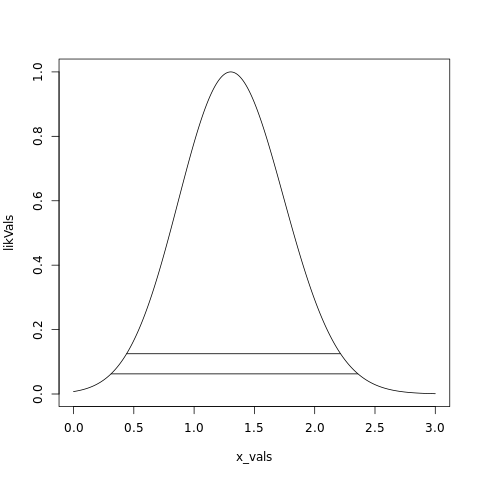
\includegraphics[scale=.5]{figs/non-central-tdis-mu-div-sigma-likelihood.png}
    \caption{Likelihood plot for the effect size $\frac{\mu}{\sigma}$ for the non-central \tdis. }
    \label{fig:likplot_nctdis}
\end{figure}

\underline{\textbf{Profile Likelihoods:}}

To obtain a likelihood for $\mu$ alone, the preferred method is called profiling. The profile for parameter $\mu_0$ is obtained by maximizing the joint likelihood for $\sigma$ with $\mu$ fixed at $\mu_0$, this process being repeated for many values of $\mu_0$.

Consider a joint likelihood with $\mu$ fixed at $\mu_0$ given by 

$$
\propto \prod_{i=1}^{n} \Bigg[(\sigma^2)^{-\frac{1}{2}} \exp\bigg(-\frac{(x_i-\mu_0)^2}{2\sigma^2}\bigg)\bigg].
$$

With $\mu_0$ fixed, the ML estimator for $\sigma^2$ is $\hat{\sigma} = \frac{1}{n} \sum_{i=1}^{n} (x_i-\mu_0)^2$\footnote{This result is similar in nature to the sample variance, but not exactly since $\mu_0$ is not the sample mean but rather some arbitrary, fixed, number.}. Plugging this into the likelihood returns 

$$
\bigg(\sum_{i=1}^{n} \frac{(x_i-\mu_0)^2}{n}\bigg)^{-\frac{n}{2}} e^{-\frac{n}{2}}.
$$

Therefore, up-to multiplicative constants, the profile likelihood is

$$
\bigg(\sum_{i=1}^{n} \frac{(x_i-\mu_0)^2}{n}\bigg)^{-\frac{n}{2}},
$$

which is clearly maximized at $\mu = \bar{\X}$, the same as the ML estimate for $\mu$ for the complete likelihood. This profile likelihood is presented at \ref{fig:prof_lik} using the sleep dataset with the following R code:

\begin{lstlisting}[language=R]
data(sleep)

g1 <- sleep$extra[1:10]
g2 <- sleep$extra[11:20]
l1 <- length(g1); l2 <- length(g2)

if (l1 == l2){
    diff <- g2 - g1
    n <- length(g1)
} else{
    print("Incompatible list dimensions")
} 

mean_diff <- mean(diff)

muvals <- seq(0, 3, length = 10^3)

prof_lik <- function(mu){
            (sum((diff-mu)^2)/sum((diff-mean_diff)^2))^(-n/2)
            }

likelihood_vals <- sapply(muvals, prof_lik)
plot(muvals, likelihood_vals,type='l')
\end{lstlisting}

\begin{figure}
    \centering
    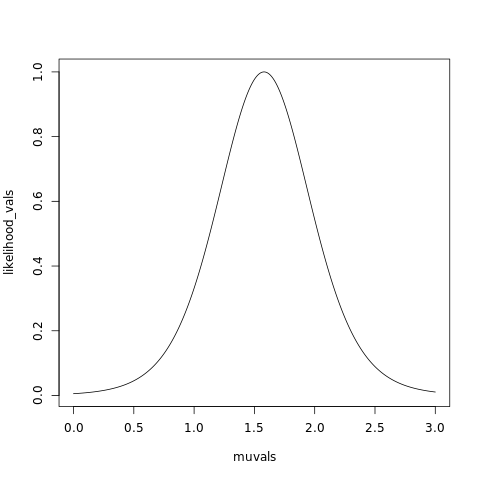
\includegraphics[scale=0.5]{figs/plotting profile likelihood for mu.png}
    \caption{Plot of the profile likelihood for $\mu$ of joint likelihood distribution for $n$ iid gaussian $\N(\mu,\sigma^2).$}
    \label{fig:prof_lik}
\end{figure}

\textnormal{ } \\

\paragraph{\textbf{{$t$-confidence intervals}}}

As motivation for developing confidence intervals using the \tdis, suppose that we desire to compare mean blood pressure between two group in a randomized trial, those who received the treatment versus those who received a placebo. We can't use a paired $t$-test (basically, taking differences of the data) since the groups are independent and may have different sample sizes. There are, however, different methods for comparing independent groups. \\

We're interested in constructing a $t$-interval for the variance, supposing the treated and control group have the same variance, 

\begin{itemize}
    \item Let ${\bf X}_1, \cdots, {\bf X}_{n_x}$ be iid $\N(\mu_x,\sigma^2)$, the first group's data,
    \item let ${\bf Y}_1, \cdots, {\bf Y}_{n_y}$ be iid $\N(\mu_y,\sigma^2)$,  the first group's data,
    \item let $\bar{\bf X}$, $\bar{\bf Y}$, ${\bf S}_x$ and ${\bf S}_y$ be the means and standard deviations respectively.
\end{itemize}

Using the fact that linear combinations of normal random variables are again normal random variables, we know that $\bar{\bf Y}-\bar{\bf X} \sim \N(\mu_Y-\mu_X, \sigma^2\bigg(\frac{1}{n_x}+\frac{1}{n_y}\bigg))$, then the pooled variance estimator

\begin{align*}
{\bf S}_p^2 &= \frac{(n_x-1){\bf S}_x^2+(n_y-1){\bf S}_y^2}{n_x+n_y-2} \\
&= \pi {\bf S}_x^2 + (1-\pi) {\bf S}_y^2 \textnormal{ where } \pi=\frac{n_x-1}{n_x+n_y-2} 
\end{align*}

is a good estimator for $\sigma^2$. It's a mixture of the group variances, placing greater weight on whichever has a larger sample size. Should the sample sizes be equal, the pooled variance estimate is the average of the group variances. As an estimator, it's unbiased since 

\begin{align*}
    \E({\bf S}_p^2) &= \frac{(n_x-1)\E({\bf S}_x^2)+(n_y-1)\E({\bf S}_y^2)}{n_x+n_y-2} \\
    &= \frac{(n_x-1)\sigma^2+(n_y-1)\sigma^2}{n_x+n_y-2}.
\end{align*}

Note that the pooled variance estimate is independent of $\bar{\bf Y}-\bar{\bf X}$ since ${\bf S}_x$ is independent of $\bar{\bf X}$ and ${\bf S}_y$ is independent of $\bar{\bf Y}$. The sum of two independent \chidis random variables is again another random variable with its degrees of freedom being the sum of the degrees of freedom of the summands. Therefore, remembering that ${\bf V} = (n-1) \frac{{\bf S}_{n}^2}{\sigma^2} \sim \chi^2_{n-1}$ then

\begin{align*}
    (n_x+n_y-2)\frac{{\bf S}_{p}^2}{\sigma^2} = (n_x-1) \frac{{\bf S}_{x}^2}{\sigma^2} + (n_y-1) \frac{{\bf S}_{y}^2}{\sigma^2} \\
    &\sim \chi^2_{n_x-1} + \chi^2_{n_y-1} \\
    &\sim \chi^2_{n_x+n_y-2}
\end{align*}

This is useful to create a pivot, since a $t$-confidence intervals are constructed by getting a standard normal out of the data and dividing it by its degrees of freedom and the squared root of a \chidis, in other words

$$
\frac{{\bf Z}}{\sqrt{\frac{{\bf V}}{n-1}}} =  (\bar{\X}_n - \mu) \frac{\sqrt{n}}{S_n} \sim t_{n-1}.
$$

Then the statistic 

$$
\frac{\frac{\bar{{\bf Y}}-\bar{{\bf X}} - (\mu_Y-\mu_X) }{\sigma\left(\frac{1}{n_X}+\frac{1}{n_Y}\right)}}{\sqrt{\frac{(n_X+n_Y-2){\bf S}_p^2}{n_X+n_Y-2\sigma^2}}} \sim \frac{\N(0,1)}{\sqrt{\frac{\chi^2_{n_x+n_y-2}}{{n_x+n_y-2}}}},
$$

which can be rewritten as 

$$
 \frac{\bar{{\bf Y}}-\bar{{\bf X}}- (\mu_Y-\mu_X)}{{\bf S}_p \left(\frac{1}{n_X}+\frac{1}{n_Y}\right)^{1/2}} \sim t_{n_x+n_y-2}
$$


a standard normal (since $\bar{Y}-\bar{X} \sim \mathcal{N}\left(\mu_{Y}-\mu_{X},\sigma^2 \left(\frac{1}{n_X}+\frac{1}{n_Y}\right)\right)$) divided by  the square root of an independent Chi-squared divided by its degrees of freedom. Thus, this statistic follows a Gosset's $t$ distribution with $n_X+n_Y-2$ degrees of freedom. This is a special case of an ANOVA test. \\

Therefore a $(1-\alpha)\times 100\%$-confidence interval for $\mu_Y-\mu_X$ can be written as follows

$$
\bar{Y}-\bar{X}\pm t_{n_{X}+n_{Y}-2,1-\frac{\alpha}{2}}S_p \sqrt{\frac{1}{n_X}+\frac{1}{n_Y}}.
$$

Notice that the previous random variable follows a non-central $t$-distribution with non-centrality parameter given by $ \frac{(\mu_Y-\mu_X)}{{\bf S}_p \left(\frac{1}{n_X}+\frac{1}{n_Y}\right)^{1/2}}$. Then we can use this statistic to create a likelihood for $\frac{\mu_Y-\mu_X}{\sigma}$, a standardized measure of the change in group means. \\

If we're unwilling to assume equal variances accross the two data groups, we can assert that 

$$
\bar{{\bf Y}}-\bar{{\bf X}} \sim \N\bigg(\mu_Y-\mu_X, \frac{\sigma^2_x}{n_x}+\frac{\sigma^2_y}{n_y}\bigg),
$$

since we can't factor out $\sigma^2$ out of the square root, then the statistic

$$
\bar{Y}-\bar{X}\pm t_{n_{X}+n_{Y}-2,1-\frac{\alpha}{2}}S_p \sqrt{\frac{1}{n_X}+\frac{1}{n_Y}},
$$

approximately follows a Gosset's \tdis with its degrees of freedom equal to 

$$
\frac{(\frac{{\bf S}_x^2}{n_x}+\frac{{\bf S}_y^2}{n_y})^2}{\bigg(\frac{{\bf S}_x^2}{n_x}\bigg)^2 \frac{1}{n_x-1}+\bigg(\frac{{\bf S}_y^2}{n_x}\bigg)^2 \frac{1}{n_y-1}}.
$$

The confidence interval can be readily computed using the appropriate $t$-quantile. 

\subsection{Week 4}

\clearpage

\section{Part 2}
\subsection{Week 1}

\subsubsection{Hypothesis testing}

Hypothesis testing is concerned with making decisions using data. We label a null hypothesis as $H_0$. The null hypothesis is assumed true and statistical evidence is required to rejected in favour of an alternative hypothesis. \\

For example, a respiratory disturbance index of more than 30 events/hour is considered evidence of severe sleep disorder breathing. Suppose that in a sample of 100 overweight subjects with other risk factors for sleep disordered breathing at a sleep clinic, the mean RDI was 32 events/hour with a standard deviation of 10 events/hour. We might want to test the hypothesis that 

\begin{itemize}
    \item $H_0 : \mu = 30$ 
    \item $H_a : \mu > 30$ 
\end{itemize}

where $\mu$ is the population mean RDI. The alternative hypothesis are typically of the form $<,> or \neq$. Note that there four possible outcome of our statistical decision process\\

\begin{center}
\begin{tabular}{ |p{1cm}||p{5cm}|p{5cm}|  }
 \hline
 \multicolumn{3}{|c|}{Statistical decision process} \\
 \hline
 Truth& $H_0$ & $H_a$\\
 \hline
 $H_0$  & Correctly accept null & Type I error\\
 $H_a$ &  Type II error & Correctly reject null\\
 \hline
\end{tabular}
\end{center}

\begin{itemize}
    \item The type I error rate is a false positive \textit{ie.} the mistaken rejection of a (true) null hypothesis. 
    \item The type II error rate is a false negative \textit{ie.} the mistaken acceptance of a (false) null hypothesis, we failed to reject a false $H_0$.
\end{itemize}

Let $\alpha$ denote the type I error rate, the probability of rejecting the null hypothesis when, in fact, then null hypothesis is correct. We'd like to minimise this kind of error. Considering our previous example, a reasonable strategy would reject the null hypothesis if $\Bar{X}$ was larger than some constant $C \in \mathds{R}_{+}$. Typically, $C$ is chosen so that the probability of a Type I error $\alpha$ is 0.05. \\

For example, the probability of a Type I error and according to the Central Limit Theorem we have  

\begin{align*}
        .05 &= \mathds{P}\bigg(\Bar{X}\geq C \bigg| \mu = 30 \bigg) \\
        &=\mathds{P}\bigg(\frac{\Bar{X}-30}{10/\sqrt{100}}\geq \frac{C-30}{10/\sqrt{100}} \bigg| \mu = 30 \bigg) \\
        &= \mathds{P}\bigg(Z\geq \frac{C-30}{10/\sqrt{100}}\bigg)
\end{align*}

Hence $\frac{C-30}{1}=1.645$ implying $C=31.645$. Now, since our mean is $32$ we reject the null hypothesis. We can plot a the 95th percentile of the standard normal distribution with the following R routine:

\clearpage

\begin{lstlisting}[language=R]
xval <-  seq(-3.2, 3.2, length=1000)
yval <- dnorm(xval)
plot(xval, yval, type="l", axes=TRUE, frame=FALSE, lwd=3, xlab="", ylab="")
x <- seq(qnorm(.95), 3.2, length=1000)
polygon(c(x,rev(x)), c(dnorm(x), rep(0, length(x))), col="salmon")
text(mean(x), mean(dnorm(x))+0.2, "5%", cex=2)
text(qnorm(.95), .01, "1.645",cex=2),
\end{lstlisting} 

which outputs plot \ref{fig: normal Z test}. 

\begin{figure}
    \centering
    \includegraphics[scale=0.4]{figs/95th percentile of a gaussian.png} 
    \caption{R-generated plot of the standard normal distribution $\mathcal{N}(0,1)$,  in the [-3.2, 3.2] range. The shaded polygon represents the 95th percentile (which is given by $x=1.645$) of a standard normal distribution. }
    \label{fig: normal Z test}
\end{figure}

In general, we don't convert $C$ back to its original scale. We would just reject it because the Z-score, how many standard error units the sample mean is above the hypothesised mean, is greater than $1.645$ \textit{ie. }

$$
\frac{32-30}{10/\sqrt{100}} = 2 > 1.645.
$$

Our mean is two standard error units away from the hypothesised mean. We can codify these rules for a normal Z test, assuming the data is gaussian or that the Central Limit Theorem is a good enough approximation to apply, as follows:

\begin{tcolorbox}[title=Rules for a normal Z-test]

Let $H_0 : \mu = \mu_0$ be the null hypothesis, then let 
\begin{itemize}
    \item $H_1: \mu < \mu_0$
    \item $H_2: \mu \neq \mu_0$
    \item $H_3: \mu > \mu_0$
\end{itemize}

where the test statistic $TS = \frac{\Bar{X}-\mu_0}{S/\sqrt{a}}$ (expressing the mean in standard error units), where $S/\sqrt{a}$ is the standard error. Thus, we reject the null hypothesis when 

\begin{itemize}
    \item $H_1: TS \leq -z_{1-\alpha}$ \textit{ie.} we reject $H_0$ in favour of $H_1$ if our sample mean is enough below $\mu_0$,
    \item $H_2: |TS| \geq  z_{1-\alpha/2}$ \textit{ie.} we reject in favour of $H_2$ if our sample mean is enough too different from $\mu_0$ (either too large or too small)\footnote{In this case, we look at the $(1-\alpha/2)\times 100\%$ error rate, we divide the probability of a type I error into half of it being accidentally rejected because of sample mean being too large and the other half of it being accidentally rejected because the sample mean is too small. }, 
    \item $H_3: TS \geq z_{1-\alpha}$ \textit{ie.} we reject in favour of $H_3$ if our sample mean is enough above $\mu_0$.
\end{itemize}
\end{tcolorbox}

The region of TS values for which the null hypothesis is rejected is the rejection region. In the case of $H_1$, the upper normal quantile and above is the rejection region, for $H_2$ it's the negative quantile and below or the upper quantile and above and finally, in the case of $H_3$, the normal quantile and below is the rejection region. We can graphically represent the second case, the case of a two-sided tail test, with the following R routine

\begin{lstlisting}[language=R]
xval <-  seq(-3.2, 3.2, length=1000)
yval <- dnorm(xval)

plot(xval, yval, type = "l", axes=TRUE, frame=FALSE, lwd = 3, xlab="", ylab= "")
x <- seq(qnorm(.975), 3.2, length = 100)
polygon(c(x, rev(x)), c(dnorm(x), rep(0,length(x))), col="salmon")
text(mean(x), mean(dnorm(x))+0.2, "2.5%", cex=2)
text(qnorm(.975), .01, "1.96",cex=2)

x <- seq(-3.2, qnorm(0.025), length=100)
polygon(c(x, rev(x)), c(dnorm(x), rep(0,length(x))), col="salmon")
text(mean(x), mean(dnorm(x))+0.2, "2.5%", cex=2)
text(qnorm(.025), .01, "1.96",cex=2)
text(0, dnorm(0)/5, "95%",cex=2)
\end{lstlisting}

\begin{figure}
    \centering
    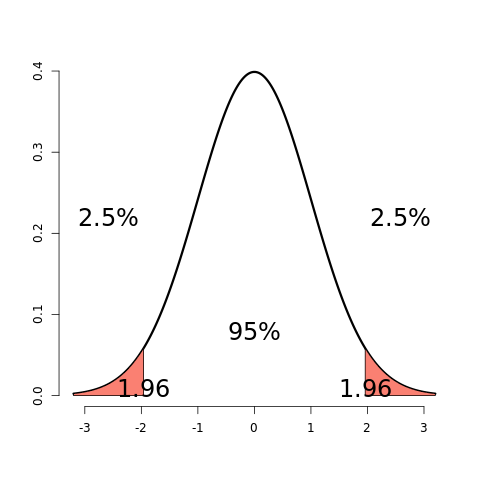
\includegraphics[scale = 0.4]{figs/two sided tail test.png}
    \caption{Two sided tail test presenting a standard normal $\mathcal{N}(0,1)$ distribution. We're going to reject $H_0$ if our test statistic is above $1.96$ -which has a 2.5\% chance under the null hypothesis- and we're going to reject $H_0$ if our test statistic is below $-1.96$ -which also has a 2.5\% chance under the null hypothesis-. Thus the union of those two events has a 5\% chance under the null hypothesis. }
    \label{fig:my_label}
\end{figure}

In hypothesis testing, we fix the $\alpha$ (type I error value) to be low. So if we reject the null hypothesis, either our model is wrong or there is a low probability that we made and error. We haven't fixed the probability of a type II error $\beta$, therefore we tend to say "fail to reject $H_0$" rather than accepting $H_0$. In general, less is known about the type II error. Statistical significance is not the same as scientific significance. 

\clearpage

\subsubsection{Two sided tests}

The Z-test requires the assumption of the Central Limit theorem and for $n$ to be large enough for the CLT to apply. If $n$ is mall, then a Gossett's $T$ test is performed exactly in the same way with the normal quantiles being replaced by the appropriate Student's $T$ quantiles and $n-1$ degrees of freedom. 

The probability of rejecting a false null hypothesis is called \textbf{power}. The statistical power of a dichotomic (binary) hypothesis test is the probability that the test correctly rejects the null hypothesis $H_0$ when a specific alternative hypothesis $H_1$ is true\footnote{Remember that the probability of rejecting a true null hypothesis is the type I error rate and is set to be small whilst the probability of failing to reject (this is the mistaken acceptance) a false null hypothesis is called a type II error rate. The power is $1-\beta$.}. A high value of power is good thing, we want to reject a false null hypothesis but it's not an easy to manipulate quantity in an experiment. One way to combat this issue is, prior to conducting the study, to do a power calculation of the sample size to obtain a certain level of power using guesses for the standard deviation and the hypothesised significant effect.

For example, suppose that $n=16$ (rather than 100) in our previous example. Instead of using a Z-test, we use a Student's $T$-test. Then 

$$
.05 = \mathds{P}\bigg(\frac{\Bar{X}-30}{s/\sqrt{16}} \geq t_{1-\alpha, 15} \bigg| \mu = 30\bigg)
$$

where $s/\sqrt{16}$ is the estimated standard error, where $t_{1-\alpha, 15}$ is t-quantile. Then our test statistic is now $\sqrt{16}\frac{32-30}{10} = .8$, while the critical value is $t_{1-\alpha, 15} = 1.75$. Thus, we fail to reject the null hypothesis. Remember that T has a heavier tail distribution than the normal distribution.

We are now interested in a two sided test. We are interested in studying if our hypothesised mean is significantly larger than $30$ or significantly smaller than $30$. That is, we want to test he alternative hypothesis $H_a: \mu \neq 30$. Then

$$
\alpha = \mathds{P}\bigg(\bigg|\frac{\Bar{X}-30}{s/\sqrt{16}}\bigg| > t_{1-\alpha/2, 15}\bigg| \mu = 30\bigg),
$$

that is: we'll reject $H_0$ is the test statistic (0.8) is either too large or two small with the critical value being calculated using $\alpha/2$. In our example, this critical value is $2.13$ so we fail to reject it\footnote{We note that, if the data are iid Gaussians, then $\frac{X-\mu}{s/\sqrt{n}} \sim t_{n-1}$} The previous calculation can be understood with the following R routine 

\begin{lstlisting}[language=R]
xval <-  seq(-4, 4, length=1000)
yval <- dt(xval, 15)
plot(xval, yval, type = "l", axes=TRUE, frame=FALSE, lwd = 3, xlab="", ylab= "")
x <- seq(qt(.975, 15), 4, length=100)
polygon(c(x, rev(x)), c(dt(x,15), rep(0,length(x))), col="salmon")
text(mean(x), mean(dt(xval, 16-1))+0.2, "2.5%", cex=2)
text(qt(.975,15), .01, "2.13",cex=2)
x <- seq(-3.2, qt(.025,16), length=100)
polygon(c(x, rev(x)), c(dt(x,15), rep(0,length(x))), col="salmon")
text(mean(x), mean(dt(xval, 16-1))+0.2, "2.5%", cex=2)
text(qt(.025,15), .01, "2.13",cex=2)
text(0, dt(0,15)/5, "95%", cex=2)
\end{lstlisting}

which outputs figure \ref{fig: two sided Student's T test}. \\

\clearpage

\begin{figure}
    \centering
    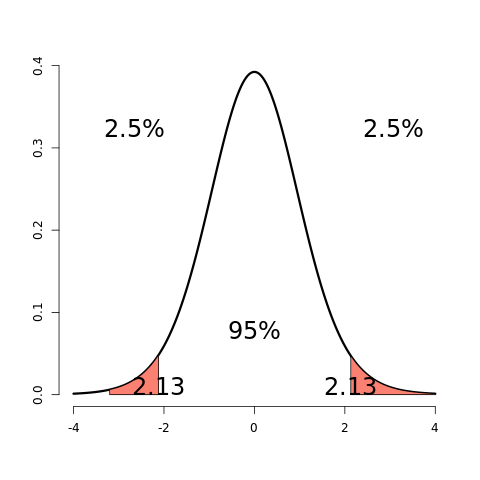
\includegraphics[scale=0.4]{figs/two sided T test.png}
    \caption{We calculate our normalised test statistic $\frac{\Bar{X}-\mu}{s/\sqrt{n}}$ and the probability that the absolute value of said statistic is bigger than $2.13$ \textit{ie.} the probability that the statistic is too large positive than $2.13$ is 2.5\% or too small negative than $-2.13$ is 2.5\%. In our case, the probability that the test statistic lies in the rejection region is 5\%. For the $T$ distributionwith 15 degrees of freedom, the 97.5th quantile is 2.13 and the 2.5th quantile is $-2.13$. }
    \label{fig: two sided Student's T test}
\end{figure}

\subsubsection{Confidence intervals and P values}

Consider testing $H_0 : \mu = \mu_0$ versus $H_a : \mu \neq \mu_0$. Take the set of all possible values for which we fail to reject $H_0$, this set is a $(1-\alpha)\times 10\%$ confidence interval for $\mu$, these are the value for $\mu$ that are supportable as null hypotheses (those are reasonable numbers for $\mu$). This rule works both ways, if a $(1-\alpha)\times 10\%$ contains $\mu_0$, then we fail to reject $H_0$.

Consider that we don't reject $H_0$ if our test statistic behaves as follows:

$$
\bigg|\frac{\Bar{X}-\mu}{s/\sqrt{n}}\bigg| \leq t_{1-\alpha/2, n-1},
$$

which implies 

$$
|\Bar{X}-\mu| \leq t_{1-\alpha/2, n-1} s/\sqrt{n}
$$

which, in turn, implies that 

$$
\bar{X} - t_{1-\alpha/2, n-1} \frac{s}{\sqrt{n}} < \mu_0 < \bar{X} + t_{1-\alpha/2, n-1} \frac{s}{\sqrt{n}}.
$$

This states that if $\mu_0$ lies inside the confidence interval, the we've failed to reject $H_0$ and this argument is reversible. This establishes a duality between confidence intervals and two-sided hypotheses tests. If we create a 95\% confidence interval, it conveys more information than the result of a hypothesis test because we can do the hypothesis test and gives a sense of what values for $\mu_0$ are well supported, helping to reduce the gap between statistical significance and scientific significance. 

In our previous example, we rejected the one-sided test when $\alpha = .05$, would we reject it if $.01$ or $.001$?

The smallest value for $\alpha$ that you still reject the null hypothesis is called the \textbf{attained significance level}. This equivalent, but philosophically different, from the \textbf{P-value}.
The P-value (same number but different concept) is the probability, under the null hypothesis, of obtaining evidence as extreme or more extreme than would be observed by chance alone, where chance is governed by the null distribution. If the P-value is small, then either $H_0$ is true and we have observed a rare event, given that the null hypothesis is true, or $H_0$ is false. It quantifies whether or not getting a test statistic as or more extreme than you observed was rare under the null hypothesis. If it's rare, then that casts some doubt on the veracity of the null hypothesis. \\ 

In our example, the $T$ statistic was $0.8$. What's the probability of getting a $T$ statistic as large as $0.8$? This can be computed with the following R code 

\begin{lstlisting}[language=R]
pt(0.8, 15, lower.tail = FALSE) 

In [1]:  0.218099
\end{lstlisting}

where \texttt{pt} stands for $T$ probability, \texttt{lower.tail = FALSE} indicates we want a value above $0.8$, not lower. This works out to be $P = 22\% > \alpha = 5\%$, which is entirely reasonable because we failed to reject the null hypothesis. 

\begin{itemize}
    \item If the P-value is larger than $\alpha$, we fail to reject $H_0$. 
    \item If the P-value is smaller than $\alpha$, we reject $H_0$
\end{itemize}

This can be understood via the following R routine 

\begin{lstlisting}[language=R]
pt(0.8, 15, lower.tail=FALSE)
xval <-  seq(-4, 4, length=1000)
yval <- dt(xval, 15)
plot(xval, yval, type = "l", axes=TRUE, frame=FALSE, lwd = 3, xlab="", ylab= "")
x <-  seq(.8, 4, length=100)
polygon(c(x, rev(x)), c(dt(x,15), rep(0,length(x))), col="salmon")
text(mean(x), mean(dt(xval, 16-1))+0.2, "22%", cex=2)
text(.8, .01, "0.8",cex=2)
\end{lstlisting}

which outputs figure \ref{fig: P-value T statistic}.

\begin{figure}
    \centering
    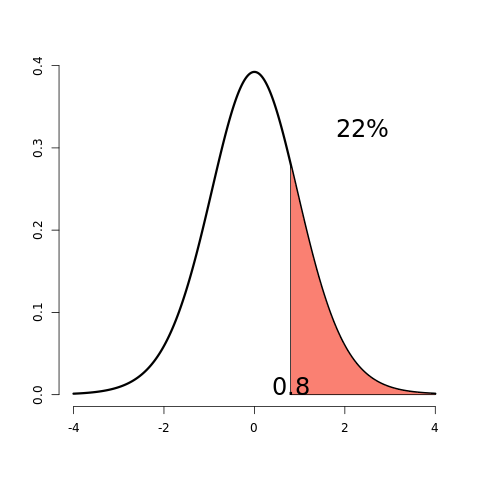
\includegraphics[scale = .4]{figs/P-value T statistic.png}
    \caption{Our statistic $\frac{\bar{X}-\mu}{s/\sqrt{n}}$ turned out to be .8. The probability of being .8 or larger for a Student's $T$ distribution with 15 degrees of freedom is $22\%$. Since this number is larger than $\alpha = 5\%$, we would fail to reject $H_0$. }
    \label{fig: P-value T statistic}
\end{figure}

By reporting a P-value, the reader can perform a hypothesis test at whatever $\alpha$ level he or she chooses. Again, is the P-value is less than $\alpha$, we reject the null hypothesis.

For two sided hypothesis test, double the smaller of the two one sided hypothesis test P-values. \\ 

Criticisms of the P value:

\begin{itemize}
    \item P values only consider significance, unlike confidence intervals making it harder to distinguish practical significance from statistical significance.
    \item Absolute measures of the rareness of an event are not good measures of the evidence for or against a hypothesis.
\end{itemize}

\clearpage

\subsubsection{Power}

Power is the probability of rejecting the null hypothesis when it's false. And, as the name suggests, it's a desirable quality, the more power, the more reliable the test is. A type II error is failing to reject the null hypothesis when it's false. Thus, by their definitions, power + type II error rate ($\beta$) sum to one. Thus we define $\textnormal{Power} = 1- \beta$.

Consider the example involving RDI. The null hypothesis is $H_0 : \mu = 30$ versus $H_a : \mu > 30$. Then power is calculated under the alternative hypothesis, as follows  

$$
\mathds{P}\bigg(\frac{\bar{X}-30}{s/\sqrt{n}} > t_{1-\alpha, n-1} \bigg | \mu = \mu_a\bigg).
$$

The power of the test is the probability that the $T$ statistic lies in the rejection region. If this normalised mean was greater than the $t_{1-\alpha, n-1}$ quantile, then we reject the null hypothesis. Note that this quantity is calculated not under the assumption of the null hypothesis but rather calculated under the assumption of the alternative hypothesis. Note that this function depends on the specific value of $\mu_a$ and we notice that, as $\mu \rightarrow 30$, power approaches $\alpha$. 

\subsubsection{Calculating Power}

Assume that $n$ is large, thus the central limit theorem holds - allowing us to use standard normal calculations rather than $T$ calculations-, and we know $\sigma$, then

\begin{align*}
        1- \beta &= \mathds{P}\bigg(\frac{\bar{X}-30}{\sigma/\sqrt{n}} > z_{1-\alpha}\bigg|\mu = \mu_a\bigg) \\
    &= \mathds{P}\bigg(\frac{\bar{X}-\mu_a+\mu_a-30}{\sigma/\sqrt{n}}\bigg| \mu = \mu_a\bigg) \\
    &= \mathds{P}\bigg(\frac{\bar{X}-\mu_a}{\sigma/\sqrt{n}}> z_{1-\alpha}-\frac{\mu_a-30}{\sigma/\sqrt{n}}\bigg|\mu = \mu_a\bigg) \\
    &= \mathds{P}\bigg(Z > z_{1-\alpha} -\frac{\mu_a-30}{\sigma/\sqrt{n}} \bigg|\mu = \mu_a\bigg)
\end{align*}

In the first line we have our test statistic $\frac{\bar{X}-30}{\sigma/\sqrt{n}}$, which under the null hypothesis $H_0 : \mu = 30$ is a $Z$-statistic, but we are going to calculate it under the alternative hypothesis. Hence, our rejection region will be for the normalised mean values larger than a standard normal quantile. Then $1-\beta$ is the probability we reject a false null hypothesis, it's the probability that the statistic is larger than the quantile (the cutoff value), given that $\mu$ is in fact $\mu_a$. 
Since we are considering the alternative hypothesis and not the null hypothesis, this quantity -$\frac{\bar{X}-30}{\sigma/\sqrt{n}}$- is no longer a $Z$-statistic but it's normal should the data be iid Gaussian. 

In line 2, we convert it into a $Z$-statistic by adding and subtracting $\mu_a$. In line 3 we take the correctly normalised mean $\frac{\bar{X}-\mu_a}{\sigma/\sqrt{n}} \sim \mathcal{N}(0, 1)$ which is in fact a $Z$-statistic (under the alternative hypothesis), and we calculate the probability that said quantity is larger than $z_{1-\alpha}-\frac{\mu_a-30}{\sigma/\sqrt{n}}$. 
In line 4, we calculate the probability of $Z$ being larger than $z_{1-\alpha}-\frac{\mu_a-30}{\sigma/\sqrt{n}}$, which can be easily computed provided $\sigma$ is known and a $\mu_a$ value has been selected. \\

\begin{tcolorbox}[title=Example]

\textbf{Statement}: Suppose we wanted to detect an increase in mean RDI of at least 2 events/hours above 30. Assume normality and setting a type I error rate of 5\% and that the sample in question will have a standard deviation of 4, what would be the power if we took a sample size of 16?

Now, $Z_{1-\alpha} = 1.645$ and $\frac{\mu_a-30}{\sigma/\sqrt{n}} = 2$. Then $\mathds{P}(Z > 1.645 - 2)  = \mathds{P}(Z > -0.355) = 64\%$

So under these settings, the probability of detecting an alternative of two events above the hypothesised value per hour is 64\%. Note that this is only a bound for all values above 32\%, the power gets larger as the alternative goes away from 30 events per hour.

\end{tcolorbox}

\begin{tcolorbox}[title=Example of a Sample Size Calculation]
Suppose we have a power we want to achieve for a particular value of the alternative, what sample size would we need to achieve it? What $n$ would be required to get a power of 80\%?

We want to compute the following expression and solve for $n$

$$
0.8 = \mathds{P}\bigg(Z > z_{1-\alpha} -\frac{\mu_a-30}{\sigma/\sqrt{n}} \bigg|\mu = \mu_a\bigg)
$$

where the $Z$-statistic is in fact normalised under the alternative hypothesis. We set $z_{1-\alpha} -\frac{\mu_a-30}{\sigma/\sqrt{n}}  = z_{0.20}$, the 20th quantile of the standard normal distribution and solve for $n$. This guarantees a 80\% or higher power, so $\mu_a$ is typically the smallest effect which can be reasonably detected. The calculation for $H_a: \mu < \mu_0$ is similar. 
\end{tcolorbox}

In general, for $H_a : \mu \neq \mu_0$ we calculate the one sided power using $\alpha/2$ (this is only approximately right since it excludes the probability of getting a large TS in the opposite direction of the truth).

In conclusion

\begin{itemize}
    \item Power goes up as $\alpha$ gets larger, \item Power of a one sided test is greater than the power of the associated two sided test,
    \item Power goes up as $\mu_1$ gets further away from $\mu_0$ and power goes up as $n$ goes up.
\end{itemize}

Regarding the first item, if we're requiring less evidence to reject the null hypothesis, we're bound to detect more alternative hypotheses. \\


\subsubsection{T Tests and Monte Carlo}

\paragraph{\textbf{Power for the T test}}: Consider calculating power for a Gossett's $T$ test for our example. The power is 
\begin{align*}
\mathds{P}\bigg(\frac{\bar{X}-30}{S/\sqrt{n}}>t_{1-\alpha, n-1}\bigg|\mu = \mu_a\bigg)  &= \mathds{P}\bigg(\sqrt{n}(\bar{X}-30)>t_{1-\alpha, n-1}S\bigg| \mu = \mu_a \bigg) \\
&= \mathds{P}\bigg(\frac{\sqrt{n}(\bar{X}-30)}{{\sigma}}>t_{1-\alpha, n-1}\frac{S}{\sigma}\bigg| \mu = \mu_a \bigg) \\
&= \mathds{P}\bigg(\frac{\sqrt{n}(\bar{X}-\mu_{a})}{{\sigma}}+\frac{\sqrt{n}(\mu_{a}-30)}{{\sigma}}>\frac{t_{1-\alpha, n-1}}{\sqrt{n-1}}\times \sqrt{\frac{(n-1)S^2}{\sigma^2}}\bigg| \mu = \mu_a \bigg) \\
&= \mathds{P}\bigg(Z+\frac{\sqrt{n}(\mu_{a}-30)}{{\sigma}}>\frac{t_{1-\alpha, n-1}}{\sqrt{n-1}} \sqrt{\chi^2_{n-1}}\bigg| \mu = \mu_a \bigg),
\end{align*}

where $Z \sim \mathcal{N}(0,1)$ is the independent standard normal and where $\chi^2_{n-1}$ is the chi-squared random variable with $n-1$ degrees of freedom. In regards to the first expression, the power is the probability that our test statistic lies in the rejection region and it's performed under the alternative hypothesis and, in regards to the second-to-last expression, if the data are iid Gaussian $\frac{(n-1)S^2}{\sigma^2} \sim \chi^2_{n-1}$ and can be computed with the Monte-Carlo method, by simulating pairs of $Z$ random variables and $\chi^2$ random variables and evaluating this inequality for every pair. Note that, in general, $\mu_a$ per sé needs not to be specified, what we need to know is how different is $\mu_a$ from $\mu_0$ in standard deviation units. This quantity, $\frac{\mu_a-\mu_0}{\sigma}$, is called an effect size is a unit free quantity. For example, a Monte Carlo simulation can be performed to calculate the last expression for the RDI example with the following R code

\begin{lstlisting}[language=R]
no_sim <- 100000 # number of simulation to perform 
n_dof <- 16 # number of degrees of freedom
sigma <- 4 # variance 
mu0 <- 30 # RDI mean under the null hypothesis
mua <- 32 # RDI mean under the alternative hypothesis
z <- rnorm(no_sim) # rnorm is the R function that simulates random variables having a specified normal distribution
chisq <- rchisq(no_sim, df = n_dof - 1) # chi squared distribution
t_qt <- qt(.95, n_dof-1) # 95th quantile for the Gossett's T distribution
mean(z + sqrt(n_dof)*(mua-mu0)/sigma > 
    t_qt/sqrt(n_dof-1)*sqrt(chisq))

In[1]: [1] 0.60517
In[2]: function (x, ...) 
In[3]: UseMethod("mean")
In[4]: <bytecode: 0x56366e096b50>
In[5]: <environment: namespace:base>
\end{lstlisting}

In the previous code snippet, we have a 100000 pairs of normal and chi squared random variables, generated with the \texttt{rnorm} and \texttt{rchisq} R-functions. The \texttt{mean(...)} function returns a vector of ones every time the LHS is bigger than the RHS and zeros every time the LHS is smaller than the RHS and computes the mean of said vector entries. The accuracy of this computation is upto $\mathcal{O}\bigg(\frac{1}{n^2}\bigg)$. \\

\subsubsection{Two Sample Tests - Matched Data I}

When comparing two groups, first and foremost we want to determine whether observations are paired or not\footnote{For example, consider a medical trial of some medication. In one case we randomize that treatment to one group of test subjects and randomize a placebo to the other group of test subjects. This is not paired as the groups are distinct. An instance where the data are paired is, for example, administering the medication and the placebo in some random order for every test subject. Now the data is paired since some test subjects received both the treatment and the control.}. When dealing with a single set of paired data, one strategy is to take the difference between the paired observation and do a single one-sample $t$ test of $H_0 : \mu_d = 0$ versus $H_0 : \mu_d \neq 0$ (or one of the other two alternatives). The desired test statistic

$$
\frac{\bar{X}_d - \mu_{d0}}{S_d/\sqrt{n}}
$$

where $\mu_{d0}$ is the value under the null hypothesis (typically 0), where $n$ is the number of pairs of observations (and not the total number of observations themselves). This is called the \textbf{ordinary paired two-group t-test}. \\

\subsubsection{Two Sample Tests - Matched Data II}

Let's consider an example of a paired $T$-test.

\begin{tcolorbox}[title=Example]
Consider Exam 1 and Exam 2 grades from a previous class. Is there any evidence that the second exam was easier or harder than the first? \\

Clearly, the data are paired since it's the same students measured twice. This question can be answered by examining if the mean of exam one is different from the mean of exam two. 
\end{tcolorbox}

In general, giver our data, we can compute this with the following R code 

\begin{lstlisting}[language=R]
diff <- test2 - test1  #pair difference
n <- sum(!is.na(diff)) #number of subjects: 49
mean(diff) #mean of the pair difference: 2.88
sd(diff) #standard deviation of the pair difference: 7.61
testStat <- sqrt(n) * (mean(diff) - 0)/sd(diff) #test Statistic: 2.65

#we get the p-value by multiplying the probability of getting a test statistic 
# as large or larger than 2.65 for a Gossett's T distribution with n-1 dof by two, since it's a two sided test
2 * pt(abs(testStat), n-1, lower.tail = FALSE) # Since we're working with 48 dof, there's little diference from calculating a pnorm or a pt

------

## or using the R function
t.test(diff)
\end{lstlisting}

In our case we get that there appears to be a difference between the means of exam 1 and exam 2. \footnote{Graphically this can be represented with a so called "Mean difference plot", first presented by Tukey and by J. Martin Bland \& Douglas G. Altman.}. \\

\subsubsection{Two Sample Tests - Regression to the Mean}

Francis Galton was the first to recognise that for matched data, high initial observations tended to be associated with lower second observations and low initial observations observations tended to be associated with higher second observations. For example, sons of very tall fathers tend to be a little shorter and fathers of very tall sons tend to be shorter. Another example would be that second exams for those who scored very high on a first exam tend to be a little lower. 

In order to explain this phenomena, consider plot \ref{fig: Matched data plot}. Imagine if the tests were completely random and the students were iid draws from said distribution, so the higher observations of the exam were random observations. So the probability of a second observation being that high is quite low, since it's more likely to be in the center of the distribution. Conversely, a very low test (something that had a very low probability of occurring given that it's already low), the probability of a second test being that low is small. And so if the pairs of observations are exactly noise, then you'll have a lot of regression in the mean. This is one extreme of complete variation and, for a given student, there's no trend between exam 1' score and exam 2' score.

Consider the other extreme, let's imagine that the test was a perfect adjudicator of student's abilities, that it is a perfectly calibrated instrument and that there is no noise. Then the student should ideally get exactly the same score on both exams. At which point, there'd be no variation around an identity line of Exam 2 v. Exam 1. This is an extreme of no variation where there is a 100\% correlation. Every other practical case lies somewhere in between those two extremes. 
\begin{figure}
    \centering
    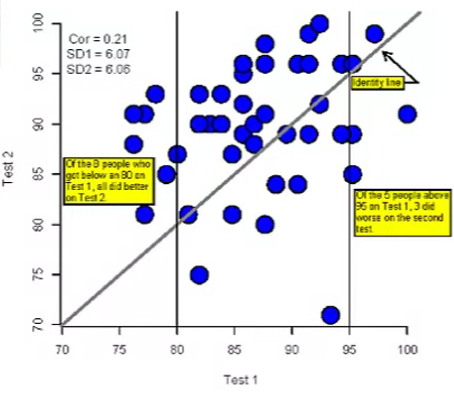
\includegraphics[scale = 0.4]{figs/Matched data plot.png}
    \caption{A matched data plot for the Exam 1 results v. Exam 2 results.}
    \label{fig: Matched data plot}
\end{figure}<

For example, of the eight people who got below 80 en the test, all did better on Test 2 and of the five people who got above a 95 test, three did worse on the second test. 

To investigate more, we normalise both scales (so that their empirical means are both 0 and their empirical standard deviations are 1). When asking questions about the paired data, we're asking questions about shifts in the means, information which we've gotten rid off. If there was no regression to the mean, the data would scatter about an identity line. The best fitting line goes through the average and has slope 

$$
\textnormal{Cor}(Test1, Test2) \frac{SD(Test2)}{SD(Test1)}
$$

and passes through the point 

$$
(\textnormal{mean}(Test1), \textnormal{mean}(Test2))
$$

Since we normalised the data, the best fitting line passes through (0,0) and has a slope of $\textnormal{Cor}(Test1, Test2) < 1$, since renormalizations don't affect the correlation. This will be shrunk toward a horizontal line, telling us our expected normalised test score for Test 2 is $\textnormal{Cor}(Test1, Test2)$ times the normalised Test 1 score. This line appropriately adjusts for regression to the mean for Test 2 conditioning on Test 1. We could similarly do the same for Test 1 conditioning on Test 2(in this case the best fitting line will have slope  
$\textnormal{Cor}(Test1, Test2)^{-1}$ if we plot with Test 1 on the Test 1 on the horizontal axis). The latter line will be shrunk toward a vertical line, the identity line will fall between the two. This can be better understood in plot \ref{fig: NTest2 v. NTest1}. In said plot we have the normalised Test 2 in the $y$-axis, the normalised Test 1 in the $x$-axis and the slope of the best regression line of Test 1 on Test 2 is the correlation between the two (0.21). In the middle we plot the identity line whilst the best regression line of Test 2 on Test 1 the slope is the inverse of the previous slope $1/0.2$. Note that all three lines pass through the (0,0).

\begin{figure}
    \centering
    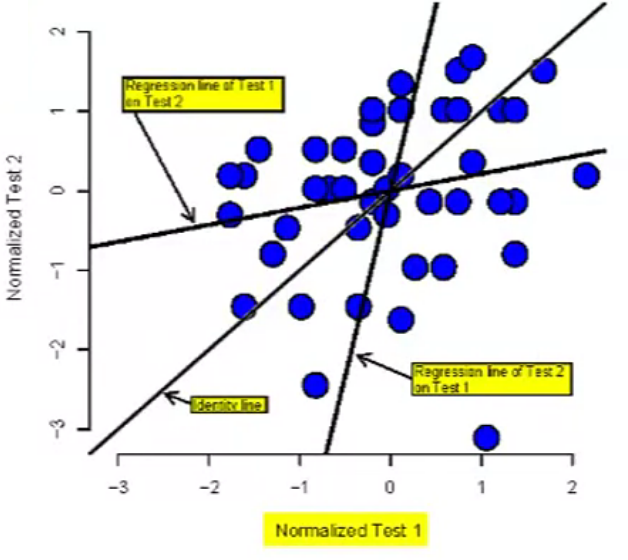
\includegraphics[scale=0.4]{figs/Normalised Test 2 v. Normalised Test 1 (adjusted).png}
    \caption{Normalised Test 2 scores v. Normalised Test 1 scores and the best fitting lines.  In this plot we have the normalised Test 2 in the $y$-axis, the normalised Test 1 in the $x$-axis and the slope of the best regression line of Test 1 on Test 2 is the correlation between the two (0.21). In the middle we plot the identity line whilst the best regression line of Test 2 on Test 1 the slope is the inverse of the previous slope $1/0.2$. Note that all three lines pass through the (0,0).}
    \label{fig: NTest2 v. NTest1}
\end{figure}

The line to be used when predicting test 2 scores from test 1 scores is a very flat (suggesting there's little correlation between the two tests, and this amount of noise also suggests there's a fair amount of regression to the mean) line whilst the line used to predict test 1 scores from test 2 scores is a very vertical line (because our correlation was quite low, suggesting a high amount of noise). Should the points collapse around an identity line, this suggests there's very little regression. 

In conclusion:

\begin{itemize}
    \item An ideal examiner would have little difference between the identity line and the fitted regression line.
    \item The more unrelated the two exam scores are the more pronounced the regression to the mean is.
\end{itemize} 

\clearpage

\subsubsection{Two Sample Tests - Two Independent Groups}

The extension to two independent groups is straightforward. Let $H_0 : \mu_1 = \mu_2$ versus $H_a: \mu_1 \neq \mu_2$ (or one of the other two alternatives). Assuming a common error variance we have that the following statistic

$$
\frac{\bar{X}-\bar{Y}}{S_p \sqrt{\frac{1}{n_X}+\frac{1}{n_Y}}} \sim t_{n_X+n_Y-2},
$$

under the null hypothesis $\bar{X}-\bar{Y}$ has a hypothesised mean of $0$ and if the data are iid Gaussian. In the limit of a large sample size, the previous statistic follows a normal distribution. If the assumption of a common error variance is questionable then 

$$
\frac{\bar{X}-\bar{Y}}{S_p \sqrt{\frac{1}{n_X}+\frac{1}{n_Y}}} \sim \mathcal{N}(0,1) \textnormal{ if } n_x, n_y \rightarrow \infty.
$$

where $S_p$ is the pooled variance. Furthermore, this statistic follows an approximate (only approximately, since the variances are not the same) Student's $T$ distribution if $X_i \sim \mathcal{N}(\mu_1,\sigma^2_1)$ and $Y_i \sim \mathcal{N}(\mu_2,\sigma^2_2)$. The approximate degrees of freedom are 

$$
\frac{(S_x^2/n_x+S_y^2/n_y)^2}{(S_x^2/n_x)^2/(n_x-1)+(S_y^2/n_y)^2/(n_y-1)}
$$

where $S_x$ and $S_y$ are the variances within group 1 and group 2 respectively. 

Note that the connection between hypothesis testing and confidence intervals still holds: for example, if zero is in our independent group $T$ interval, we will fail to reject the independent group $T$ test for equal means and viceversa, if we construct a confidence interval by finding all of the hypothesised values for differences of means for which we fail to reject the null hypothesis we wind up with the appropriate $t$ confidence interval. 

If we want to test equality of means, in general it's incorrect constructing separate confidence intervals, one CI for group I and another CI for group II, and seeing if those CIs overlap. This procedure only works if the CIs don't overlap and we reject, this is an accurate statement. But the confidence intervals can overlap and the correctly constructed test statistic would still reject, seemingly leading to a contradiction.  This procedure has lower power than the correctly implemented test.

\begin{tcolorbox}[title=Exam]

Suppose that instead of having repeated data on two consecutive exams, students were randomised to two teaching modules and took the same exam. We treat the data as independent group data. We might obtain data like the following 

Group || N || Mean Exam || SD Exam \\
Module 1 || 50 || 86.9 || 6.07 \\
Module 2 || 50 || 89.8 || 6.06 \\

The pooled standard deviation is 6.065 and the test statistic is 

$$
\frac{89.8-86.9}{6.065\sqrt{\frac{1}{50}+\frac{1}{50}}}
$$
\end{tcolorbox}

Suppose you have equal numbers of observations for two groups, $X$ and $Y$. If the data are truly matched, then the standard error of the difference is estimating 

$$
\sqrt{\frac{\sigma_x^2}{n}+\frac{\sigma_y^2}{n}-2\frac{\textnormal{Cov}(X,Y)}{n}}.
$$

If we ignore the matching by setting $\textnormal{Cov}(X,Y) = 0$, the standard error of the difference is estimating is estimating

$$
\sqrt{\frac{\sigma_x^2}{n}+\frac{\sigma_y^2}{n}}.
$$

Since, generally, matched data is positively correlated, by ignoring the matching, we are unnecessarily augmenting the standard error. 

\clearpage

\subsection{Week 2}

The score statistic is a specific two sample binomial test that will serve as motivation for creating a confidence interval

\subsubsection{Two sample Binomial Tests - Score Statistic}

Consider the following example

\begin{tcolorbox}[title=Example]

Consider a randomized trial where 40 subjects were randomized (20 each) to two drugs with the same active ingredient but different expedients. Consider counting the number of subjects with side effects for each drug. The gathered data is\\ 
    || Side Effects || None || Total \\
Drug A || 11 || 9 || 20 \\
Drug B || 16 || 15 || 20 \\
Total || 16 || 14 || 40 \\
\end{tcolorbox}

At first sight, there appears to be a higher propensity for side effects from Drug A than from Drug B. We'd like to do a test of whether or not the propensity of side effects is the same within the two drugs. 

Let's start with score tests. Consider testing the null hypothesis $H_0 : p = p_0$ for a binomial proportion. The \textbf{score test statistic} is constructed in the same way as a $Z$-test. Consider a single binomial proportion, only looking at drug A and considering if drug A has a specific population proportion of side effects

$$
\frac{\hat{p}-p_0}{\sqrt{p_0(1-p_0)/n}} \underset{n \rightarrow \infty}{\sim} \mathcal{N}(0,1).
$$

Note that $\sqrt{p_0(1-p_0)/n}$ is the standard error of the binomial distribution and we're using the null hypothesis\footnote{Should we use $\hat{p}$, we'd be constructing the estimated standard error, akin to the calculations of a confidence interval.}. This test performs better than the Wald test

$$
\frac{\hat{p}-p_0}{\sqrt{\hat{p}(1-\hat{p})/n}}.
$$

Both of the previous statistics are compared to the quantiles of the standard normal distribution, the upper $\frac{\alpha}{2}$th quantile for a two-sided test or the upper $\alpha$th quantile for an upper single-sided test where the alternative is $H_a : p > p_0$ and the $\alpha$th quantile for an upper single-sided test where the alternative is $H_a : p < p_0$. 

Inverting the Wald test yields the Wald interval, namely those values of $p_0$ for which we'd fail to reject the null hypothesis:

$$
\hat{p} \pm z_{1-\frac{\alpha}{2}}\sqrt{\frac{\hat{p}(1-\hat{p})}{n}}.
$$

Inverting the Score test yields the Score interval

\begin{equation*}
\hat{p}\bigg(\frac{n}{n+z^2_{1-\frac{\alpha}{2}}}\bigg) + \frac{1}{2}\bigg(\frac{z^2_{1-\frac{\alpha}{2}}}{n+z^2_{1-\frac{\alpha}{2}}}\bigg) \\
\pm z_{1-\frac{\alpha}{2}} \sqrt{\frac{1}{n+z^2_{1-\frac{\alpha}{2}}} \bigg[\hat{p}(1-\hat{p})\frac{n}{n+z^2_{1-\frac{\alpha}{2}{2}}}+\frac{1}{4}\frac{z^2_{1-\frac{\alpha}{2}}}{n+z^2_{1-\frac{\alpha}{2}}}\bigg] }
\end{equation*}

Note that $\frac{n}{n+z^2_{1-\frac{\alpha}{2}}}$ and $\frac{z^2_{1-\frac{\alpha}{2}}}{n+z^2_{1-\frac{\alpha}{2}}}$ add up to one, it's a point in the two-dimensional simplex. If $n \rightarrow \infty$ the first term dominates and $\hat{p}$ dominates, conversely if $n$ is small the second term dominates. 
Plugging $z_{1-\frac{\alpha}{2}} = 2$ yields the Agresti-Coull interval. As $n \rightarrow \infty$ this interval gets progressively similar to the Wald interval. This test takes $\hat{p}$ and shrinks it down to $\frac{1}{2}$ which is desired since for $p > \frac{1}{2}$, the binomial distribution gets progressively asymmetric. 

\begin{tcolorbox}[title=Example continued]

In our previous example consider testing whether or not Drug A's percentage of subjects with side effects is greater than 10\%. Then we'd like to test $H_0 : p_A = .1$ versus $H_a: p_A > .1$. Let $\hat{p} = 11/20 = .55$. Then our test statistic is 

$$
\frac{.55 - .1}{\sqrt{.1 \times .9/20}} = 6.7
$$

If we are performing a two-sided  95th $Z$-test, the quantile of interest is $1.645$ and if we're performing a one sided 95th $Z$-test the quantie of interest is $1.96$. In any case, $6.7 > z_{\textnormal{95th}}$, so we reject Our P-value, the probability of getting a $z$ bigger than $6.7$ is nearly around 0 (we're about six standard deviations from zero for a standard normal carries a very low probability since three standard deviations already covers the majority of the distribution).  For a two-sided test, we'd double this P-value.
\end{tcolorbox}

We're postulating the number of side effects out of 20 is a binomial trial. Implicit in this idea is the postulate of iid data, every person is an independent and identically distribution, drawn from a population. We use these ideas to construct a super population that has a prevalence of side effects of $p_A$. So our iid model is giving us an idea of a population proportion and we're testing relative to that proportion. 

\subsubsection{Two sample Binomial Tests - Exact Tests}

The previous method relies on the central limit theorem and having a large-enough sample size. It's possible to perform and exact binomial test. Consider calculating an exact P-value. What's the probability, under the null hypothesis, of getting evidence as extreme or more extreme than the one we obtained (ie. the probability of getting more than 11 people with side effects)?

$$
P(X_A\geq 11) = \sum_{x=11}^{20} {{20}\choose{x}} (.1)^x (.9)^{20-x} \approx 0.
$$

This calculation, the probability of getting more than 11 people with side effects out of 20, is done under the null hypothesis $H_0 : p_0 = 10\%$. This is the probability of getting evidence as or more extreme - in favour of the alternative - with the probability being calculated under the null hypothesis. In conclusion, the probability of getting more than 11 people of 20 under the null hypothesis of $p=.1$ is approximately 0.

This can be computed with the following R-routine 

\begin{lstlisting}[language=R]
pbinom(10, 20, .1, lower.tail = FALSE)

In [1]: 7.088606e-07
---------------

binom.test(11, 20, .1, alternative="greater")

In [1]: Exact binomial test
In [2]: data:  11 and 20
In [3]: number of successes = 11, number of trials = 20, p-value = 7.089e-07
In [4]: alternative hypothesis: true probability of success is greater than 0.1
In [5]: 95 percent confidence interval:
In [6]:  0.3469314 1.0000000
In [7]: sample estimates:
In [8]: probability of success 
In [9]:                   0.55 
\end{lstlisting}

Note that in R, \texttt{lower.tail = FALSE} calculates the probability of strictly greater than 10 (starts at 11 and ends at 20) and, \texttt{lower.tail = TRUE} calculates the probability of strictly less or equal than 10. 

This test, unlike the asymptotic ones, guarantees the Type I error rate is less than the desired level (usually this desired level is 5\%), sometimes it's much less. Inverting the exact binomial test yields an exact binomial interval for the true proportion. This interval, called the Clopper-Pearson interval, has coverage greater than 95\%, though can be very conservative. For two sided tests, calculate the two one-sided P-values and double the smaller.  

\subsubsection{Two sample Binomial Tests - Comparing 2 Binomial Proportions}

Now we want to compare two proportions. Consider now testing whether the proportion of side effects is the same in the two groups or different. Let $X \sim \textnormal{Binomial}(n_1,p_1)$, let $\hat{p}_1=\frac{X}{n_1}$, let $Y \sim \textnormal{Binomial}(n_2,p_2)$ and let $\hat{p}_2=\frac{Y}{n_2}$. We also standardise notation as follows

\begin{align*}
    n_{11} & = X, & n_{12} &= n_1 - X & n_{1}, = n_{1+}, \\
    n_{21} & = Y, & n_{22} &= n_2 - Y & n_{2}, = n_{2+}, \\
    n_{+1} &, n_{+2} & \textnormal{ 1}
\end{align*}

Consider testing $H_0 : p_1 = p_2$ versus one of the three usual alternatives. The score test statistic for this null hypothesis is 
$$
TS = \frac{\hat{p}_1-\hat{p}_2 - 0}{\sqrt{\hat{p}(1-\hat{p})\bigg(\frac{1}{n_1}+\frac{1}{n_2}\bigg)}},
$$

where $\hat{p}_1$ and $\hat{p}_2$ are the sample proportions for each binomial distribution, where the variance of the difference of the random variables is $\hat{p}(1-\hat{p})$ for $\hat{p} = \frac{X+Y}{n_1+n_2}$, the estimate of the common proportion under the null hypothesis. We need an estimated version of this variance, so as to compare it to a normal quantile. That is, we need a P-value to plug in. We can plug $\hat{p}$ if under the null hypothesis the sample proportions are identical, the group A is made up of iid draws from Bernoulli 1 and the group B is made up of iid draws from Bernoulli 2, but since they are common we have $n_1+n_2$ Bernoulli draws and our proportion would simply be the total number of events. This statistic is normally distributed for large $n_1$, $n_2$. 

The interval doesn't have a closed form inverse for creating a confidence interval and must be numerically calculated. An alternate interval inverts the Wald test:

$$
TS = \frac{\hat{p}_1-\hat{p}_2 - 0}{\sqrt{\frac{\hat{p}_1(1-\hat{p}_1)}{n_1}+\frac{\hat{p}_2(1-\hat{p}_2)}{n_2}}}.
$$

This Wald test doesn't use the fact that, under the null hypothesis, the proportions are equal, having separate $\hat{p}_1$ and $\hat{p}_2$. 

The resulting confidence interval is 

$$
\hat{p}_1 - \hat{p}_2 \pm z_{1-\frac{\alpha}{2}} {\sqrt{\frac{\hat{p}_1(1-\hat{p}_1)}{n_1}+\frac{\hat{p}_2(1-\hat{p}_2)}{n_2}}}.
$$

As in the one sample case, the Wald interval and Wald test perform very poorly, relative to the score interval and score test. For testing, we always use the score test whilst for interval, inverting the score test is hard and not offered in standard software. 

A simple fix is the Agresti-Caffo interval, where we add one failure and one success to each group, which is obtained by calculating $\Tilde{p}_1 = \frac{X+1}{n_1+2}$,  $\Tilde{n}_1 = n_1 +2$, $\Tilde{p}_2 = \frac{Y+1}{n_2+2}$,  $\Tilde{n}_2 = n_2 +2$. Using these we can simply construct the Wald interval. This interval does not approximate the score interval but does perform better than the Wald interval.

\begin{tcolorbox}[title=Example]
Test whether or not the proportion of side effects is the same for the two drugs: $\hat{p}_A = .55$, $\hat{p}_B = 5/20 = .25$, $\hat{p} = 16/40 = .4$. The test statistic is 

$$
\frac{.55-.25}{\sqrt{.4 \times .6 \times(1/20+1/20}}=1.61.
$$

We fail to reject $H_0$ at $.05$ level by comparing to $1.96$. The P-value is $P(|Z| \geq 1.61)=.11$
\end{tcolorbox}

\textbf{\paragraph{Bayesian and Likelihood inference for two binomial proportions}}

Likelihood analysis requires the use of so-called profile likelihoods or some other technique to reduce dimensions. Consider putting independent $\textnormal{Beta}(\alpha_1, \beta_1)$ and $\textnormal{Beta}(\alpha_2, \beta_2)$ with priors on $p_1$ and $p_2$, respectively. Then the posterior is likelihood times prior equals posterior. In our case the likelihood function for a Beta distribution is 

$$
L(\theta) = \frac{\Gamma(1+\theta)}{\Gamma(1)\Gamma(\theta)}\prod_{i=1}^n(1-Y_i)^{\theta-1},
$$

which simplifies to 

$$
L(\theta) = \theta(1-Y_i)^{n(\theta-1)}.
$$

Thus, the posterior is 

$$
\pi(p_1, p_2) \propto p_{1}^{x+\alpha_1-1}(1-p_{1})^{n_1+\beta_1-1} \times p_{2}^{y+\alpha_2-1}(1-p_{2})^{n_2+\beta_2-1}.
$$

Hence under this, potentially naive prior, the posterior for $p_1$ and $p_2$ are independent $\textnormal{Beta}$'s. The easiest way to explore this posterior is via Monte Carlo simulation.

\subsubsection{Relative Risks and Odds Ratios - Relative Measures}

There are many instances in which we prefer to talk about an odds ratio or a relative measure instead of an absolute measure. For example, for an event that's rare, some environmental effect which causes a fairly rare disease, where we're comparing a small proportion of people who contracted the disease (among the unexposed group) and a small proportion of people who contracted the disease among the exposed group. The absolute difference in rates is very small, the relative difference might be very large. \\

\begin{tcolorbox}[title=Motivation]

Consider a randomized trial where 40 subjects were randomized (20 each) to two drugs with the same active ingredient but different expedients. Consider counting the number of subjects with side effects for each drug:

|| Side effects || None || Total \\
Drug A || 11 || 9 || 20 \\
Drug B || 5 || 15 || 20 \\
Total || 16 || 14 || 40 \\
 
 We are interested in whether drug A has a statistically higher percentage of side effects than drug B, accounting for what would be expected by chance. 
 
\end{tcolorbox}

Let $X \sim \textnormal{Binomial}(n_1, p_1)$, $Y \sim \textnormal{Binomial}(n_2, p_2)$, let $\hat{p}_1 = \frac{X}{n_1}$ and let $\hat{p}_2 = \frac{Y}{n_2}$ are the estimators for the proportions of each binomial distribution. \\

\subsubsection{Relative Risks and Odds Ratios - The Relative Risk}

Now we are interested in relative changes, particularly useful when both proportions are small. The \textbf{relative risk} is defined as $p_1/p_2$. The natural estimator for the relative risk is 

$$
\hat{RR} = \frac{\hat{p}_1}{\hat{p}_2} = \frac{X/n_1}{Y/n_2},
$$

Naturally, this relative risk has an issue if $Y$ has zero counts. The standard error for $\log \hat{RR}$, much more useful for constructing confidence intervals, is

$$
\hat{SE}_{\log \hat{RR}} = \sqrt{\frac{1-p_1}{p_1n_1}+\frac{1-p_2}{p_2n_2}}.
$$

One can construct a confidence interval for the log of the relative risk by adding and subtracting a standard normal quantile and then we multiply said standard normal quantile by the standard error of the log relative risk. By exponentiating the resulting interval we  get an interval for the RR. 

Alternatively we can take the ratio of odds instead of the ratio of probabilities. So the population odds ration is 

$$
\frac{\textnormal{Odds of SE Drug A}}{\textnormal{Odds of SE Drug B}} = \frac{p_1/(1-p_1)}{p_2/(1-p_2)} = \frac{p_1(1-p_2)}{p_22(1-p_1)}.
$$

and we'll compare this number against 1. If it's bigger than one, it's going to suggest a greater propensity of side A and if it's less than 1, it's going to suggest a smaller propensity for side effects of drug A. The sample odds ratio simply plugs in the estimates for $p_1$ and $p_2$, working out to be 

$$
\hat{OR} = \frac{\hat{p}_1/(1-\hat{p}_1)}{\hat{p}_2/(1-\hat{p}_2)} = \frac{n_{11}n_{22}}{n_{12}n_{21}},
$$

the so-called cross product ratio. The log of the estimated odds ratio has better asymptotic Gaussian behaviour, then the standard error for $\log \hat{OR}$ is 

$$
\hat{SE}_{\log \hat{OR}}=\sqrt{\frac{1}{n_{11}}+\frac{1}{n_{12}}+\frac{1}{n_{21}}+\frac{1}{n_{22}}}.
$$

Thus, in order to construct a confidence interval, we calculate the odds ratio, we log it and calculate the standard error of the log odds ratio, we add or subtract a standard normal quantile (say 1.96 for a 95\% confidence interval); thus obtaining a confidence interval for the log odds ratio. By exponentiating the end point, we obtain an interval for the OR. Thre are some problems of course if $n_1 = 0$ or $n_2 = 0$. 

Notice that the sample and true odds ratios do not change if we transpose the rows and the columns. For both the OR and RR, taking the logs helps with adherence to the error rate. Of course the interval for the $\log RR$ or $\log OR$ is obtained by taking

$$
\textnormal{Estimate} \pm z_{1-\frac{\alpha}{2}} SE_{\textnormal{Estimate}},
$$

and, as usual, exponentiating yields an interval for the OR and RR in the natural scale. Though logging helps, these intervals still don't perform altogether that well because of the asymptotics of these statistics being ruled by the central limit theorem (if we plug in a 95th quantile, we don't necessarily get a 95th confidence interval). 

\clearpage

\subsubsection{Relative Risks and Odds Ratios - The Odds Ratio}

Let's consider the previous example

\begin{tcolorbox}[title=Exampled continued]

For the relative risk, $\hat{p}_A = 11/20 = .55$ and $\hat{p}_B = 5/20 = .25$. The estimated relative risk is $\hat{RR}_{A/B} = .55/.55 = 2.2$ and the estimated standard error for the logs is $\hat{SE}_{\log \hat{RR}_{A/B}} = \sqrt{\frac{1-.55}{.55 \times 20}+\frac{1-.25}{.25 \times 20}} = .44$. Then the interval for the log RR is $\log(2.2) \pm 1.96 \times .44 = [-.07, 1.65]$ and the interval for the RR is $[.93, 5.21]$.

For the odds ratio we have that the estimated odds ratio is $\hat{OR}_{A/B} = \frac{11\times15}{9 \times 5} = 3.67$. Also $\hat{SE}_{\log \hat{OR}_{A/B}} = \sqrt{\frac{1}{11}+\frac{1}{9}+\frac{1}{5}+\frac{1}{15}} = .68$, with the interval for the $\log OR$ being $\log(3.67) \pm 1.96\times .68 = [-.04, 2.64]$ and the interval for the OR being $[.96, 14.01]$.

For the estimated risk difference $\hat{RD}_{A-B} = \hat{p}_A - \hat{p}_B = .55 - .25 = .30$, with an estimated standard error of 
$\hat{SE}_{\hat{RD}_{A-B}} = \sqrt{\frac{.55 \times .45}{20}+\frac{.25 \times .75}{20}} = .15$ and the confidence interval being $.30\pm 1.96 \times .15 = [.15, .45]$.

\end{tcolorbox}

\subsubsection{Delta Method}

We're interested in obtaining the standard error and test statistics for these methods using the Delta method. 

Recall $X \sim \textnormal{Binomial}(n_1, p_1)$, $Y \sim \textnormal{Binomial}(n_2, p_2)$ where we have 

\begin{itemize}
    \item $\hat{RD} = \hat{p}_1 + \hat{p}_2$, $\hat{SE}_{\hat{RD}} = \sqrt{\frac{\hat{p}_1(1-\hat{p}_1)}{n_1}+\frac{\hat{p}_2(1-\hat{p}_2)}{n_2}}$,
    \item $\hat{RR} = \frac{\hat{p}_1}{\hat{p}_2}$, $\hat{SE}_{\log \hat{RR}} = \sqrt{\frac{1-\hat{p}_1}{\hat{p}_1n_1}+\frac{1-\hat{p}_2}{\hat{p}_2n_2}}$,
    \item $\hat{OR} = \frac{\hat{p}_1/(1-\hat{p}_1)}{\hat{p}_2/(1-\hat{p}_2)} = \frac{n_{11}n_{22}}{n_{12}n_{21}}$, $\hat{SE}_{\log \hat{OR}} = \sqrt{\frac{1}{n_{11}}+\frac{1}{n_{12}}+\frac{1}{n_{21}}+\frac{1}{n_{22}}}$
\end{itemize}

with the confidence interval being $CI = \textnormal{Estimate} \pm z_{1-\frac{\alpha}{2}} SE_{\textnormal{Estimate}}$.

The delta method can be used to obtain large sample standard errors for instances where we're not longer dealing with differences of averages but, for example, with the logs of some desired quantities. Let $\hat{\theta}$ be an estimator for the quantity ${\theta}$ with the estimator given by 

$$
\frac{\hat{\theta}-\theta}{\hat{SE}_{\theta}} \rightarrow \mathcal{N}(0,1).
$$

Formally, the delta method states that for a sufficiently smooth function $f: Dom(f) \subset \mathds{R} \rightarrow Im(f) \subset \mathds{R}$ then 

$$
\frac{f(\hat{\theta})-f(\theta)}{f'(\hat{\theta})\hat{SE}_{\theta}} \rightarrow \mathcal{N}(0,1),
$$

ie. the asymptotic mean of $f(\hat{\theta}$ is $f({\theta}$. 

\subsubsection{Delta Method and Derivation}

Let $\theta = p_1$ and the estimator $\hat{ \theta} = \hat{p}_1 = \frac{X}{n_1}$, the estimated standard error is $\hat{SE}_{\hat{\theta}} = \sqrt{\frac{\hat{p}_1(1-\hat{p}_1)}{n_1}}$. Let $f(x) = \log(x)$, then by the central limit theorem 

$$
\frac{\hat{\theta}-\theta}{\hat{SE}_{\hat{ \theta}}} \rightarrow \mathcal{N}(0,1),
$$

since $\hat{ \theta}$ is a simple average and dividing it by it's standard error. Then

\begin{align*}
\hat{SE}_{\log \hat{p}_1} &= f'(\hat{\theta}) \hat{SE}_{\hat{\theta}} \\
& = \frac{1}{\hat{p}_1} \sqrt{\frac{\hat{p}_1(1-\hat{p}_1)}{n_1}} = \sqrt{\frac{1-\hat{p}_1}{\hat{p}_1 n_1}},
\end{align*}

and 

$$
\frac{\log \hat{p}_1 - \log {p}_1}{\sqrt{\frac{1-\hat{p}_1}{\hat{p}_1 n_1}}} \rightarrow \mathcal{N}(0,1).
$$

If we want a confidence interval for $\log {p}_1$, we can add and subtract to a standard normal quantile (say 1.96 for a 95\% interval) times this standard error. 

The asymptotic standard error for the log relative risk is 

\begin{align}
\textnormal{Var}(\log \hat{RR}) &= \textnormal{Var}\bigg(\log\frac{\hat{p}_1}{\hat{p}_1}\bigg), \\
&= \textnormal{Var}(\log \hat{p}_1) + \textnormal{Var}(\log \hat{p}_2) \\
&\approx \frac{1-\hat{p}_1}{\hat{p}_1 n_1}+\frac{1-\hat{p}_2}{\hat{p}_2n_2},
\hat{SE}_{\log \hat{RR}} = \sqrt{\frac{1-\hat{p}_1}{\hat{p}_1 n_1}+\frac{1-\hat{p}_2}{\hat{p}_2n_2}}
\end{align}

where the last line follows from the multivariate delta method. This approximation requires large sample sizes. Thus the delta method gives both a standard error as well as a variance calculation and an asymptotic normality, giving a way to create confidence intervals. 

Heuristically, let's assume we have a large enough sample size. If $\hat{\theta}$ is close to $\theta$ then

$$
\frac{f(\hat{\theta})-f(\theta)}{\hat{\theta}-\theta} \approx f'(\hat{\theta}),
$$

so 

$$
\frac{f(\hat{\theta})-f(\theta)}{f'(\hat{\theta})} \approx {\hat{\theta}-\theta},
$$

therefore 

$$
\frac{f(\hat{\theta})-f(\theta)}{f'(\hat{\theta})\hat{SE}_{\hat{\theta}}} \approx \frac{\hat{\theta}-\theta}{\hat{SE}_{\hat{\theta}}} \rightarrow \mathcal{N}(0,1).
$$

\clearpage

\subsection{Week 3}

\subsubsection{Fisher's Exact Test}

Fisher's exact test is exact because it guarantees the $\alpha$ rate, regardless of the sample size. When performing an asymptotic test, using a nominal type I error rate of say 5\%, and we calculate a 95\% confidence interval for the risk difference and declare the differences in the proportions as being significant, if the confidence interval for the difference doesn't include zero, that's a nice useful valid testing procedure. However this doesn't guarantee a 5\% error rate, only asymptotically as the sample size goes to infinity. Fisher's exact test, in contrast, guarantees a 5\% limited provided the iid assumptions are met for each of the two groups. 

\begin{tcolorbox}[title=Example]

Let's consider a chemical toxicant and 10 mice, and we treat five with the toxicant and five with the control, as follows

|| Tumor || None || Total \\
Treated || 4 || 1 || 5 \\
Control || 2 || 3 || 5 \\
Total || 6 || 4

where the last line corresponds to the number of tumors for the treated versus control. Let's assume we have two binomials and we wish to test equality of the proportions by fixing the margins, $5$ treated and $5$ controlled for each group. We're modelling the probability that a random mouse from this population of treated mice has a tumour as being  $p_1$ and similarly the probability $p_2$ that a random mouse from this population of controlled mice having a tumour. 

\end{tcolorbox}

Let the null hypothesis be $H_0 : p_1 = p_2 = p$, where $p$ is the common proportion. We're not able to use the $Z$-test nor the $\chi^2$-test since the sample size is small and since we don't have a specific value for $p$, necessary for both tests. Under the null hypothesis every permutation is equally likely. Imagine the treatment and control status were randomised. Then, if the null hypothesis is true, it would be exchangeable for any mouse - whether or not it got a tumor or was from the treated group or the control group -, Let the observed data be, for example,

\begin{itemize}
    \item Treatment: T(reated) T T T T C C C C C, \\
    \item Tumor: T(umor) T T T T N(o tumor) T T N N N 
\end{itemize}

then the permuted data could be 

\begin{itemize}
    \item Treatment: T C C T C T T C T C, \\
    \item Tumor: T T T T N T T N N N.
\end{itemize}

Note that the total number of treated and the total number of controlled remained fixed whilst the total number of tumor and the total number of non tumors also remained fixed. This seems like a reasonable null distribution to investigate, this is that the treatment and control statistics are exchangeable relative to tumor status, so we'll look at some test statistic relative to this distribution. The consequence of this is, every time we permute treatment and control labels, if we were to reform the two by two table it would have the same margins (five on the row margins and six and four on the column margins).

Fisher's exact test uses this null distribution to test the hypothesis that $p_1 = p_2$, by explicitly using the idea of randomisation. 

\clearpage

\subsubsection{Hyper-Geometric Distribution}

In the previous section we were basing our analysis on conditions over the data (fixed margins and fixed number of tumors and non-tumors) as well as the randomisation process, under the hypothesis the randomisation is irrelevant (whether any given mouse received treatment or control is irrelevant as long as the margins remain fixed). Let $X$ be the number of tumors for the treated group and $Y$ is the number of tumors for the control group. Let $H_0 : p_1 = p_2 = p$ be the null hypothesis. Under the null hypothesis we have

\begin{align*}
    X &\sim \textnormal{Binom}(n_1, p), & Y &\sim \textnormal{Binom}(n_2, p), & X+Y &\sim \textnormal{Binom}(n_1+n_2, p),
\end{align*}

where the last identity follows precisely because, under the null hypothesis, $X$ and $Y$ are a number of iid Bernoulli draws. These assumptions being  made regardless of sample size. We're desiring to construct a probability distribution which doesn't depend with the unknown parameter, $p$. Then

$$
\mathds{P}\bigg(X = x \bigg| X+Y=z\bigg)= \frac{{{n_1}\choose{x}}{{n_2}\choose{z-x}}}{{{n_1+n_2}\choose{z}}},
$$

which is the hypergeometric probability mass function, which doesn't depend on $p$ (the so-called conditioning on a sufficient statistic). In effect, we can prove the previous result: 

\begin{align*}
    \mathds{P}\bigg(X=x\bigg) = {{n_1}\choose{x}} p^x (1-p)^{n_1-x} \\
    \mathds{P}\bigg(Y=z-x\bigg) =  {{n_2}\choose{z-x}} p^{z-x} (1-p)^{n_2-z+x} \\
    \mathds{P}\bigg(X+Y=z\bigg) =  {{n_1+n_2}\choose{z}} p^{z} (1-p)^{n_1n_2+x} 
\end{align*}

The first line is simply the probability of a binomial random variable $X \sim \textnormal{Binom}(n_1,p)$ taking the value $x$. The second line is the probability of $Y$ and $z-x$, where $z-x\in \mathds{Z}_{[0, n_2]}$, and the last line is the probability of $X+Y$ equal to $z$. Then

\begin{align*}
    \mathds{P}\bigg(X = x \bigg| X+Y=z\bigg) &= \frac{\mathds{P}\bigg(X = x, X+Y=z\bigg)}{\mathds{P}\bigg( X+Y=z\bigg)} \\
    &= \frac{\mathds{P}\bigg(X = x, Y=z-x\bigg)}{\mathds{P}\bigg( X+Y=z\bigg)} \\
    &= \frac{\mathds{P}(X=x)\mathds{P}(Y = z-x)}{\mathds{P}(X+Y=z)}
\end{align*}

where it readily follows that 

$$
\mathds{P}\bigg(X = x \bigg| X+Y=z\bigg)= \frac{{{n_1}\choose{x}}{{n_2}\choose{z-x}}}{{{n_1+n_2}\choose{z}}}.
$$

\subsubsection{Fisher's Exact Test in Practice and Monte Carlo}

Let's consider an experiment where we have more tumors for the treated group than for the control group and we wish to calculate an exact P-value using the conditional distribution. The conditional distribution fixes both the row and the column totals. The calculations are permutation-invariant, yielding the same results independently if the rows or columns are fixed. The hypergeometric distribution, derived as a conditional distribution, is identical to the permutation distribution, which randomly permutes treatment and control labels by stringing the data out as the full data set and not as just a two-by-two table. 

All one-sided versions of Fisher's exact test yield the same inference. For two-sided tests, not all test statistics are equal. \\

Consider the alternative hypothesis $H_a: p_1 > p_2$. The P-value requires tables as extreme or more extreme, under the alternative hypothesis, than the one observed. Note we are fixing both the row and the column totals. Let the observed table be

\begin{center}
Table 1 = 
\begin{tabular}{ |c|c|c|c| } 
5 & 4 & 1 \\ 
5 & 2 & 3 \\  
10 total & 6 & 4
\end{tabular}
\end{center}

The only more extreme table in favour of the alternative is

\begin{center}
Table 1 = 
\begin{tabular}{ |c|c|c|c| } 
5 & 5 & 0 \\ 
5 & 1 & 4 \\  
10 total & 6 & 4
\end{tabular}
\end{center}

where instead of only four mice from the treated group getting the tumor, all five of them got the tumor and the rest of the cells are fixed since the margins are fixed. 

Then the probabilities are computed using the hypergeometric distribution

\begin{align*}
    \mathds{P}(\textnormal{Table 1}) &= \mathds{P}(X=4 | X+Y=6) = \frac{{{5}\choose{4}}{{5}\choose{2}}}{{{10}\choose{6}}} = 0.238 \\
    \mathds{P}(\textnormal{Table 2}) &= \mathds{P}(X=5 | X+Y=6) = \frac{{{5}\choose{5}}{{5}\choose{1}}}{{{10}\choose{6}}} = 0.024 
\end{align*}

Thus the P-value is is the sum $0.238 + 0.024 = 0.262$. Thus the only way to construct a 5\% confidence interval would be with the last dataset, the most extreme table. This is a consequence of the exact testing. These test guarantee at most a 5\% error rate, not exactly 5\% since the data is discreet and there are only so many probabilities availeable to the P-value. In this example, the only way to reject would be by getting the most extreme table. This calculation can be computed with the following R-routine

\begin{lstlisting}[language=R]
dat <- matrix(c(4,1,2,3), 2)
fisher.test(dat, alternative="greater")

#### output 

In [1]: Fishers Exact Test for Count Data
In [2]: data:  dat
In [3]: p-value = 0.2619
In [4]: alternative  hypothesis: true odds ratio is greater than 1
In [5]: 95 percent confidence interval:
In [6]:  0.3152217       Inf
In [7]: sample estimates:
In [8]: odds ratio 
In [9]:   4.918388 
\end{lstlisting}

The simplest way to obtain a two-sided P-value can be is by doubling the smaller of the two one-sided P-value (so as to not obtain a larger than one P-value). The other way for creating a two-sided test statistic, a test statistic that measures whether a table is as or more extreme than the observed table. One example is using the chi-squared test statistic, then calculating the hypergeometric probability for every two by two table satisfying the margins, adding up the probabilities associated with those tables, with the chi-squared statistic, that are bigger (ie. more in favour of the alternative) than the observed table. In this setting, the problem is there's no uniformly most powerful statistic, thus 
every election for a test statistic results in a power trade-off. \footnote{Fisher's  statistic were the hypergeometric probabilities themselves. In his test, we'd calculate the probabilities for all tables that satisfied the margins and for every table with a hyper geometric probability smaller than the observed hypergeometric probability, would had it's probability summed up to the observed hypergeometric probability, thus obtaining the P-value. The logic for performing this kind of test is that if something arose out of not the null distribution but rather from an alternative distribution, then those tables would have a low probability under the null hypothesis, thus the hypergeometric probabilities are a useful test statistic.}

The discreteness of the problem usually dictates a large P-value for small sample sizes. In the previous example, the second-most extreme table we could possibly obtain had a low probability, winding up with a 26\% P-value. Note that this exact method doesn't distinguish between rows or columns. 

The common value for $P$ under the null hypothesis is called a nuisance parameter. Condition on the total number of successes for both data groups, $X+Y$, eliminates this nuisance parameter $p$. Also, Fisher's exact test guarantees the type I error rate as a bound and not exactly. \\

Another form of obtaining a P-value is with the alternative exact unconditional test can be found as 

$$
\sup_{P} \mathds{P}\bigg(\frac{X}{n_1} > \frac{Y}{n_2}; p\bigg).
$$

\begin{tcolorbox}[title=Fisher's exact test with Monte Carlo]

Let the observed table have $X=4$ and be 

\begin{itemize}
    \item T T T T T C C C C C \\
    \item T T T T N T T N N N 
\end{itemize}

One thing we could do is to permute the first row:

\begin{itemize}
    \item T C T T C C C T T T \\
    \item T T T T N T T N N N 
\end{itemize}

A Monte-Carlo simulation can be perform and output a hypergeometric P-value. 
For example, a simulated table has $X=3$ and we would repeat this calculation a great many number of times and calculate the proportion of tables for which the simulated $X \geq 4$ (ie. evidence as or more extreme, in favour of the alternative, than the one observed). This proportion is a Monte Carlo estimate for Fisher's exact P-value 

\end{tcolorbox}

\subsubsection{Chi Squared Testing}

We're interested in chi-squared testing for contingency tables and the most classic contingency table test is testing independence. We'll relate that to testing independence of several proportions, generalisations to higher order contingency tables, and Monte-Carlo variations to get the exact tested independence as well as analysing a special kind of independence test, a fit-test which is used to test if the data arrive from a particular distribution. \\

An alternative approach to testing equality of proportions uses the chi-squared statistic

$$
\sum \frac{(\textnormal{Observed}-\textnormal{Expect})^2}{\textnormal{Expected}} \sim \chi^2_{1},
$$

where "Observed" are the observed counts, "Expected" are the expected counts under the null hypothesis and the sum is performed for all four cells. The Chi-squared statistic is exactly the square of the difference in proportions Score statistic. It's a weighted distance between observed values and expected theoretical values. Note this test is impervious to directionality. 

\begin{tcolorbox}[title=Example Chi-squared testing]

Let's consider a medical trial where $X$ and $Y$ are two equally effective treatments and we desire to know if one adds more side effects than the other. 

\begin{center}
\begin{tabular}{ |c|c|c|c| } 
 \hline
 Trt & Side Effects & None & Total \\ 
 X & 44 & 56 & 100 \\ 
 Y & 77 & 43 & 120 \\
 & 121 & 99 & 220
\end{tabular}
\end{center}

Here we assigned $100$ test subjects to $X$ and $120$ test subjects to $Y$, and our model consists in treating the number of people with side effects out of the total as if they were binomial random variables. Let $p_1$ and $p_2$ be the rates of side-effects for $X$ and $Y$, respectively. The null hypothesis is $H_0: p_1 = p_2$.

The $\chi^2$-statistic is $\sum \frac{(O-E)^2}{E}$ where

\begin{itemize}
    \item $O_{11}=44$, $E_{11} =\frac{121}{220}\times 100 = 55$, \\
    \item $O_{21}=77$, $E_{21} =\frac{121}{220}\times 120 = 66$, \\
    \item $O_{12}=56$, $E_{12} =\frac{99}{220}\times 100 = 45$, \\
    \item $O_{22}=43$, $E_{22} =\frac{199}{220}\times 100 = 54$,
\end{itemize}

Note that if the rate of side effects was the same for the two groups, for the two treatments, then our estimate for the common proportion would have to be 

$$
\frac{\textnormal{Total side effects for X}+\textnormal{Total side effects for Y}}{\textnormal{Total number of test subjects}}= (44+77)/220,
$$

and we'd use this value as our best estimate for the overall proportion of side effects, regardless of treatment since under the null hypothesis the proportions are assumed equal. Then the number of people we'd expect to see with side effects, for the first group, is $\frac{121}{220}\times 100 = 55$ and $\frac{121}{220}\times 120 = 66$ for the second group. Then for the first group we'd expect to see 1-(total side effects)/(total of test subjects) $= (1-(44+77)/220) \times 100 = 45$ test subjects without side-effects and 1-(total side effects)/(total of test subjects) $= (1-(44+77)/220) \times 120 = 54$ for the second group. Note that these calculations are performed under the null hypothesis using our best estimate for the null hypothesis, $\frac{\textnormal{Total side effects for X}+\textnormal{Total side effects for Y}}{\textnormal{Total number of test subjects}}$, where the margins $100$ and $120$ are fixed by design. Should these expected counts differ substantially from the observed count, then this would be evidence against the null hypothesis. 

$$
\chi^2 = \frac{(44-55)^2}{55} + \frac{(77-66)^2}{66} + \frac{(56-45)^2}{45} + \frac{(43-54)^2}{54} = 8.96.
$$

Then we'd compare it to a $\chi^2$ with one degree of freedom to reject for larger values (we favor the alternative hypothesis of the further away from the expected value counts). So the bigger the test statistic is, we're going to favour the alternative, rejecting for large values. This result suggests there's a difference in the rate of side effects between the treatments, but we don't know about the directionality (ie. which one is larger).
\end{tcolorbox}

The $\chi^2$-value for a one degree of freedom can be computed using the following R-routine

\begin{lstlisting}
pchisq(8.96, 1, lower.tail = FALSE) 
In [1]: 0.002
\end{lstlisting}

\clearpage

We can readily perform a Chi-squared testing with the following R-routine

\begin{lstlisting}[language=R]
dat <- matrix(c(44, 77, 56, 43), 2)
chisq.test(dat)
chisq.test(dat, correct = FALSE)

In [1]: Pearsons Chi-squared test with Yates continuity correction

In [2]: data:  dat
In [3]: X-squared = 8.1667, df = 1, p-value = 0.004267


In [4]:	Pearsons Chi-squared test

In [5]: data:  dat
In [6]: X-squared = 8.963, df = 1, p-value = 0.002755
\end{lstlisting}

We don't get exactly the same test-statistic than the one calculated previously since the chi-squared approximation is an asymptotic approximation. But since the counts are discrete, it's possible to improve the chi-squared approximation by the means of continuity correction.\\

In conclusion, we reject if the statistic is too large. The alternative is always two sided, since we're testing if the proportions are equal or not and we do not divide the type I error rate by two, even though we're performing a two-sided test. A small $\chi^2$ implies little difference between the observed values and those expected under $H_0$. The $\chi^2$ statistic and approach generalises to other kinds of tests and larger contingency tables. 

An alternative computational form for the $\chi^2$ statistic is 

$$
\chi^2= \frac{n(n_{11}n_{22}-n_{12}n_{21})^2}{n_{+1}n_{+2}n_{1+}n_{2+}}.
$$

where 

\begin{center}
\begin{tabular}{ |c|c|c| } 
 \hline
 $n_{11} = X$ & $n_{12} = n_{1} - X$ & $n_1 = n_{1+}$ \\ 
 $n_{21} = Y$ & $n_{22} = n_{2} - Y$ & $n_1 = n_{2+}$ \\ 
 $n_{+1}$ & $n_{+2}$ & $n$ \\ 
 \hline
\end{tabular}
\end{center}

Notice that the statistic 

$$
\chi^2= \frac{n(n_{11}n_{22}-n_{12}n_{21})^2}{n_{+1}n_{+2}n_{1+}n_{2+}}.
$$

doesn't change if you transpose the rows and the columns of the table. Surprisingly, the $\chi^2$ statistic can be used in the following situations:

\begin{itemize}
    \item the rows are fixed (binomial),
    \item the columns are fixed (binomial),
    \item the total sample size if fixed (multinomial),
    \item none are fixed (Poisson).
\end{itemize}

For a given set of data, any of these assumptions results in the same value for the statistic. 

\clearpage

\subsubsection{Testing Independence}

Now we'll use the $\chi^2$ test to analyse independence. Consider the following example

\begin{tcolorbox}[title=Example 1 of Independence Testing]

We're interested in studying Maternal age vs. birthweight. The experiment's sample size is of 400 test subjects but the margins are not fixed ie. the cross-sectional sample is such that only the total sample size is fixed.

\begin{center}
\begin{tabular}{ |c|c|c|c| } 
 \hline
 & & Birthweight \\
 Mat. Age & $<2500g$ &  $\geq 2500g$ & Total \\ 
 $<20y$ & 20 & 80 & 100 \\ 
 $\geq 20y$ & 30 & 270 & 300 \\
 Total & 50 & 350 & 400
\end{tabular}
\end{center}

We'll treat the cell counts as if they were four dimensional multinomial counts with $N=400$. We would like to know is if the variable birth weight is independent of maternal age. Let the null hypothesis be $H_0: \textnormal{MA is independent of BW}$ and let the alternative hypothesis be $H_a: \textnormal{MA is not independent of BW}$. 

Our estimate for the young maternal age can be obtained as

$$
\mathds{P}(\textnormal{MA} < 20) = \frac{100}{400} = .25,
$$

the estimated marginal probability of low birth weight is 

$$
\mathds{P}(\textnormal{BW} < 2500) = \frac{50}{400} = .125.
$$

Thus, under the null hypothesis, the estimated cell probabilities are readily found to be

\begin{itemize}
    \item younger and low birth: $\mathds{P}(\textnormal{MA} < 20 \textnormal{ and } \textnormal{BW} < 2500) = \frac{100}{400} \times \frac{50}{400}$,
    \item younger and high weight: $\mathds{P}(\textnormal{MA} < 20 \textnormal{ and } \textnormal{BW} \geq 2500) =  \frac{100}{400}\times \frac{300}{400}$,
    \item older and low birth: $\mathds{P}(\textnormal{MA} \geq 20 \textnormal{ and } \textnormal{BW} < 2500) =  \frac{300}{400} \times \frac{50}{400}$,
    \item older and high birth: $\mathds{P}(\textnormal{MA} \geq 20 \textnormal{ and } \textnormal{BW} \geq 2500) =  \frac{300}{400} \times \frac{350}{400}$.
\end{itemize}

Note that this calculation is performed under the null hypothesis since the events are independent. Therefore the expected counts are 

\begin{itemize}
    \item $E_{11} = \frac{100}{400}\times\frac{50}{400} \times 400 = 12.5$, 
    \item $E_{12} = \frac{100}{400}\times\frac{350}{400} \times 400 = 87.5$,
    \item $E_{21} = \frac{300}{400}\times\frac{50}{400} \times 400 = 37.5$,
    \item $E_{22} = \frac{300}{400}\times\frac{350}{400} \times 400 = 262.5$. 
\end{itemize}

Then the $\chi^2$ is 
$$
\chi^2 = \frac{(20-12.5)^2}{12.5} + \frac{(80-87.5)^2}{87.5} + \frac{(30-37.5)^2}{37.5} + \frac{(270-262.5)^2}{262.5} =6.86.
$$

We can compare with the critical value \texttt{qchisq(.95,1) = 3.84} and calculate a P-value (the probability of getting a test statistic as large as 6.86 or larger) \texttt{pchisq(6.86,1, lower.tail = FALSE) = 0.009}.

The answer obtained in this test is the same as the one obtained in the test proportions, obtaining the same test statistic and P-value, but with a different interpretation (ie. if there was randomisation of the rows). 

\end{tcolorbox}

\clearpage

Let's consider another example:

\begin{tcolorbox}[title=Example 2 of Independence Testing]

We're interested in cross-classifying profession bi alcohol use by studying 300 clergymen, 250 educators, 300 Executives and 350 retailers for a total of 1200 test subjects. Does alcohol use differ by occupation?

\begin{center}
\begin{tabular}{ |c|c|c|c| } 
 \hline
 Group & High Al. Use & Low Al. Use & Total \\
 Clergy & 32 &  268 & 300 \\ 
 Educator & 51 & 199& 250 \\ 
 Executives & 67 & 233 & 300 \\
 Retailers & 83 &267 & 350 \\
 Total & 233 & 967 & 1200
\end{tabular}
\end{center}

Our interest lies in testing whether or not the proportion of high alcohol use is the same in the four occupations: 

$H_0 : p_1=p_2=p_3=p_4=p$,

and the alternative hypothesis is 

$$
H_a : \textnormal{at least two of the} p_j \textnormal{are unequal}
$$

Then, under the null hypothesis (all proffesions have the same rate of high alcohol use), our obvious estimate for the common proportion of high alcohol use is 

$$
p = \frac{\sum_{i=1}^4\textnormal{Test Subjects with High Al. Use}}{4} =\frac{233}{1200}.
$$

Then the observed counts and expected values are 

\begin{itemize}
    \item $O_{11} = 32$, $E_{11} = 300 \times \frac{233}{1200}$, \\
    \item $O_{12} = 268$, $E_{12} = 300 \times \frac{967}{1200}$,
    \item $\cdots$
\end{itemize}

Note that since the margins are fixed, the expected and observed counts must add up to the margins. Then the chi-squared statistic is 

$$
\sum \frac{(O-E)^2}{E} = 20.59
$$

with the number of degrees of freedom given by

$$
df = (\textnormal{Rows} - 1) \times (\textnormal{Columns} - 1) = 3.
$$

The P-value can be found with the following R-routine: \texttt{pchisq(20.59, 3, lower.tail = FALSE)} $\approx 0$.

This means that some of them are indeed different. 
\end{tcolorbox}

\clearpage

\subsubsection{Generalisation}

Let's now analyse a generalisation to the chi-squared test for word distributions in the following example: 

\begin{tcolorbox}[title= Example 1 of Generalised Chi-squared Independence Testing]

We're interested in whether the word distributions of these words is equivalent across the three books and we've sampled so many words from each of the books. Let the data be:

\begin{center}
\begin{tabular}{ |c|c|c|c|c| } 
 \hline
 Wood & Book 1 & Book 2 & Book 3 & Total \\
 a & 147 & 186 & 101 & 434\\ 
 an & 25 & 26 & 11 & 62 \\ 
 this & 32 & 39 & 15 & 86 \\
 that & 94 & 105 & 37 & 236 \\
 with & 59 & 74 & 28 & 161 \\
 without & 18 & 10 & 10 & 38 \\
 Total & 375 & 440 & 202 & 1017
\end{tabular}
\end{center}

Our null hypothesis is the $H_0 : \textnormal{the probabilities of each word are the same for every book}$, and our alternative hypothesis is $H_a : \textnormal{At least two are different}$. We have a multinomial distribution for every column and we desire to test the proportions of these multinomial distributions. 

Then under our null hypothesis, the proportions for a particular word across the three books are equal, so our estimated proportion for "a" would be 

$$
p_a = \frac{\sum_{i=1}^4\textnormal{"a"-counts for each book}}{4} =\frac{434}{1017}.
$$


The observed counts and expected counts, under the null hypothesis, are 

\begin{itemize}
    \item $O_{11} = 147$, $E_{11} = 375 \times \frac{434}{1017}$, 
    \item $O_{12} = 186$, $E_{12} = 440 \times \frac{434}{1017}$, 
    \item $O_{21} = 25$, $E_{12} = 375 \times \frac{62}{1017}$,
    \item $\cdots$
\end{itemize}

where $O_{ij}$ is the number of times the $i$th-word appeared in $j$th-book and where 

$$
E_{ij} = {\textnormal{Total of words in the } i \textnormal{-book}} \times p_j,
$$

this is, the $ij$-th expected count is the product of the total number of all words in the $i$th-book times the estimated proportion for the $j$th word. Then, the $\chi^2$ statistic is 

$$
\sum \frac{(O-E)^2}{E} = 12.27
$$

with the degrees of freedom being 

$$
df = (6-1)(3-1) = 10.
$$

Then, by comparing it to the relevant cut-off gives the result to the experiment. 
\end{tcolorbox}

\begin{tcolorbox}[title= Example 2 of Generalised Chi-squared Independence Testing]

We're interested in rating couples based sexual intercourse rates. The sample size is 91 couples and we're interested in cross-classifying them. Let the data be:

\begin{center}
\begin{tabular}{ |c|c|c|c|c|c| } 
 \hline
 Husband & N & F & V & A & Tot \\
 N & 7 & 7 & 2 & 3 & 19\\ 
 F & 2 & 8 & 3 & 7 & 20 \\ 
 V & 1 & 5 & 4 & 9 & 19 \\
 A & 2 & 8 & 9 & 14 & 33 \\
 & 12 & 28 & 18 & 33 & 91
\end{tabular}
\end{center}

where N: never, F: fairly often, V: very often, A: almost always. Our null hypothesis is $H_0:$ H and W ratings are independent, our alternative hypothesis is $H_a: $ not independent. 

Under the null hypothesis, for example,

$$
\mathds{P}(H=N \textnormal{ and } W=A) = \mathds{P}(H=N) \mathds{P}(W=A).
$$

Our relevant statistic is 

$$
\chi^2 = \sum \frac{(O-E)^2}{E}.
$$

For example, our observed counts (under the null hypothesis) is $O_{11} = 7$ whilst the expected counts are $E_{11}= 91 \times \frac{19}{91}\times \frac{12}{91} = 2.51$. In general, $E_{ij} = \frac{n_{i+}n_{+j}}{n}$ with the number of degrees of freedom being $df = (\textnormal{Rows}-1)(\textnormal{Columns}-1)$.
\end{tcolorbox}

We can compute this test with the following R routine

\begin{lstlisting}[language=R]
x <- matrix(c(7,7,2,3,
              2,8,3,7,
              1,5,4,9,
              2,8,9,14),4)
chisq.test(x)     

In [1]: Pearson's Chi-squared test

In [2]: data:  x
In [3]: X-squared = 16.955, df = 9, p-value = 0.04942

In [4]: Warning message:
In [5]: In chisq.test(x) : Chi-squared approximation may be incorrect
\end{lstlisting}

Which gives 

$$
\sum \frac{(O-E)^2}{E} = 16.96,
$$

with $df = 9$ degrees of freedom with a P-value of $.049$. Note that the chi-squared test are asymptotic tests, validated by the central limit theorem. The cell counts might be too small to use a large sample approximation. 

These equal distribution and independence test yield the same results if 

\begin{itemize}
    \item the row totals are fixed,
    \item or the column total are fixed, 
    \item or the total sample size is fixed, 
    \item or none are fixed. 
\end{itemize}

Note that mathematically equivalent results applied in different setting may result in wildly different interpretations. \\

We can use a Monte-Carlo approximation to calculate an exact P-value for contingency tables

\begin{tcolorbox}[title=Exact Permutation Test]

Imagine if we got the individual data points as well as the contingency table. Let the raw data be\\

W: NNNNNNNNFFFFFFFVVAAANNFFFFFFF$\cdots$.

H: NNNNNNNNNNNNNNNNNNNNNNNFFFFFF$\cdots$.\\

If the Wife's rating and the Husband's rating were independent, then the matching of the pairs of ratings would be irrelevant (we can map the correct husband to the correct wife or not, according to the null hypothesis this shouldn't matter at all). Thus we can permute either the W or H rows. Recalculate the contingency table we would have the same margins (the same number of husbands answering N, the same number of wives answering N and so on), we can then calculate the $\chi^2$ statistic for each permutation and calculate the percentage of times it is larger than the observed value is the exact P-value by using the R function: \texttt{chisq.test(x, simulate.p.value = TRUE}. 
\end{tcolorbox}

\subsubsection{Goodness of Fit Testing}

Let's now talk about goodness of fit testing. We're interested in testing R's uniform random number generator. Let the data obtained from a thousand simulations be

\begin{tcolorbox}[title=Example 1 of Goodness of Fit Testing]

\begin{center}
\begin{tabular}{ |c|c|c|c|c|c| } 
 \hline
 & [0,.25) & [.25,.5) & [.5,.75) & [.75,1) & Total \\
 Count & 254 & 235 & 267 & 244 & 1000\\ 
 TP & .25 & .25 & .25 & .25 & 1 \\ 
\end{tabular}
\end{center}

The question to answer is how many uniforms are expected to see between zero and .25, .25 and .5, .5 and .75 and between .75 and 1.0? Therefore our the null hypothesis is $H_0: p_1=p_2=p_3=p_4=.25$ and the alternative hypothesis is $H_a:$ any $p_i \neq p_i^0$, where $p_i^0$ is the $i$th hypothesised value. 

We can calculate the expected counts using the assumed probability density function. Then

\begin{itemize}
    \item $O_1 = 254$, $E_1 = 1000\times .25  = 250$,
    \item $O_2 = 235$, $E_2 = 1000\times .25  = 250$,
    \item $O_3 = 267$, $E_3 = 1000\times .25  = 250$,
    \item $O_4 = 244$, $E_1 = 1000\times .25  = 250$,
\end{itemize}

and 

$$
\sum \frac{(O-E)^2}{E} = 2.264,
$$

with $df = \textnormal{Cells} - 1 = 3$, which in turn gives a P-value of .52. Note this test only test the uniformness of the random number generator only. 
\end{tcolorbox}

Let's now consider another example. 

\begin{tcolorbox}[title=Example 2 of Goodness of Fit Testing]

In Mendel's P plant experiment, we are give the following data for phenotype. 

\begin{center}
\begin{tabular}{ |c|c|c|c| } 
 \hline
 & Yellow & Green & Total  \\
 Observed & 6022 & 2001 & 8023 \\ 
 TP & .75 & .25 & 1 \\
 Expected & 6017.25 & 2005.75 & 8023 \\
\hline
\end{tabular}
\end{center}

where our null hypothesis is $H_0: p_1 = .75, p_2 = .25$ with our test statistic being 

$$
\sum \frac{(O-E)^2}{E} = \frac{(6022-6017.25)^2}{6017.25} + \frac{(2001-2005.75)^2}{2005.75} =.015.
$$

He have a P-value of $.90$ for a single degree of freedom. Now note that Fisher originally combined several of Mendel's tables such that 

$$
\sum \chi^2_{\nu_i} \sim \chi^2_{\sum \nu_i}
$$

The statistic was $42$ with 84 degrees of freedom for a total P-value of $.99996$, founding that the data fit Mendel's model too well. 
\end{tcolorbox}

Let's summarise: For a goodness of fit testing, we are testing whether or not the observed counts correspond to equal theoretical value by using the chi-squared test statistic:

$$
\sum \frac{(O-E)^2}{E}.
$$

This is an asymptotic test, since this test statistic follows a $\chi^2$ distribution for large $n$ with the degrees of freedom being the number of cells minus 1. There are others test, such as the Kolmogorov-Smirnov test, which do not require discretization. 
\clearpage

\subsection{Week 4}

\subsubsection{Simpson's Paradox}

We're interested in a cross classification of defendants from criminal trials by the race of the victim in murder trials and their relation to a death penalty verdict. Consider the data given in \ref{fig:Data Groups}. 

\begin{figure}
    \centering
    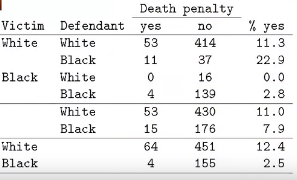
\includegraphics[scale=.8]{figs/data points_week4.png}
    \caption{Data Groups}
    \label{fig:Data Groups}
\end{figure}

By close inspection of the data we see that white defendants receive the death penalty a fewer percentage of the time, 11\% compared to 22\%, for both white and black victims. Zero of the white defendants received the death penalty whilst 2.8\% for the black victims. 

But, if we disregard the race of the victim, it turns out that white defendants receive the death penalty a greater percentage of the time, 11\% compared to 7.9\%. And if we look the race of the victim, disregarding the race of the defendant, actually in the instance where the victim was white, the defendant received the death penalty a higher percentage of the time, 12.4\% compared to a 2.5\%. 

In this setting, what would be the conclusion about death penalty verdicts vs. defendants and victim's race? A priori, we get two totally different and contradictory answers, depending if we're analysing the raw data itself or the marginal probabilities. Which one is the right answer? \\

Let's analyse the data:

\begin{itemize}
    \item Marginally, white defendants received the death penalty a greater percentage of the time than black defendants.
    \item Across white and black victims, black defendant's received the death penalty a greater percentage of the time than white defendants. 
\end{itemize}

Simpson's paradox refers to the fact that marginal and conditional associations can be opposing. The death penalty was enacted more often for the murder of a white victim than a black victim. Whites tend to kill whites (demographically), hence the larger marginal association. Thus, Simpson's paradox states that two variables can change when factoring a third variable\footnote{For further research, see Larry Wasserman's post "The normal deviate" on Simpson's Paradox.}. 

\subsubsection{Simpson's Paradox, more examples}

Consider now the following example. We're interested in comparing two player's batting averages. Let the data be 

\begin{figure}
    \centering
    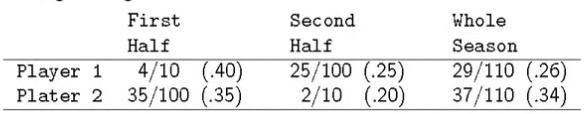
\includegraphics[scale=.5]{figs/data points_week4_part2.png}
    \caption{Caption}
    \label{fig: Data groups}
\end{figure}

Player 1 has a better batting average than Player 2 in both the first and second half of the season, yet has a worse batting average overall.  Player 1 had a very good batting average when they had relatively few bats and a modest batting average when they had lots of bats and vice-versa for player two. 

A famous example of Simpson's paradox is present in UC Berkeley Admissions data. We're given a certain dataset and and the total number of admitted and rejected applications for males and females, as it can be seen in \ref{fig: Data group ucb}.

\begin{figure}
    \centering
    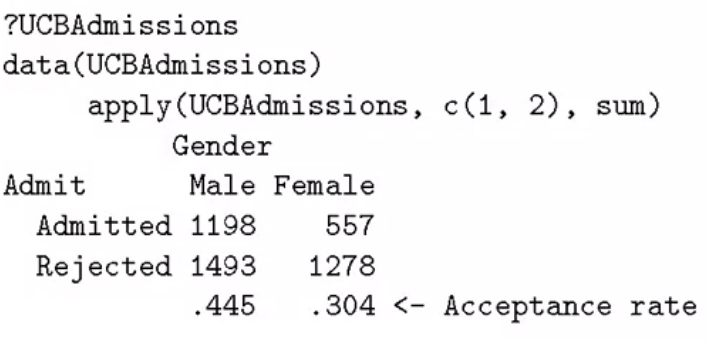
\includegraphics[scale=.5]{figs/data points_week4_part3.png}
    \caption{Berkeley Admissions data}
    \label{fig: Data group ucb}
\end{figure}

It turns out the male acceptance rate was higher than the females' acceptance rate, disregarding everything else. But if we study the acceptance rates by departments, it turns out that in almost every department, males had a lower acceptance rate than females. There are different gender acceptance rates by department. \\

Mathematically, Simpson's paradox is not paradoxical. Let $a,\cdots,h \in \mathds{Z}$, then 

\begin{align*}
   \textnormal{if } a/b < c/d \textnormal{ and } e/f < g/h \Rightarrow (a+e)/(b+f) > (c+g)/(d+h)
\end{align*}

In statistical terms, it says that the apparent relationship between two random variables can change in the light or absence of a third random variable. It's only when we conflate the probabilistic statements and the evidence associated with probabilistic statements, vis a vie the data, with the causal statements, that so-called paradoxes may arise. In general, it's a non-trivial problem to determine how much conditioning is enough on a given dataset so as to extract reliable conclusion. This problem of confounding is treated by the Causal inference sub-discipline.  

\subsubsection{Weighting and Confounding}

Variable that are correlated with the explanatory and response variables can distort the estimated effect. In our previous example, victim's race was clearly correlated with the defendant's race and the death penalty verdict. With a confounder present, we're not able to distinguish an event being causally related with race in the death penalty experiment versus something that has a statistical association with race and death penalty verdict. We're interested in events or random variables which have a statistical association with the explanatory and response variables, where there is a plausible causal connection between them. 

Let's assume we have a single confounder. How do we deal with it? One way is with regression, whilst another strategy in categorical data analysis to adjust for confounding variables is to stratify by the confounder and then combine the strata-specific estimates. This requires appropriately weighting the strata-specific estimates. Note that unnecessary stratification reduces precision. \\

Suppose we have two unbiased scales, one with a variance of 1lb and the other one with variance of 9lbs. Confronted with weights from both scales, would you give both measurements equal creedance?

Suppose that we weigh a certain object with the first scale. This is represented by a random variable which we assume to be normal, $X_1 \sim \mathcal{N}(\mu, \sigma_1^2)$. Similarly, weighing this object in the second scales gives another random variable which we assume to be normal as well, $X_2 \sim \mathcal{N}(\mu, \sigma_2^2)$. Note that both $\sigma_1$ and $\sigma_2$ are known. We'd like to estimate $\mu$, then the log-likelihood for $\mu$ is 

$$
-\frac{(x_1-\mu)^2}{2\sigma_1^2}-\frac{(x_2-\mu)^2}{2\sigma_2^2} + \cdots,
$$

where the dots stand for terms which don't depend on $\mu$. We take the derivative with respect to $\mu$ and we set it to zero:

\begin{align*}
-\frac{(x_1-\mu)}{\sigma_1^2}-\frac{(x_2-\mu)}{\sigma_2^2} = 0 \\
\Rightarrow\frac{x_1r_1+x_2r_2}{r_1+r_2} = x_1 p_1 + x_2(1-p),
\end{align*}

where $r_i = \frac{1}{\sigma_i^2}$ and $p = \frac{r_1}{r_1+r_2}$. Note that if $X_1$ has very low variance, then its term dominates the estimate for $\mu$. The general principle thus being: instead of averaging over several unbiased estimates, take a single average weighted according to the inverse variances. In our example, $\sigma_1^2 =1$,  $\sigma_2^2 =9$ so $p=.9$.  

\subsubsection{C Mantel Haenszel Estimator and Test}

Consider the death penalty statistical trial. We have two two-by-two tables, were we are given the data of the defendant's race and whether or nor they got a death penalty verdict and then we stratified that by a third random variable, the victim's race. Thus, let $n_{ijk}$ be the $ij$th-entry of the $k$th-table. In other words, $k=1$ is the first victim's race, $k=2$ is the second victim's race and so on, then $i$ and $j$ would index defendant's race and whether or not the person got the death penalty. The $k$th-sample odds ratio (main diagonal elements divided by the off-diagonal elements) is given by 

$$
\hat{\theta}_k = \frac{n_{11k}n_{22k}}{n_{12k}n_{21k}},
$$

The Mantel Haenszel estimator is the weighted average of these strata-specific estimates and is given by

\begin{align*}
    \hat{\theta} = \frac{\sum_{k}r_{k}\hat{\theta}_k}{\sum_{k}r_{k}}\textnormal{ where the weights are } r_k = \frac{n_{12k}n_{21k}}{n_{++k}},
\end{align*}

this is, in essence, a simplicial convex combination of the strata-specific odds ratios. The weights are in essence inverse variances of hypergeometric distributions. The estimator simplifies to\footnote{
The standard error can be found in Agresti (page 235) or Rosner (page 656)} 

$$
\hat{\theta}_{MH} = \frac{\sum_{k}\frac{n_{11k}n_{22k}}{n_{++k}}}{\sum_{k}\frac{ n_{12k}n_{21k}}{n_{++k}}}.
$$

Let's now consider the following example of a medication's medical trial with the dataset given in \ref{fig: CMH test}. Let T be the active drug, C the placebo, S stands for success and F for failure. We're interested in whatever policies and practices existed at the various centers at which the data was collected by the means of a center-stratification with 8 strata. Then we have eight odds ratio and we wish to analyse if the center, as a random variable, was a confound. 

\begin{figure}
    \centering
    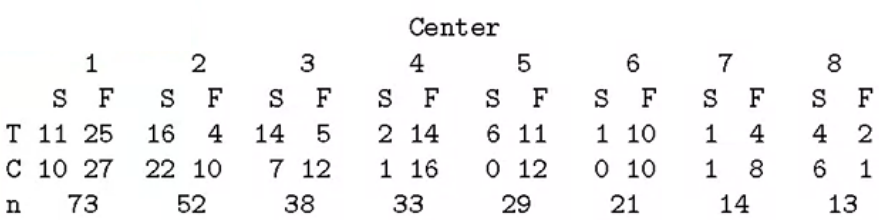
\includegraphics[scale=0.5]{figs/data points_week4_part4.png}
    \caption{Dataset for a medical trial in the context of a CMH test.}
    \label{fig: CMH test}
\end{figure}

Let's first imagine if the center was specifically associated with the treatment application (some centers tended to apply the treatment more than others) and that the center was associated with the success of the treatment due to different policies. In order to gain insight, we stratify by center, obtain a strata-specific odds ratio and then factoring in the inverse variance of the odds ratios (since some centers have more patients than others). For example, center 1, with 73 test subjects, has more weight in the final result than center 7, which only has 14 test subjects; since the first center has a better, more precise, odds ratio. Therefore, the Mantel Haenszel estimate is 

$$
\theta_{MH} = \frac{(11 \times 27)/73+(16 \times 10)/25+ \cdots + (4 \times 1)/13}{(10 \times 25)/73+(4 \times 22)/25+\cdots +(6 \times 2)/13} = 2.13,
$$

also $\log \theta_{MH} = .758$ and $\hat{SE}_{\log \theta_{MH}} = .303$. 

Another rationale for a stratified-estimate, is that we're under the impression that the center is at some level, a random effect, and is a modifier for the treatment. The centers studied are a random draw from the population of centers, and since we're not interested in a given center's specific (ie. we don't care if treatment worked at center number 1 or not), we care only if it worked overall. Therefore a CMH test is an average over a certain number of random draws from a given population of centers and quantifies it's effect on the treatment. This is called \underline{common odds ratio across centers}.\\

Now, we're interested in testing if the common odds ratios are equal to 1. Let $\theta_i$ be the $i$th-strata-specific odds ratio, then let $H_0 : \theta_1 = \cdots=\theta_k = 1$ versus the alternative $H_a : \theta_1 = \cdots=\theta_k \neq 1.$ The CMH test does apply to the other alternatives but it works best for the previous alternative hypothesis. This test is, in essence, the same as the test for conditional independence of response and exposure given the stratifying variable. In the Cochran Mantel Haenszel test is executed by conditioning on the rows (similarly as Fisher's exact test) and columns for each of the $k$ contingency tables, resulting in $k$ hypergeometric distributions and leaving only the $n_{11k}$ cells free. Under the conditioning and under the null hypothesis, 

\begin{align*}
    \mathds{E}(n_{11k}) = \frac{n_{1+k}n_{+1k}}{n_{++k}} \textnormal{ and } \mathds{V}\textnormal{ar}(n_{11k}) = \frac{n_{1+k}n_{2+k}n_{+1k}n_{+2k}}{n_{++k}^2(n_{++k}-1)}.
\end{align*}

Then the CMH test statistic is 
$$
\frac{[\sum_{k}(n_{11k}-\mathds{E}(n_{1+k}))^2]}{\sum_{k} \mathds{V}\textnormal{ar}(n_{11k})},
$$

the sum of the deviations of the upper left-hand cells from their expected values, summed up. Contrast this to the chi-squared test, where they are first squared and then summed up. For many large sample sizes and under the null hypothesis, this test statistic is $\chi^2(1)$, regardless of how many table are being summed up. Remember that the CMH test is used when we're interested in analysing whether or not the odds ratio is one, given that it's common across all strata. An CMH can be performed in R using the following R routine

\begin{lstlisting}[language=R]
dat <- array(c(11, 10, 25, 27,  16, 22,  4, 10,
               14,  7,  5, 12,   2,  1, 14, 16,
                6,  0, 11, 12,   1,  0, 10, 10,
                1,  1,  4,  8,   4,  6,  2,  1),
             c(2,2,8))
mantelhaen.test(dat, correct=FALSE)

In [1]: Mantel-Haenszel chi-squared test without continuity correction

In [2]: data:  dat
In [3]: Mantel-Haenszel X-squared = 6.3841, df = 1, p-value = 0.01151
In [4]: alternative hypothesis: true common odds ratio is not equal to 1
In [5]: 95 percent confidence interval:
In [6]: 1.177590 3.869174
In [7]: sample estimates:
In [8]: common odds ratio 
In [9]:         2.134549
\end{lstlisting}

The result for the CMH test statistic is 6.38 and we'll compare this to $\chi^2(1)$ value and we're going to reject for larger values. Since the P-value is $0.012$ the CMH test suggest that the treatment and response are not conditionally independent given center. \\

It's possible to perform an analogous test in a random effects logit model that benefits from a complete model specification. It's also possible to test heterogeneity of the strata-specific odds radio. It's also possible to test if all the odds ratios are equal by the means of a Wolffe's tests. Note that exact test, which guarantee the type I error rate, are also possible in R by the means of the \texttt{exact = TRUE} command. 

\subsubsection{Case Control Sampling}

In this section, we're going to treat case control methods, the instance where using using retrospective case control data and a so called rare disease assumption, we can estimate prospective odds ratios; and finally the exact inference for odds ratios. \\

Let's start by studying retrospective in reference sampling. We're interested in studying lung cancer cases and controls and to ascertain whether or not they were a smoker. There are two ways to collect this data: we could follow a given number of test subjects over time, some of them would smoke, and some of then wouldn't, and then we could quantify the amount of positive lung cancer diagnosis. This sampling method is inadequate and impossible for large sample sizes. Another form to obtain this data would be by finding a given number of positive lung cancer patients and find the same number of controls, at some level comparable to the first group. And the we'd retrospectively determine whether or not they were smokers. The margins for both groups are fixed (both are 709). In case-control studies, it's also the norm to find a control which very closely matches a specific case and repeat this procedure for all cases. 
Let the data be given by the following table

\begin{center}
Table 1 = 
\begin{tabular}{ |c|c|c|c| } 
& Lung cancer & \\
\hline
Smoker & Cases & Controls & Total \\
\hline
Yes & 688 & 650 & 1338 \\ 
No & 21 & 59 & 80\\  
\hline 
& 709 & 709 & 1418
\end{tabular}
\end{center}

We're interested in ascertaining who is a smoker and whether or not the cases group had a greater proportion of smokers and to make prospective conclusions to this retrospective data. It's impossible to directly estimate $\mathds{P}(\textnormal{Case}|\textnormal{Smoker})$, but it's possible to estimate $\mathds{P}(\textnormal{Smoker}|\textnormal{Case})$ given the data. We can also estimate the odds ratios in particular, we're interested in the odds of being a case given that the test subject is a smoker relative to the odds of becoming a case given that the test subject is a non-smoker. But this is equivalent to finding the odds of being a smoker given that the test subject is a case relative to the odds of being a smoker given that the test subject is a case. This is

$$
\frac{Odds(\textnormal{Case}|\textnormal{Smoker})}{Odds(\textnormal{Case}|\textnormal{Smoker}^c)} = \frac{Odds(\textnormal{Smoker}|\textnormal{case})}{Odds(\textnormal{Smoker}|\textnormal{case}^c)}.
$$

Let $C$ stand for Case, and $S$ for smoker, then

\begin{align*}
    \frac{Odds(\textnormal{Case}|\textnormal{Smoker})}{Odds(\textnormal{Case}|\textnormal{Smoker}^c)} &=\frac{\mathds{P}(C|S)/\mathds{P}(\bar{C}|S)}{{\mathds{P}(C|\bar{S})/\mathds{P}(\bar{C}|\bar{S})}} = \frac{\mathds{P}(C, S)/\mathds{P}(\bar{C}, S)}{{\mathds{P}(C, \bar{S})/\mathds{P}(\bar{C}, \bar{S})}}\\
    &=\frac{\mathds{P}(C, S)\mathds{P}(\bar{C}, \bar{S})}{{\mathds{P}(C, \bar{S})\mathds{P}(\bar{C}, {S})}},
\end{align*}

which is the probability of caseness and smokerness times by the probability of being neither a case nor a smoker divided by the product of the off-diagonal probabilities. Note that
by exchanging $C$ and $S$ we get the same result since $\mathds{P}(A,B)=\mathds{P}(B,A)$. 

Remember that the sample odds ratio is $\frac{n_{11}n_{22}}{n_{12}n_{21}}$, which remains unchanged if a row or column is multiplied by a constants, and is transpose-invariant (the odds ratio do not change by changing which factor is the outcome and which factor is the predictor). \\

Now, it turns out that the odds ratio is related to the relative risk. In effect

\begin{align*}
    OR &= \frac{\mathds{P}(S|C)/\mathds{P}(\bar{S}|C)}{{\mathds{P}(S|\bar{C})/\mathds{P}(\bar{S}|\bar{C})}} \\
    &= \frac{\mathds{P}(C|S)/\mathds{P}(\bar{C}|S)}{{\mathds{P}(C|\bar{S})/\mathds{P}(\bar{C}|\bar{S})}} \\
    &= \frac{\mathds{P}(C|S)}{\mathds{P}(C|\bar{S})} \frac{\mathds{P}(\bar{C}|\bar{S})}{\mathds{P}(\bar{C}|S)}\\
    &= RR \times \frac{1- \mathds{P}(C | \bar{S})}{1- \mathds{P}(C | {S})} \textnormal{ where } RR =   \frac{\mathds{P}(C|S)}{\mathds{P}(C|\bar{S})}
\end{align*}

where in line 2 we reversed the odds ratio. Note that the odds ratio aproximates the relative risk if $\mathds{P}(\bar{C}|\bar{S})$ and $\mathds{P}(C|\bar{S})$ are nearly equal or very small. This is case when the case-ness is very small ie. regardless of whether a test subject smokes or not, the probability of lung cancer is very small. This is the case of the \textbf{rare disease assumption} which implies $OR \approx RR$. It's important to clarify that, for the rare disease assumption to be valid, it has to be rare among the exposed and non-exposed both, not rare overall.

Consider the following example 

\begin{tcolorbox}[title=Example of Rare Disease Assumption]

Let the data be given by the following table

\begin{center}
Table 2 = 
\begin{tabular}{ |c|c|c|c| } 
& Disease & \\
\hline
Exposure & Yes & No & Total \\
\hline
Yes & 9 & 1 & 10 \\ 
No & 1 & 999 & 1000\\  
\hline 
& 10 & 1000 & 1010
\end{tabular}
\end{center}

The estimated probability of the disease is $\hat{\mathds{P}}(D) = \frac{10}{1010}\approx .01$, the odds ratios is $\hat{OR}=\frac{9\times 999}{1 \times 1} = 8991$, $\hat{RR}=\frac{9/10}{1/1000} = 900$. Disease is rare overall but it's not rare among the exposed which explains why the odds ratio doesn't approximate the relative risk. 
\end{tcolorbox}

Let's do a recap:

\begin{itemize}
    \item $OR=1$ implies no association between the data, 
    \item $OR >1$ implies a positive association
    \item whilst $OR < 1$ implies a negative association. 
    \item For retrospective case control studies, the odds ratio can be interpreted prospectively.
    \item For diseases rare among both the case and control groups, the odds ratio approximate the relative risk.
    \item The delta method gives the standard error for the logarithm of the odds ratio as 
    $$
    \sqrt{\frac{1}{n_{11}}+\frac{1}{n_{12}}+\frac{1}{n_{21}}+\frac{1}{n_{22}}}
    $$
\end{itemize}

Going back to table 1 and the lung cancer example we have that the estimated odds ratio is $\hat{OR}= \frac{688 \times 59}{21 \times 650} = 3.0$, the estimated standard error for the logarithm of the estimated odds ratio is 

$$
\hat{SE}_{\log \hat{OR}} = \sqrt{\frac{1}{688}+\frac{1}{650}+\frac{1}{21}+\frac{1}{59}} = .26.
$$

The confidence interval at 95\% confidence is $CI= \log(3.0) \pm 1.96 \times .26 = [.59, 1.61]$.

Note that the estimated odds of lung cancer for smokers is three times that of the odds for non-smokers with an interval of [exp(.59), exp(1.61)] = [1.80, 5.00] \footnote{For further research, look up \url{https://www.bayesrulesbook.com/chapter-1.html}}.

\subsubsection{Exact inference for the Odds Ratio}

Let $X$ be the number of smokers for the cases and $Y$ be the number of smokers for the controls. The margins are fixed and $X$ and $Y$ are random numbers modelled as binomial distributions. We desire to calculate an exact confidence interval for the odds ratio. In order to do that, first we need to eliminate the nuisance parameter. 

Let $\textnormal{logit}(p)=\log\frac{p}{1-p}$ be the log-odds. The differences in logits are the log-odds ratios ($\textnormal{logit}(p_1) -\textnormal{logit}(p_2) = \textnormal{logit}(p_1/p_2) $.

\begin{align*}
   & \textnormal{If } \textnormal{logit}(\mathds{P}(\textnormal{Smoker}|\textnormal{Case}))=\delta \textnormal{ then }\mathds{P}(\textnormal{Smoker}|\textnormal{Case}) =\frac{e^{\delta}}{1+e^{\delta}}, \\
   &\textnormal{If } \textnormal{logit}(\mathds{P}(\textnormal{Smoker}|\textnormal{Control}))=\delta + \theta \textnormal{ then }\mathds{P}(\textnormal{Smoker}|\textnormal{Control}) =\frac{e^{\delta+ \theta}}{1+e^{\delta+ \theta}},
\end{align*}

where $\theta$ is the log-odds ratio and $\delta \in \mathds{R}$ is the nuisance parameter, which we wish to eliminate. If $X \sim \textnormal{Binom}\bigg(n_1, p_1 = \frac{e^{\delta}}{1+e^{\delta}}\bigg)$ and if $Y \sim \textnormal{Binom}\bigg(n_2, p_2 = \frac{e^{\delta+ \theta}}{1+e^{\delta+ \theta}}\bigg)$, then 

\begin{align*}
\mathds{P}(X = x) &= {{n_1}\choose{x}} \bigg( \frac{e^{\delta}}{1+e^{\delta}}\bigg)^x\bigg( \frac{1}{1+e^{\delta}}\bigg)^{n_1-x} \\
&= {{n_1}\choose{x}} e^{x\delta} \bigg( \frac{1}{1+e^{\delta}}\bigg)^{n_1}.
\end{align*}

Then 

\begin{align*}
   \mathds{P}(Y = z-x) &=  {{n_2}\choose{z-x}} e^{(z-x)\delta+(z-x)\theta}\bigg( \frac{1}{1+e^{\delta+\theta}}\bigg)^{n_2}.
\end{align*}

Thus, since $X$ and $Y$ are not identically distributed we have 

\begin{align*}
    \mathds{P}(X+Y = z) = \sum_{u} \mathds{P}(X=u) \mathds{P}(Y=z-u).
\end{align*}

Finally, the probability that the random variable $X$ takes a particular value $x$ given that the sum of random variables $X+Y$ takes on a particular value $z$ is 

\begin{align*}
    \mathds{P}(X=x | X+Y = z; \theta) &= \frac{\mathds{P}(X=x)\mathds{P}(Y=z-x)}{\sum_{u}\mathds{P}(X=u)\mathds{P}(Y=z-u)} \\
    &= \frac{{{n_1}\choose{x}}{{n_2}\choose{z-x}}e^{x\theta}}{\sum_{u}{{n_1}\choose{u}}{{n_2}\choose{z-u}}e^{u\theta}},
\end{align*}

this distribution is so called the non-central hypergeometric distribution, where $\theta$ is the log odds ratio\footnote{Note this test is similar to Fisher's exact test but the difference lies in that we haven't assumed the null hypothesis to be true and depends on $\theta$.} and it doesn't depend on $\delta$ (we've conditioned on $X+Y$ and eliminated the nuisance parameter). This distribution can then be used to calculate exact hypothesis tests for $H_0: \theta = \theta_0$. Inverting said exact test yields the exact confidence interval for the odds ratio. Note that this distribution simplifies to the hypergeometric distribution for $\theta = 0$ and the test is none other than Fisher's exact test. The R-routine \texttt{Fisher.test} performs this calculation. 

\subsubsection{Matched 2x2 Tables}

We're now interested in treating matched two-by-two tables, which are similar in nature to paired $T$-tests but with binary data, the subject of dependence and the relationship to the CMH test. \\


We're interested in studying the approval and disapproval rates of a politician on two occasions. The dataset is given in \ref{fig:dataset5}.

\begin{figure}
    \centering
    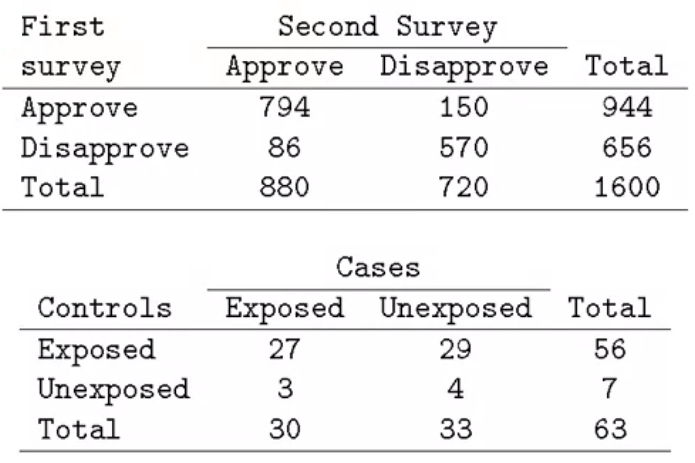
\includegraphics[scale=.5]{figs/data points_week4_part5.png}
    \caption{Matched 2x2 tables Example from Agresti's book}
    \label{fig:dataset5}
\end{figure}

In this case, 749 had the same positive opinion in both surveys and 150 approved the first time and disapproved the second time. This example can be though as a retrospective case-control test. 

\subsubsection{Dependence and Marginal Homogeneity}

Matched binary data can arise from 

\begin{itemize}
    \item Measuring a response at two occasions, 
    \item matching on case status in a retrospective study,
    \item or by matching on exposure status in a prospective or cross-sectional study.
\end{itemize}

Matching in general induces dependence which need to be accounted for in the analysis. 
The pairs on binary observations are dependent, so our existing methods are no longer applicable. We'll discuss the process of making conclusions about the marginal probabilities and odds. We'll assume independence across pairs and dependence within pairs. 

Let's consider a general example for matched tables and notations. Consider figure \ref{fig:notations} and the standard contigency table notation given in table 1.  

\begin{figure}
    \centering
    \includegraphics[scale=0.5]{figs/data points_week4_part6.png}
    \caption{Notation convention for matched 2x2 tables.}
    \label{fig:notations}
\end{figure}

We assume that $(n_{11},n_{12}, n_{21},n_{22})$ are multinomial with $n$ trials and success probabilities $(\pi_{11},\pi_{12},\pi_{21},\pi_{22})$ respectively. This is, every time 1-time 2 collection pair of measurements, is going to be a one or a zero in exactly in one of these four locations. So the person will have either said yes at both occasions, a yes and no, a no and a yes or no at both occasions. The probability of being a one in the $ij$th-cell is $\pi_{ij}$. Note that $\pi_{1+}$ and $\pi_{+1}$ are the marginal probabilities of a yes response at the two occasions, this is $\pi_{1+} = \mathds{P}(\textnormal{Yes}|\textnormal{Time 1})$ (regardless of Time 2's results) and $\pi_{+1} = \mathds{P}(\textnormal{Yes}|\textnormal{Time 2})$ (regardless of Test 1's results). Similarly for the second set of $\pi_2$.\\

We define marginal homogeneity is the hypothesis $H_0: \pi_{1+}=\pi_{+1}$ which is equivalent to the (transpose) symmetry of the off-diagonal elements $H_0: \pi_{12}=\pi_{21}$\footnote{This statement is only true for 2-by-2 tables and doesn't stand for more general cases.}. The obvious estimate for $\pi_{12}-\pi_{21}$ is 

$$
\frac{n_{12}}{n} - \frac{n_{21}}{n},
$$

which quantifies how far away from symmetry the data is ie. how far away from marginal homogeneity the data is. 
Note that under the null hypothesis, a consistent estimate of the variance is $
\frac{n_{12}+n_{21}}{n^2}.$

Therefore the $z$-statistic is the previous estimate divided by the standard error ie. 

$$
\frac{(n_{12}-n_{21})^2}{n_{12}+n_{21}} \underset{\textnormal{asymp.}}{\sim} \chi^2_{1}.
$$

This is the so-called \textbf{McNemar's test statistic}, and we reject the null hypothesis if the test statistic is large. Notice only discordant cells enter into the test, both $n_{12}$
and $n_{21}$ carry the relevant information about whether or nor $\pi_{1+}$ and $\pi_{+1}$ differ. Notice $n_{11}$ and $n_{22}$ contribute information to estimating the magnitude of this difference. \\

Consider the approval rating example. In that case, we have $86$ and $150$ as the off-diagonal cells, then the test statistic is $\frac{(86-150)^2}{86+150} = 17.36$, with a P-value of $3\times 10^{-5}$. Hence, we reject the null hypothesis and conclude there is evidence to suggest a change in opinion between the two polls. This test can be performed via the following R routine

\begin{lstlisting}[language=R]
mcnemar.test(matrix(c(794, 86, 150, 570), 2),
             correct=FALSE)
\end{lstlisting}

which doesn't applies a continuity correction. \\

\subsubsection{Estimation of the Marginal Difference in Proportions}

We'd also like to construct a confidence interval for our test. Let $\hat{\pi}_{ij} = \frac{n_{ij}}{n}$ be the estimated sample proportions and we're interested in estimating $d = \hat{\pi}_{1+}-\hat{\pi}_{+1}= \frac{n_{12}-n_{21}}{n}$, the difference in marginal proportions. The variance of $d$, in general (needing not the null hypothesis to be true) is 

$$
\sigma^2_d = \frac{1}{n} \times \bigg[{\pi}_{1+}(1-{\pi}_{1+})+{\pi}_{+1}(1-{\pi}_{+1})-2({\pi}_{11}{\pi}_{22}-{\pi}_{12}{\pi}_{21})\bigg],
$$

where the last term accounts for the correlation in the dataset, where $\frac{d-({\pi}_{1+}-{\pi}_{+1})}{\hat{\sigma}_d} \underset{\textnormal{asymp.}}{\sim} \mathcal{N}(0,1)$, from where it's trivial to construct the confidence interval. \\

We could also compare $\sigma_d^2$ with what we would use if the proportions were independent, this is: instead of asking the same test subjects on two occasion whether or not they approve, what if we tested a different set of people each time? it would be logical to think that people who approved on the first occasion, would be more likely to approve on the second occasion, and the same logic applies to disapproval rates; the measurements tend to be concordant. This happens when ${\pi}_{11}{\pi}_{22} > {\pi}_{12}{\pi}_{21}$, tending to lie on the main diagonal, which implies a dramatic reduction in the variance. Failing to account for the fact that the same people were asked twice, would imply a much wider, less precise, confidence interval. 

\subsubsection{Odds and Ends for Matched 2x2 Tables}

Now, let's go through our example:

\begin{itemize}
    \item the difference in marginal proportions is $d= \frac{944}{1600}-\frac{880}{1600} = .59 - .55 = .04$,
    \item $\hat{\pi}_{11}=.50$, $\hat{\pi}_{12}=.09$, $\hat{\pi}_{21}=.05$, $\hat{\pi}_{22}=.36$, 
    \item $\hat{\sigma}_d^2 = \frac{.59(1-.59)+.55(1-.55) - 2\times(.50 \times .36 - .09 \times .05}{1600}$, thus $\hat{\sigma}_d = .0095$.
    \item $95\% CI = .04 \pm 1.96 \times 0.095 = [.06, .02]$.
\end{itemize}

Note that ignoring dependence would yield $\hat{\sigma}_d = .0175$, giving a lower performing confidence interval. \\

There's a non-trivial relationship to the Cochran-Mantel-Haenszel test and the matched 2-by-2 tables. Consider the situation in which we take each pair and represented their time, first and second, and report their responses, either a yes or a no. This can be thought as an extremely stratified setting where every strata has the two measurements. Doing this leaves only four possible tables, pictured in \ref{fig:matched-2x2-cmh}. These tables will exactly reproduce the two-by-two table. 

\begin{figure}
    \centering
    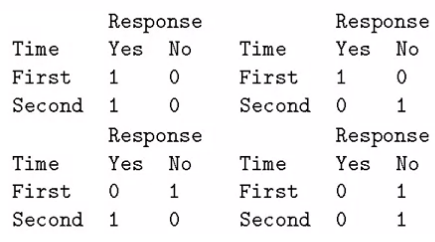
\includegraphics{figs/data points_week4_part7.png}
    \caption[scale=.5]{Relationship to the Cochran-Mantel-Haenszel test.}
    \label{fig:matched-2x2-cmh}
\end{figure}

The McNemar's test is equivalent to the CMH test where subject is the stratifying variable and each 2$\times$2 table is the observed zero-one table for that subject. This is useful only as a theoretical justification. Performing the CMH test on these heavily-stratified dataset, the tables, with the stratifying variable being the subjects results in McNemar's test. \\

McNemar's test has an exact version. Consider the off-diagonal cells, $n_{12}$ and $n_{21}$. Under the null hypothesis $H_0 : \frac{\pi_{12}}{\pi_{12}+\pi_{21}} = .5$. Therefore, under $H_0$, $n_{21} |n_{12}+n_{21}$ is binomial with success probability $.5$ and $n_{12}+n_{21}$ trials. We can use this result to construct an exact P-value for matched pairs data. Under the null hypothesis, the two off-diagonal probabilities are identical. Landing on either of the off-diagonal cells is a fair coin-toss for every matched pair. We'd have evidence against $H_0$ if the said number of trials were not equal. This is related to the \textbf{non-parametric sine test}, under the null hypothesis, results should exchangeable whether they agree in terms of approving and disapproving or disapproving and approving. 

Consider the approval rating data. Let $H_0 : \pi_{21}=\pi_{12}$ versus the alternative $H_a: \pi_{21} < \pi_{12} \equiv \pi_{+1}<\pi_{1+}$, where $\pi_{+1}$ is the approval at time 2 disregarding time 1 whilst $\pi_{1+}$ is the approval at time 1 disregarding time 2. We're testing if the approval at time 2 is lower that the approval at time 1. 86 people disapproved on the first survey and approved on the second survey ($n_{21}$ cell). In particular, we're going to test if that is smaller than what would be expected by chance and find the probability of getting data as or more extreme in favour of the alternative case: $\mathds{P}(X \leq 86 |86 + 150) = .0 \textnormal{ where } X\sim \textnormal{Bin}(p=.5, n=236).$ We then reject the null hypothesis. For two sided tests, we can double the smaller of the two one-sided tests. \\

The marginal odds ratio is the odds of approval at time 1 relative to the odds of approval at time 2:

$$
\frac{\pi_{1+}/\pi_{2+}}{\pi_{+1}/\pi_{+2}} = \frac{\pi_{1+}\pi_{+2}}{\pi_{+1}\pi_{2+}}.
$$

which is the quotient of the odds of approval at time 1 divided by the odds of approval at time 2 in the denominator, its a marginal odds ratio since we're dealing with marginal probabilities. Note this is in essence a paired-group test since the same sample group was tested twice. 
The maximum likelihood estimate of the marginal log odds ratio is 

$$
\hat{\theta} = \log \frac{\pi_{1+}\pi_{+2}}{\pi_{+1}\pi_{2+}},
$$

and the asymptotic variance of this estimator is 

$$
\frac{1}{\pi_{1+}\pi_{2+}} + \frac{1}{\pi_{+1}\pi_{+2}} - 2\frac{(\pi_{11}\pi_{22}-\pi_{12}\pi_{21})/(\pi_{1+}\pi_{2+}\pi_{+1})\pi_{+2}}{n},
$$

which can then be used to calculate a confidence interval for a two by two dataset. 

In the approval rating example, the marginal OR compares the odds of approval at time 1 to that at time 2. Then $\hat{\theta}= \log(944\times 720/(880\times656)) = .16$, with an estimated standard error of $.039$. Therefore the confidence interval for the log odds ratio is $.16 \pm 1.96 \times .039 = [.084, .236]$. \\

Let's imagine if we created a logit model for our approval rating data. 

\begin{align*}
   & \textnormal{logit}(\mathds{P}(\textnormal{Person } i \textnormal{ says Yes at Time 1}) = \alpha + U_i \\
    & \textnormal{logit}(\mathds{P}(\textnormal{Person } i \textnormal{ says Yes at Time 2}) = \alpha + \gamma + U_i,
\end{align*}

where each $U_i$ contains person-specific random effects. A person with a large $U_i$ is likely to answer Yes at both occasions, where $\gamma$ is the \textbf{log odds ratio} comparing a response of Yes at Time 1 to a response of Yes at Time 2, which is a subject specific effect. If we subtract the log odds of a yes responde for two different people, the $U_i$ terms wouldn't cancel. One way to eliminate $U_i$ is to perform a conditional estimate, and to condition on the total number of Yes responses for each person: 1. if they answered yes or no on both ocassion then you know both responses, therefore only discordant pairs have any relevant information after conditioning. Therefore, the conditional ML estimate for $\gamma$ and its standard error are

\begin{align*}
    \log \frac{n_{21}}{n_{12}} & \sqrt{\frac{1}{n_{21}}+\frac{1}{n_{21}}}.  
\end{align*}

The marginal ML has a marginal interpretation. The effect is averaged over all of the values of $U_i$. The conditional ML estimate has a subject specific interpretation. Marginal interpretations are in general more useful for policy type statements. Policy makers tend to be interested in how factors influence populations. Subject specific interpretations are more useful in clinical applications. Physicians are interested in how many factor influence the individuals. 

\subsubsection{The Sign Test}

In this section we'll treat some non-parametric tests, which include the sign test, the signed rank test (useful for paired tests),  Monte-Carlo simulations of said test, independent groups, the Mann-Whitney test and their relationship to permutation tests. \\

In general, distribution-free methods require fewer assumptions than parametric methods. In said types of test, the focus is on testing rather than estimation and are not sensitive to outlying observation. These are specially suited to analyse cruder data, like ranks, and discard some of the information in the data, which is a downside. Therefore they may be less powerful than parametric counterparts, even when the parametric assumptions are true. For large-enough samples, they are equally efficient to parametric counterparts. 

Consider the following example, where 25 fish were tested at two locations for their mercury levels in parts per million. 

\begin{figure}
    \centering
    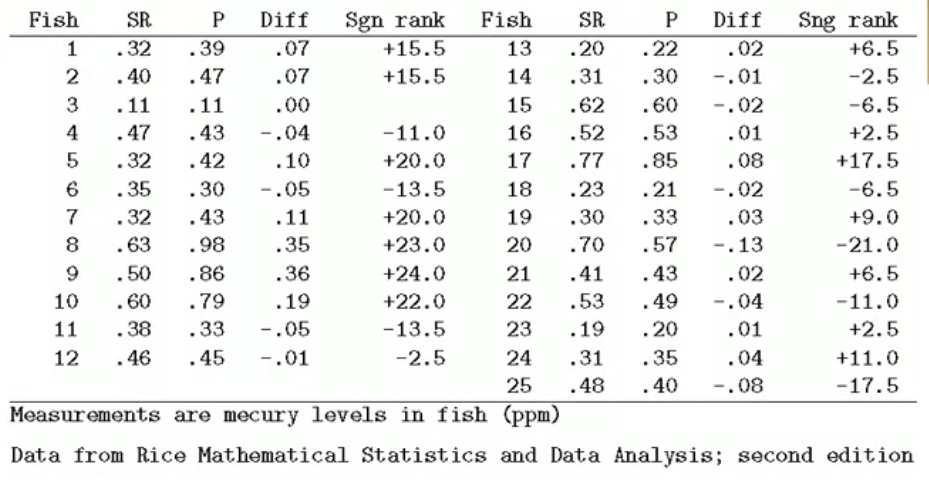
\includegraphics[scale=.5]{figs/data points_week4_part8.png}
    \caption{Dataset for the Sign test.}
    \label{fig: sign test}
\end{figure}

In this dataset, since the same fish were tested at two different locations, each fish serves as its own control. Therefore with a non-parametric test we're interested in analysing the validity of the assumptions, such as normality. 

Let $D_i = \textnormal{difference} (P-SR)$, let $\theta$ be the population median of the difference $D_i$. The null hypothesis is $H_0: \theta = 0$ versus $H_a: \theta \neq 0$, or one of the other two alternatives. By definition of the median, $\theta=0$ if and only if $p = \mathds{P}(D>0)=.5$.
Assuming iid data, let $X$ be the number of times $D>0$ which in turn implies $X\sim \textnormal{Binom}(n,p)$. The sign tests whether $H_0: p=.5$ using X, if $X$ is excessively large or excessively small, this would dispute the null hypothesis, by performing an exact binomial test.\\

Consider the previous example. Let $\theta = \textnormal{median difference } p - sr$, with the null hypothesis being $H_0: \theta = 0$ versus the alternative hypothesis being  $H_a: \theta \neq 0$. The number of instances where the difference is bigger than 0 is 15 out 25 trials. From the R-function, we can test if 15 out 25 trials is excessively larger than 12.5 \texttt{binom.test(15,25)} which gives the \texttt{p-value = .4244}, thus there's a 42\% chance of happening under the null hypothesis for a two sided test. Or we could have used large sample tests for a binomial proportion:

\begin{lstlisting}[language=R]
prop.test(15, 25, p=.5)
X-squared = .64, df = 1, p-value = 0.4237
\end{lstlisting}

In essence this test analyses if levels of one data group are higher than the levels of the other group, by counting the number of pairs from the matched pairs where it's higher and by quantifying if this number is excessively large relative to a coin flip for each pair.\\

The only assumption made on the data is that the data-points are iid. There are some problems with these kind of problems. The magnitude of the difference itself is discarded, perhaps too much information being lost in the process. 
We could easily test $H_0: \theta=\theta_0$, for any value of $\theta_0$, by calculating the number of times $D>\theta_0$ and performing a binomial test. We can invert these test to get a distribution free confidence interval for the median. 

\subsubsection{The Sign Rank Test}

The main issue with the sign test is that the magnitude of differences is discarded, the test potentially not being as powerful as other techniques. \\

Wilcoxon treated the problem of discarding the magnitude of the differences by creating a test statistic which also takes into account the signed ranks of the differences, saving some of the information regarding the magnitude of the differences. The null hypothesis $H_0: \theta = 0$ is thus tested against one of the three alternatives. Appropriately normalised, the test statistic follows a normal distribution. Also note the exact small sample distribution of the signed rank statistic is known if there are no ties. With this test we can quantise how "normal" our distribution is. The signed rank procedure can be implemented as follows:

\begin{itemize}
    \item Take the paired differences, 
    \item take the absolute values of the differences, \item rank these absolute values and throwing away the zeros (throwing away the ties).
    \item Then, multiply the ranks by the sign of the difference, 
    \item and calculate the rank sum $W_+$ of the positive ranks
\end{itemize}

Therefore, remembering $\theta$ is the median,

\begin{itemize}
    \item If $\theta > 0$, then $W_+$ should be large.
    \item If $\theta < 0$ then $W_+$ should be small.
\end{itemize}

Properly normalized $W_+ \sim \mathcal{N}(\mu, \sigma^2)$ for some $\mu, \sigma \in \mathds{R}$. For small sample sizes $W_+$ has an exact distribution under the null hypothesis, being able to extract critical values from standardises tables.\\

This test can be performed with Monte Carlo simulations by simulating $n$ observation from any distribution symmetric around zero, this is with $\theta=0$ as its median, getting the small sample distribution out of this procedure\footnote{Note that under the null hypothesis, the signs are equally likely to be distributed anywhere among the ranks. Then we'll take the ranks of numbers between $1$ and $n$ and randomly allocate the signs (by essentially flipping a coin) which gives the null distribution of the signed rank statistic}.
Then, we rank the absolute value of the data, retain the signs, and calculate the signed rank statistic. Applying this procedure a great many number of times, the proportion of time that the observed statistic is larger or smaller is a Monte Carlo approximation to the P-value, depending on the hypothesis. Consider the ranks $1,\cdots,n$. Randomly assign the signs as binary with probability .5 of being positive and .5 of being negative. Then, by calculating the signed rank statistic and applying this produce for many simulations, the proportion of times that the observed test statistic is larger or smaller is a Monte Carlo approximation to the P-value.  \\

We're interested in studying the large sample distribution of $W_+$. Under $H_0$ and if there are no ties, 

\begin{align*}
    &\mathds{E}(W_+) = \frac{n(n+1)}{4}, \\
    &\mathds{V}\textnormal{ar}(W_+)=\frac{n(n+1)(2n+1)}{24}, \\
    TS = \frac{W_+-\mathds{E}(W_+)}{SD(W_+)} \rightarrow \mathcal{N}(0,1).
\end{align*}

There is a correction term necessary to account for ties. Without ties, it's possible however to perform an exact small sample test. \\

A Wilcoxon test can be performed with the following R routine
 
\begin{lstlisting}[language=R]
diff <- c(.07, .07, .00, -.04,...)
wilcox.test(diff,exact=FALSE)

In [1]: Wilcoxon signed rank test with continuity correction

In [2]: data:  diff
In [3]: V = 5, p-value = 0.4142
In [4]: alternative hypothesis: true location is not equal to 0
\end{lstlisting}

In this case, since the P-value is large, we cannot rule out the null hypothesis. \\

\subsubsection{The Rank Sum Test}

\subsubsection{Poisson Distribution}

\subsubsection{Poisson Likelihood}

\subsubsection{Poisson P-value Calculation}

\end{document}
